\chapter{تصميم النظام}

\begin{chaptersummary}
يعرض هذا الفصل تصميم النظام. يبدأ بمخطط المكوّنات العام ونمطَي الاتصال بين الخدمات، ثمّ يعرض أنماط التصميم المعتمدة ومكوّنات تطبيق الويب، ثمّ نخصص لكل خدمة قسمًا يتناول مكوّناتها التفصيلية وروابطها مع محيطها
\end{chaptersummary}

\section{المعمارية العامة}
% Content for Chapter 5, Section 5.1 — pulled in by chapters/05-system-design.tex
\subsection{لمحة عن دور كل خدمة}

يتألّف النظام من ستّ خدمات مصغّرة مستقلّة تعمل خلف بوّابة واحدة (\en{Gateway}). وتتشارك هذه الخدمات بنيةً تحتية تضمّ قواعد بيانات منفصلة وناقل رسائل (\en{Message Bus}) ومخزن ملفّات وخادم وسائط. وفيما يأتي دور كل خدمة منها:

\begin{enumerate}
  \item \textbf{خدمة إدارة المستخدمين} (\en{UserManagementService}): تتولّى الهوية والأدوار والصلاحيات. وتقوم بإصدار رموز الوصول، وتدير التسجيل والدخول واستعادة كلمة المرور، وتنفّذ العمليات الإدارية التي تمسّ بقيّة الخدمات.
  \item \textbf{خدمة الفصول الدراسية} (\en{ClassroomService}): تدير الفصول والعضوية والجلسات والاختبارات والملفّات المرجعية، إضافةً إلى مخرجات الجلسات من تسجيلات وملخّصات.
  \item \textbf{خدمة البث} (\en{StreamingService}): تدير غرف البث المباشر وصلاحيات النشر فيها، وتتولّى تسجيل الجلسات عبر \en{LiveKit Egress} وحفظها في مخزن الملفّات.
  \item \textbf{خدمة البريد} (\en{EmailService}): تتلقّى الرسائل من الناقل وترسل الإشعارات البريدية المقابلة لها.
  \item \textbf{خدمة المعرفة} (\en{RagService}): تحوّل المواد المرجعية إلى مقاطع (\en{Chunks}) قابلة للبحث الدلالي، وتخدم الاسترجاع، وتولّد ملخّصات الجلسات.
  \item \textbf{خدمة المساعد المباشر} (\en{LiveAssistantService}): تحوّل كلام الجلسة الجارية إلى نص، وتقيّم محتواه مقابل المصادر المفهرسة، وتقدّم مساعدة تعليمية مباشرة للمعلّم في أثناء الشرح.
\end{enumerate}

\subsection{مخطط مكوّنات النظام}

يعرض الشكل~\ref{fig:arch-01} هذه الخدمات مجتمعةً مع البنية التحتية والبوّابة وتطبيق الويب.

\begin{figure}[htbp]
  \centering
  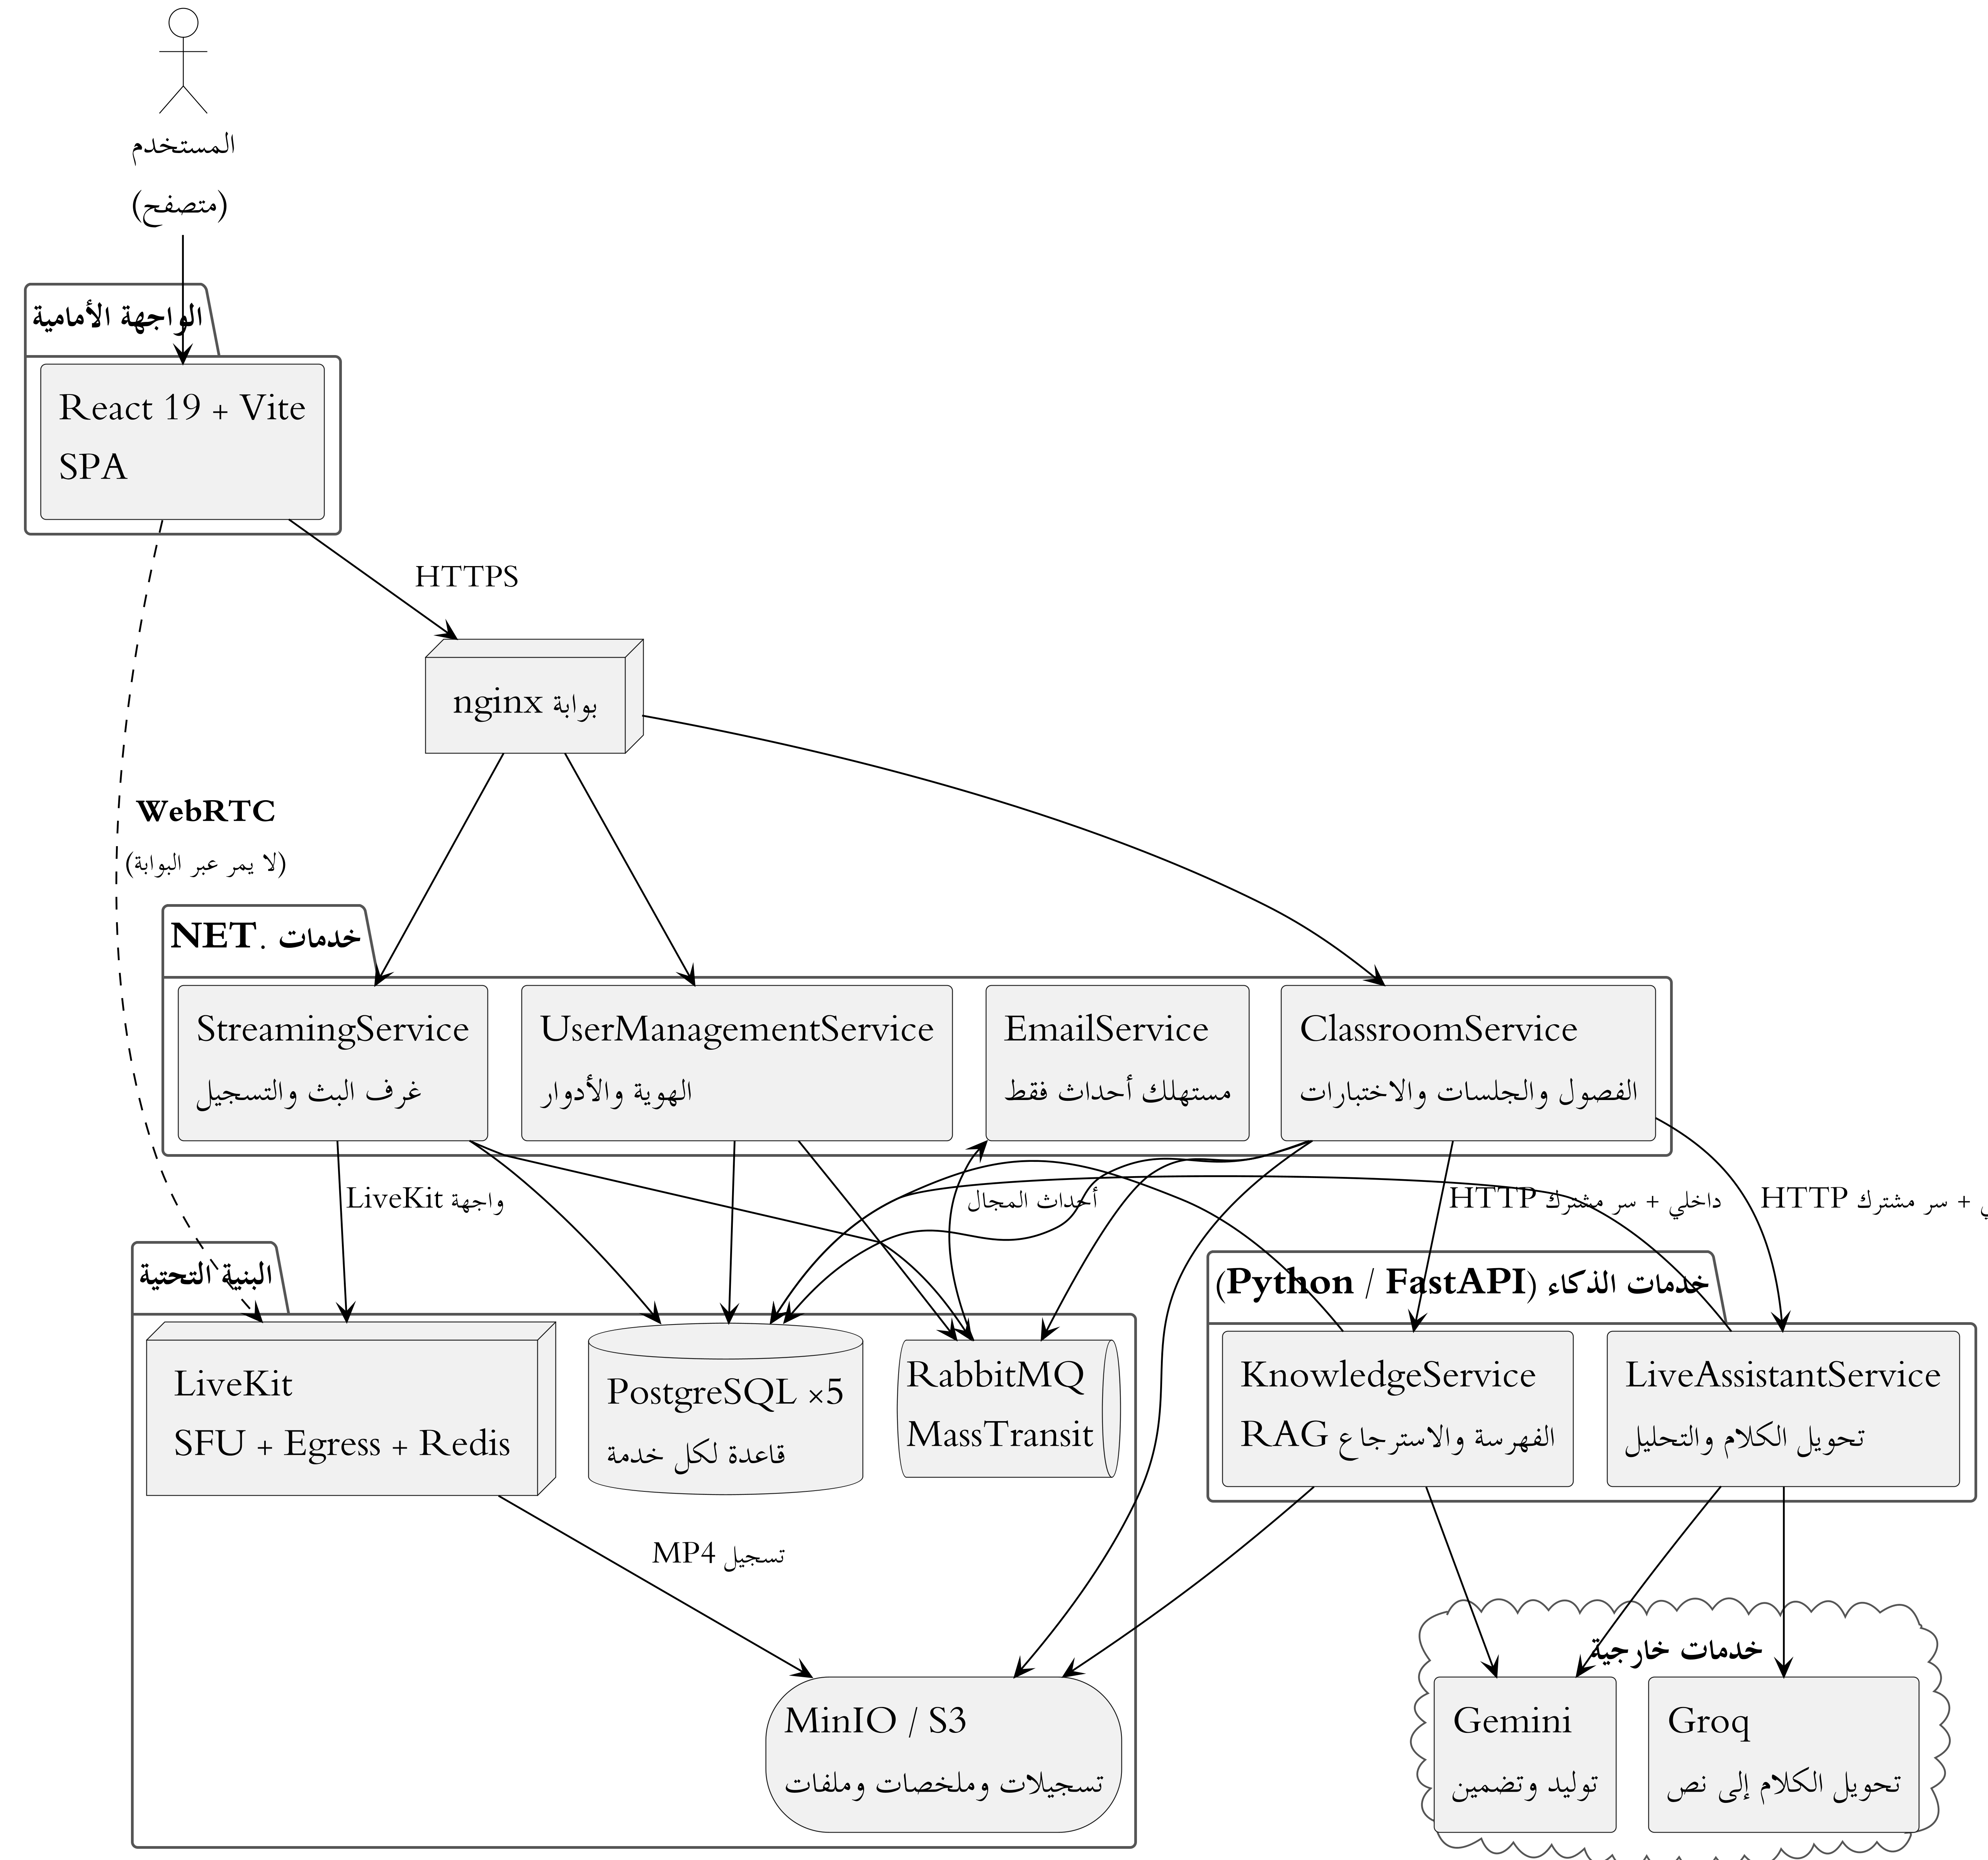
\includegraphics[width=\textwidth,height=0.8\textheight,keepaspectratio]{figures/arch-01-system-block.png}
  \caption{مخطط المكوّنات العام للنظام.}
  \label{fig:arch-01}
\end{figure}


\subsection{نمطا الاتصال بين الخدمات}

يقوم الاتصال بين الخدمات على نمطين أساسيين:

\begin{enumerate}
  \item \textbf{اتصال مباشر (متزامن) عبر \en{HTTP}}: يُستعمل حين تحتاج الخدمة إلى جواب قبل إكمال عملها. وتُعرَض هذه النقاط تحت المسار \en{/api/internal}، ولا تمرّ عبر البوّابة، ويحرسها سرٌّ مشترك يُرسَل في الترويسة \en{X-Internal-Secret}.
  \item \textbf{اتصال غير مباشر (غير متزامن) عبر ناقل الرسائل}: يُستعمل حين لا تحتاج الخدمة المرسِلة إلى جواب. ويُنفَّذ هذا النمط بالناقل \en{RabbitMQ} بوساطة \en{MassTransit}.
\end{enumerate}


\section{أنماط التصميم المعتمدة}
\label{sec:design-patterns}
% Content for Chapter 5, Section 5.2 — Design Patterns
تُعد أنماط التصميم (\en{Design Patterns}) بمثابة حلول معيارية لمشكلات هندسية متكررة في بناء الأنظمة البرمجية، حيث توفر لغة مشتركة للمطورين وتضمن استدامة الرماز المصدري. في مشروع \en{IntelliLect}، لم يكن الغرض من اعتماد هذه الأنماط مجرد الالتزام بالمعايير، بل كان الهدف الجوهري هو عزل الأجزاء المتغيرة عن الثابتة، وضمان قابلية النظام للاختبار (\en{Testability})، وتسهيل استبدال التقنيات الخارجية دون المساس بصلب منطق العمل.

يستعرض هذا القسم الأنماط الأساسية التي شكلت البنية التحتية للنظام، مع تبيان المبرر التقني لكل منها وموضع تطبيقه.

\subsection{قاعدة بيانات لكل خدمة (\en{Database per Service})}

يقضي هذا النمط بأن تمتلك كل خدمة مصغرة قاعدة بيانات خاصة بها حصرياً، بحيث يمتنع على أي خدمة أخرى الوصول إلى جداولها مباشرة. يعرض الشكل~\ref{fig:pattern-01} هذا المفهوم مطبّقاً على خدمتين من خدمات النظام.

\begin{figure}[htbp]
  \centering
  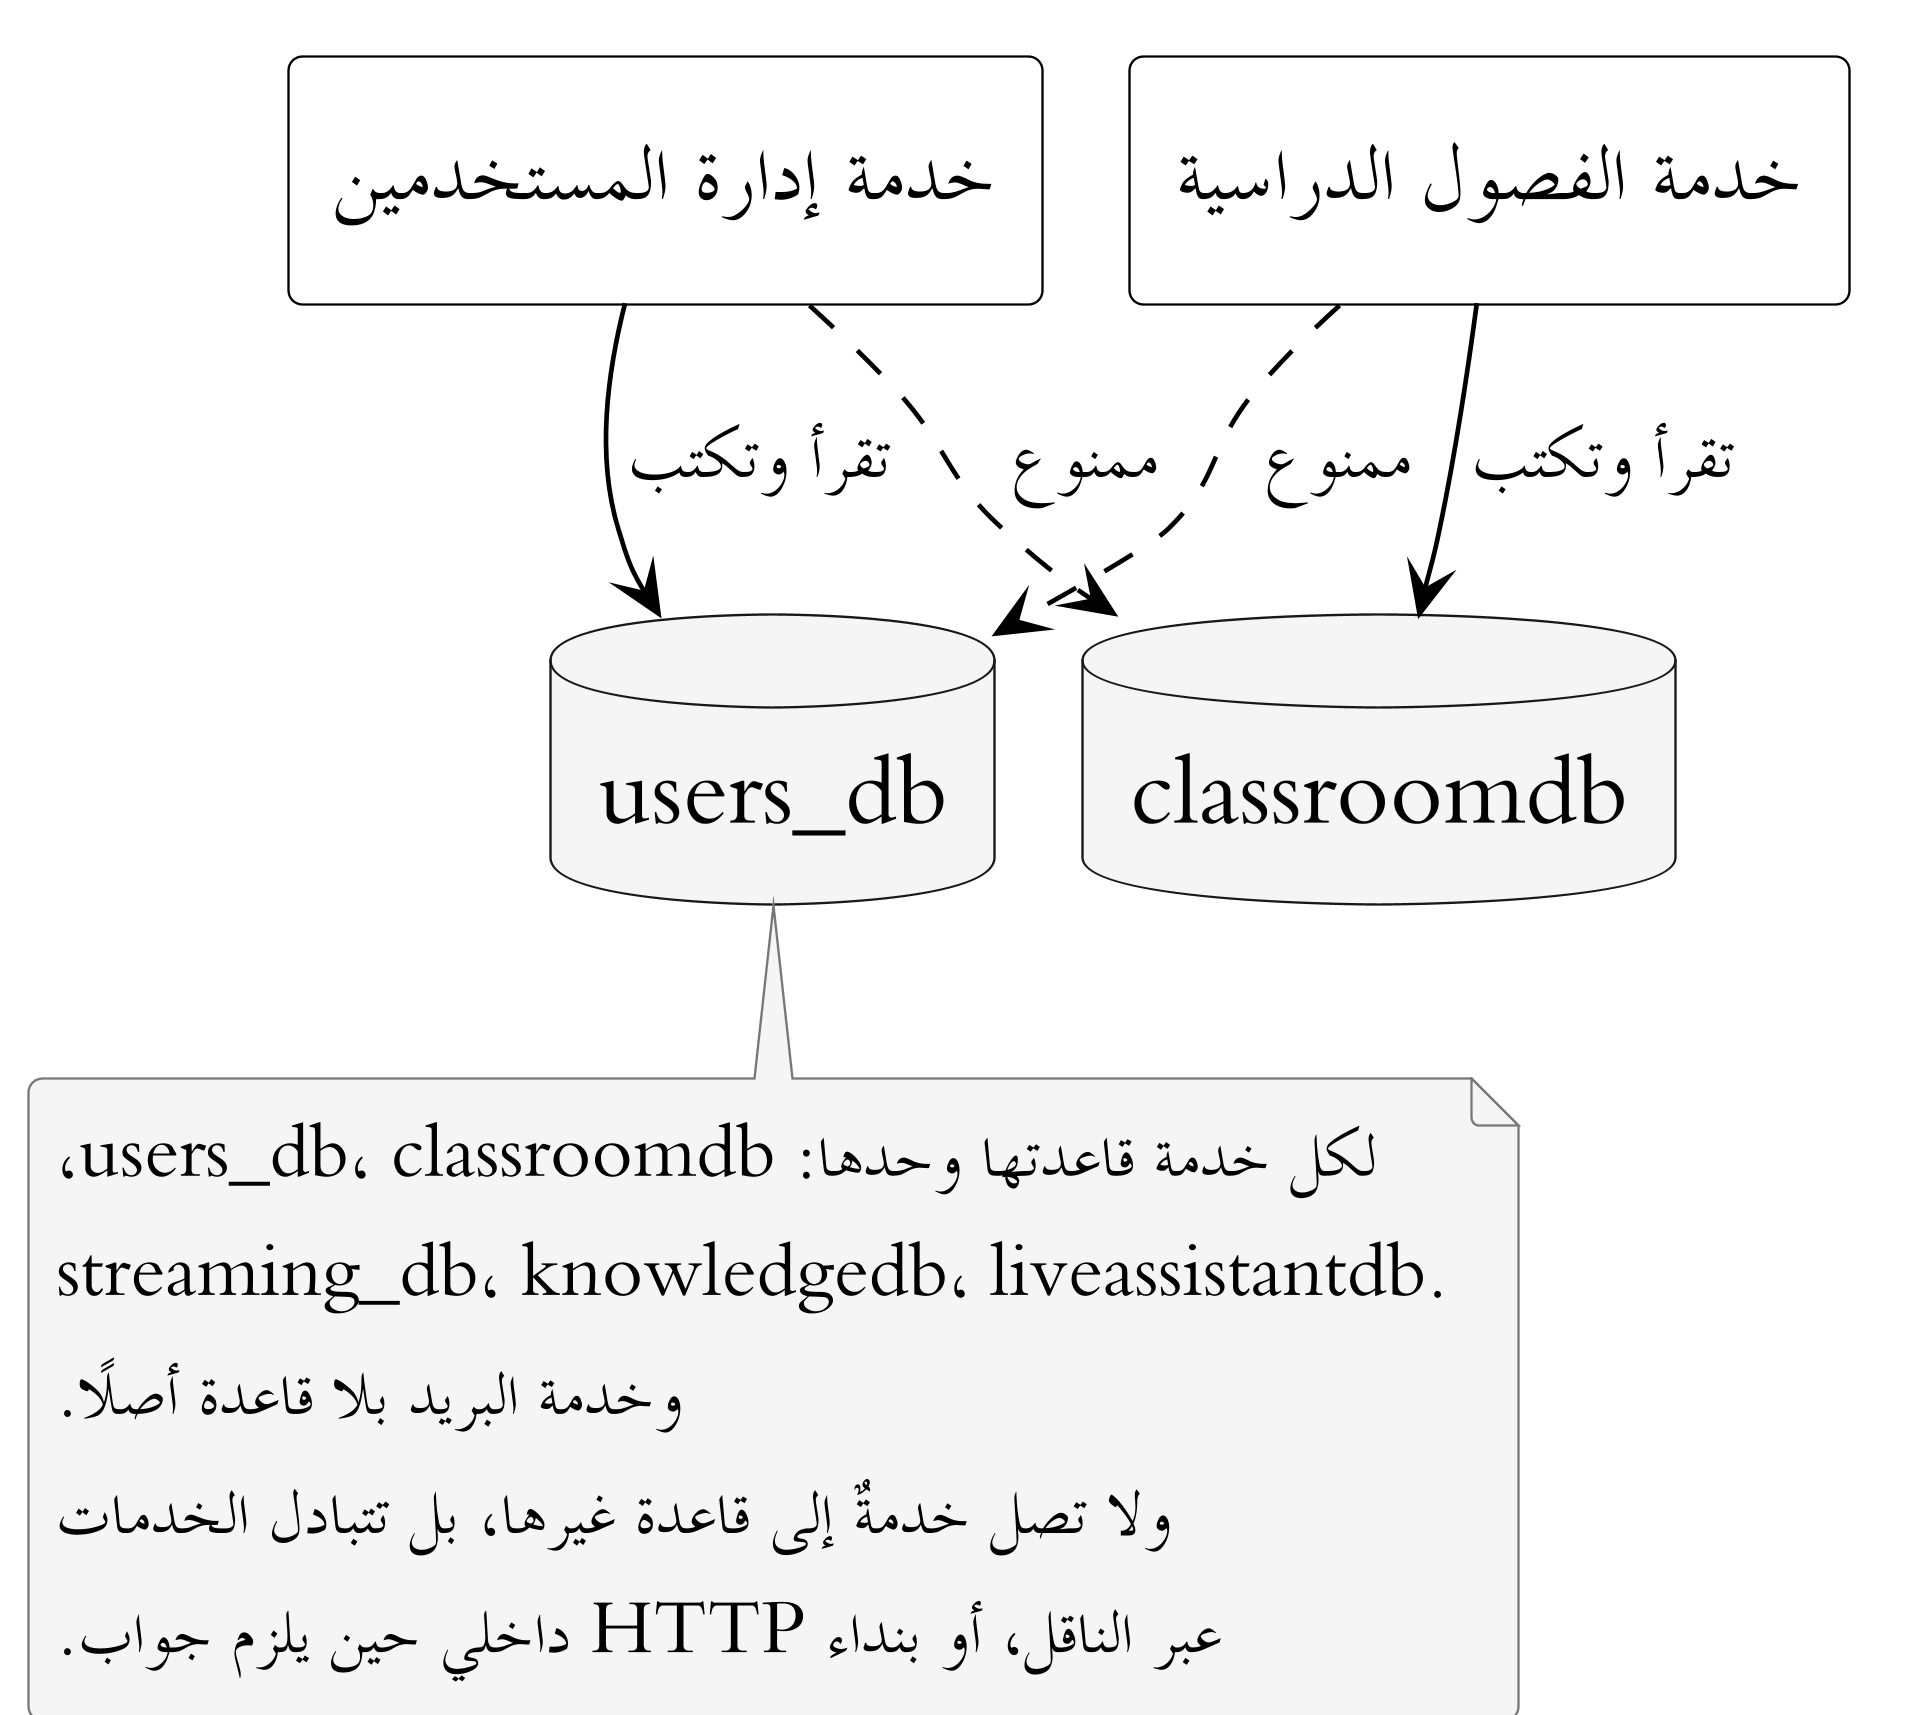
\includegraphics[width=\textwidth,height=0.8\textheight,keepaspectratio]{figures/pattern-01-database-per-service.png}
  \caption{نمط قاعدة بيانات لكل خدمة: تملك كل خدمة قاعدتها، والوصول المتقاطع ممنوع.}
  \label{fig:pattern-01}
\end{figure}

تكمن الغاية من هذا النمط في كسر الارتباط (\en{Coupling}) الذي قد ينشأ نتيجة مشاركة المخططات (\en{Schemas})؛ فحين تشترك خدمتان في قاعدة بيانات واحدة، يصبح أي تعديل في هيكلية الجداول بمثابة تغيير في "عقد ضمني" قد يؤدي إلى تعطل خدمات أخرى دون سابق إنذار. 

بناءً على هذا الأساس، تم تقسيم النظام إلى خمس قواعد بيانات منفصلة: \code{users\_db}، \code{classroomdb}، \code{streaming\_db}، \code{knowledgedb}، و\code{liveassistantdb}. وبالرغم من أن هذا الفصل استلزم استبدال الاستعلامات المباشرة (\en{Joins}) بنداءات بينية بين الخدمات، إلا أنه منحنا مرونة كاملة في تعديل وتوسيع كل خدمة بشكل مستقل.

\subsection{المنافذ والمحوِّلات (\en{Ports and Adapters})}

يهدف هذا النمط (المعروف أيضاً بالمعمارية السداسية) إلى فصل منطق التطبيق عن التفاصيل التقنية للوكلاء الخارجيين. يتم تعريف واجهات مجردة في طبقة التطبيق تسمى "المنافذ"، تصف الاحتياجات الوظيفية، بينما تتولى طبقة البنية التحتية توفير "المحوِّلات" التي تحقق هذه الواجهات. يوضح الشكل~\ref{fig:pattern-02} تطبيق هذا النمط في خدمة المعرفة.

\begin{figure}[htbp]
  \centering
  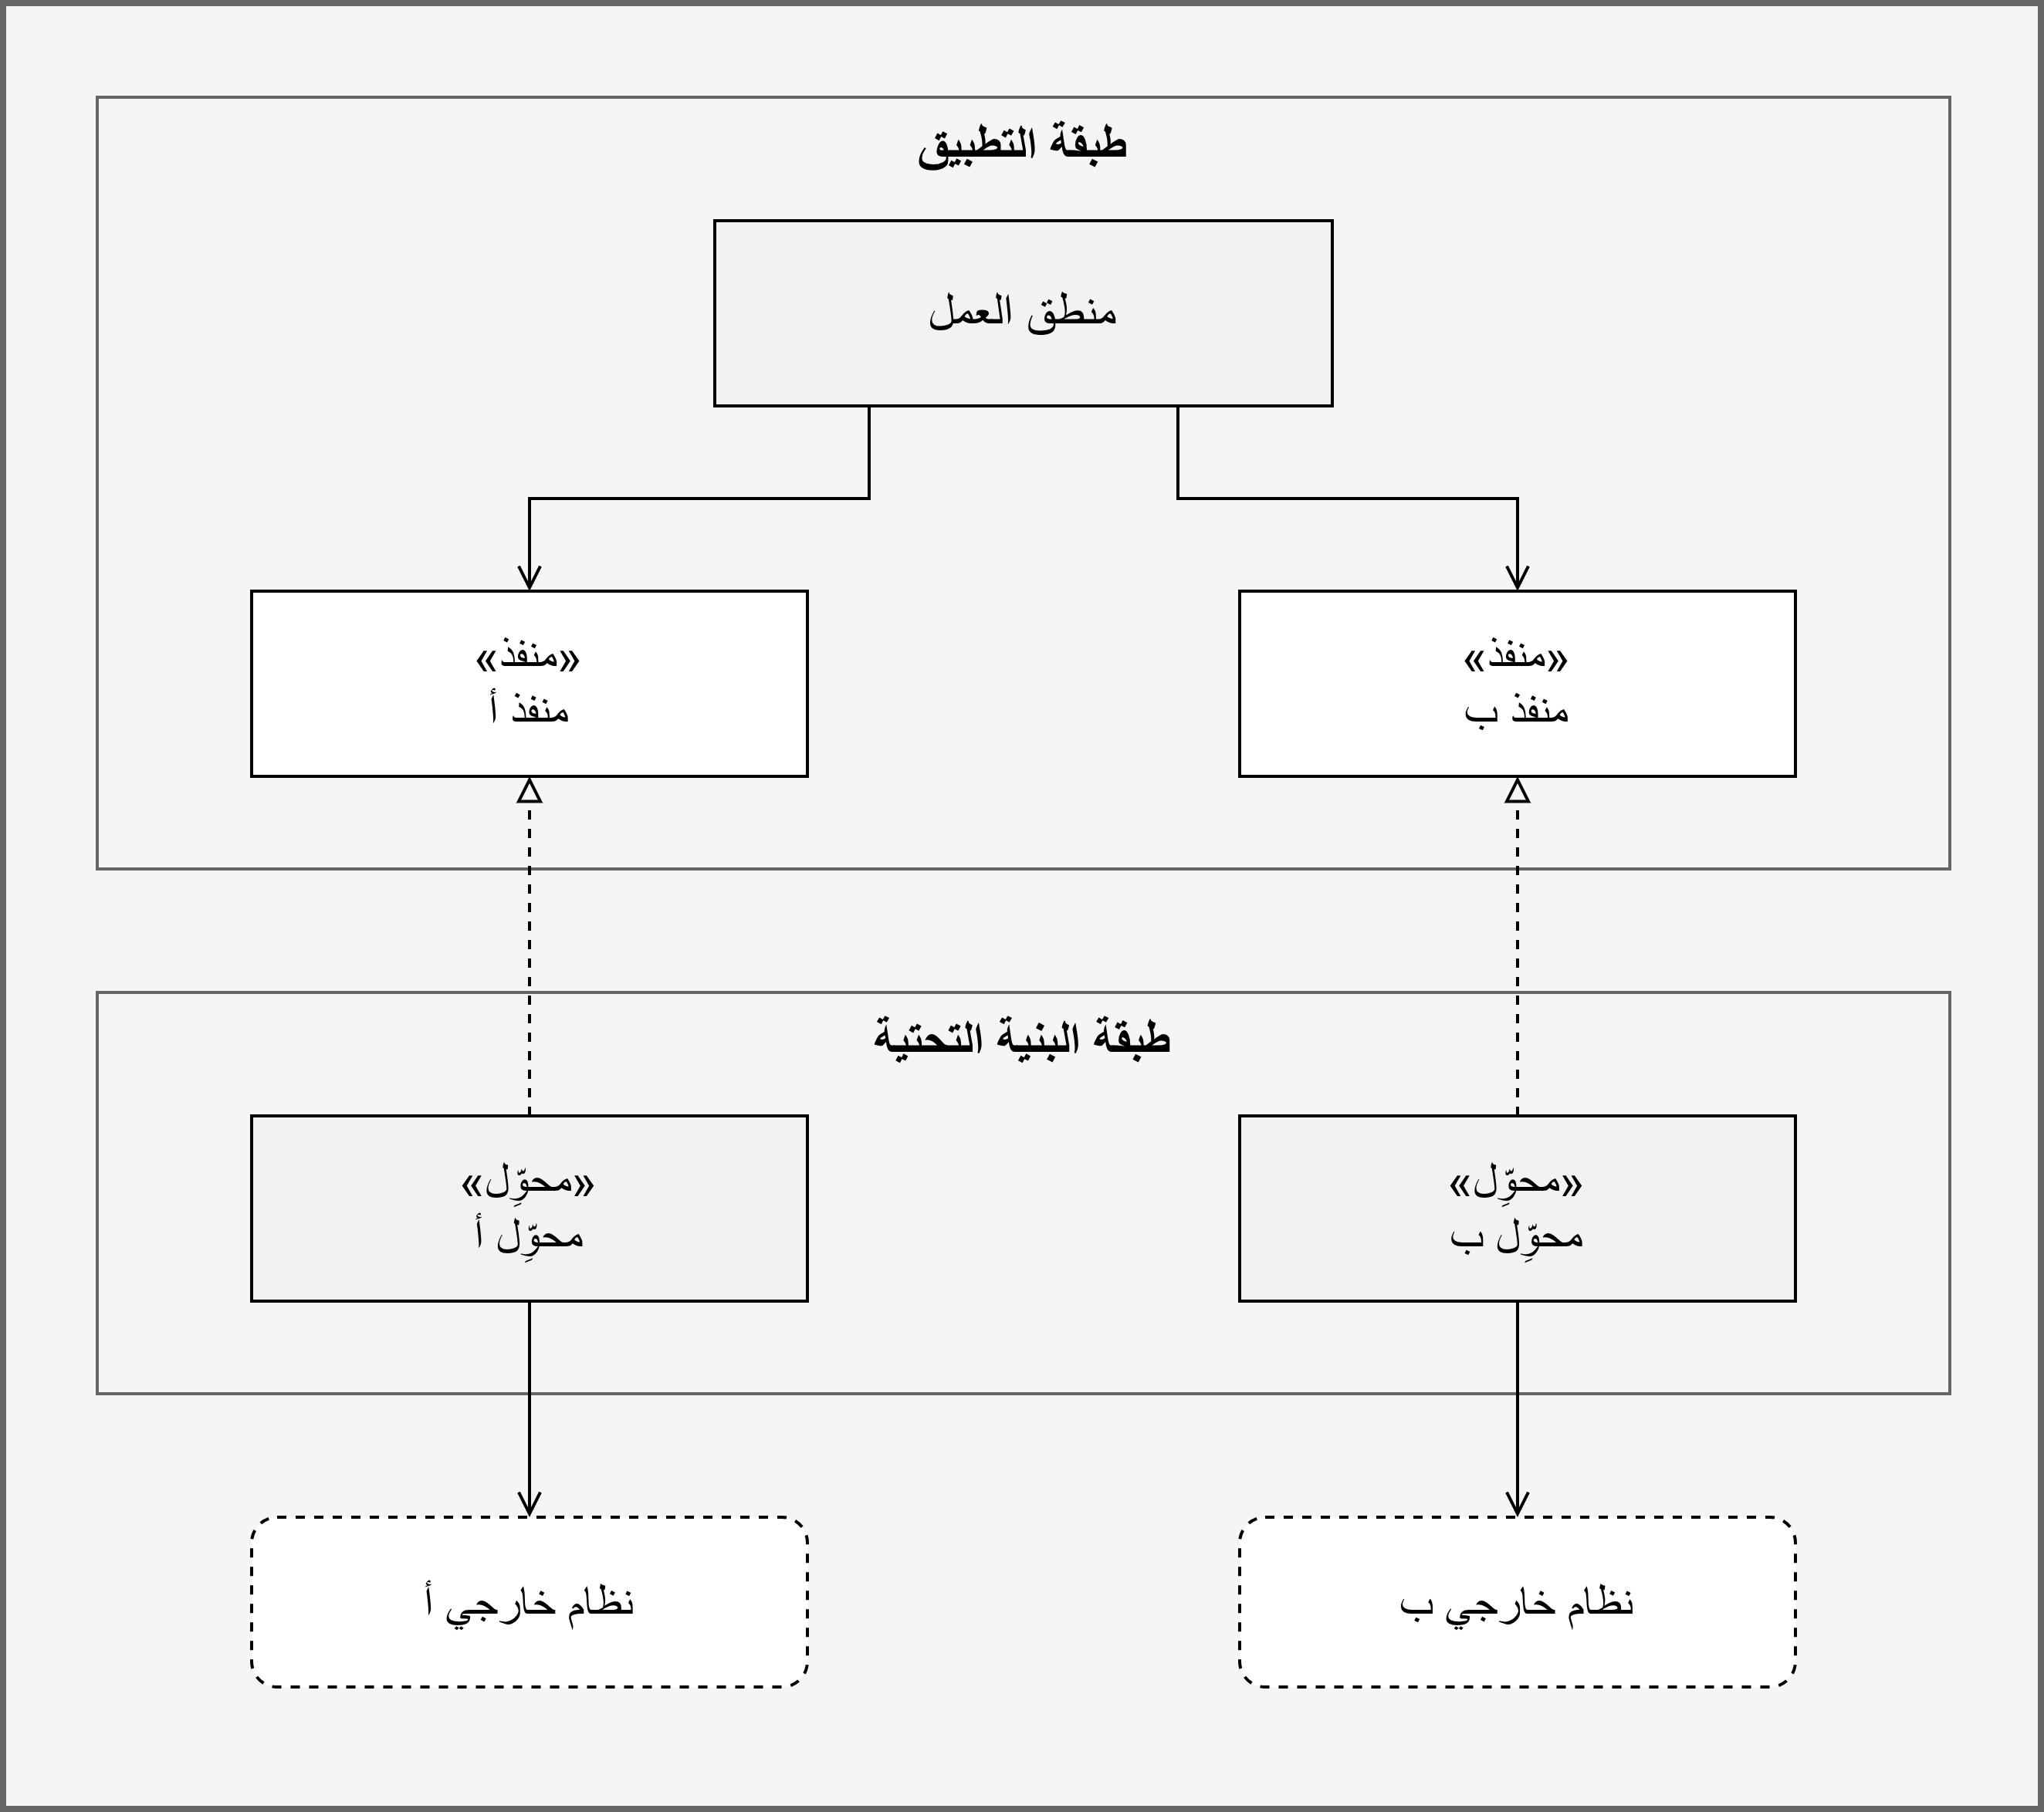
\includegraphics[width=\textwidth,height=0.8\textheight,keepaspectratio]{figures/pattern-02-ports-adapters.png}
  \caption{نمط المنافذ والمحوِّلات: المنفذ يُعرَّف في طبقة التطبيق، والمحوِّل يحقّقه في طبقة البنية التحتية.}
  \label{fig:pattern-02}
\end{figure}

يعالج هذا النمط مشكلة التبعية للتقنيات الخارجية؛ فبدلاً من أن يرتبط منطق العمل بمزود خدمة معين، تصبح الطبقة الداخلية هي التي تملي ما تحتاجه، والخارجية هي التي تلبي ذلك. وقد تم تعريف 14 منفذاً في خدمة المعرفة و8 في خدمة المساعد الحي، مما أتاح لنا اختبار المنطق البرمجي بمعزل عن قواعد البيانات أو خوادم الويب.

\subsection{الاستراتيجية (\en{Strategy})}

يعتمد هذا النمط على تعريف عائلة من الخوارزميات وجعلها قابلة للاستبدال عبر واجهة موحدة، بحيث يمكن للمستدعي استخدام أي منها دون معرفة تفاصيل تنفيذها. يوضح الشكل~\ref{fig:pattern-03} استراتيجيات تحويل الكلام إلى نص (\en{STT}).

\begin{figure}[htbp]
  \centering
  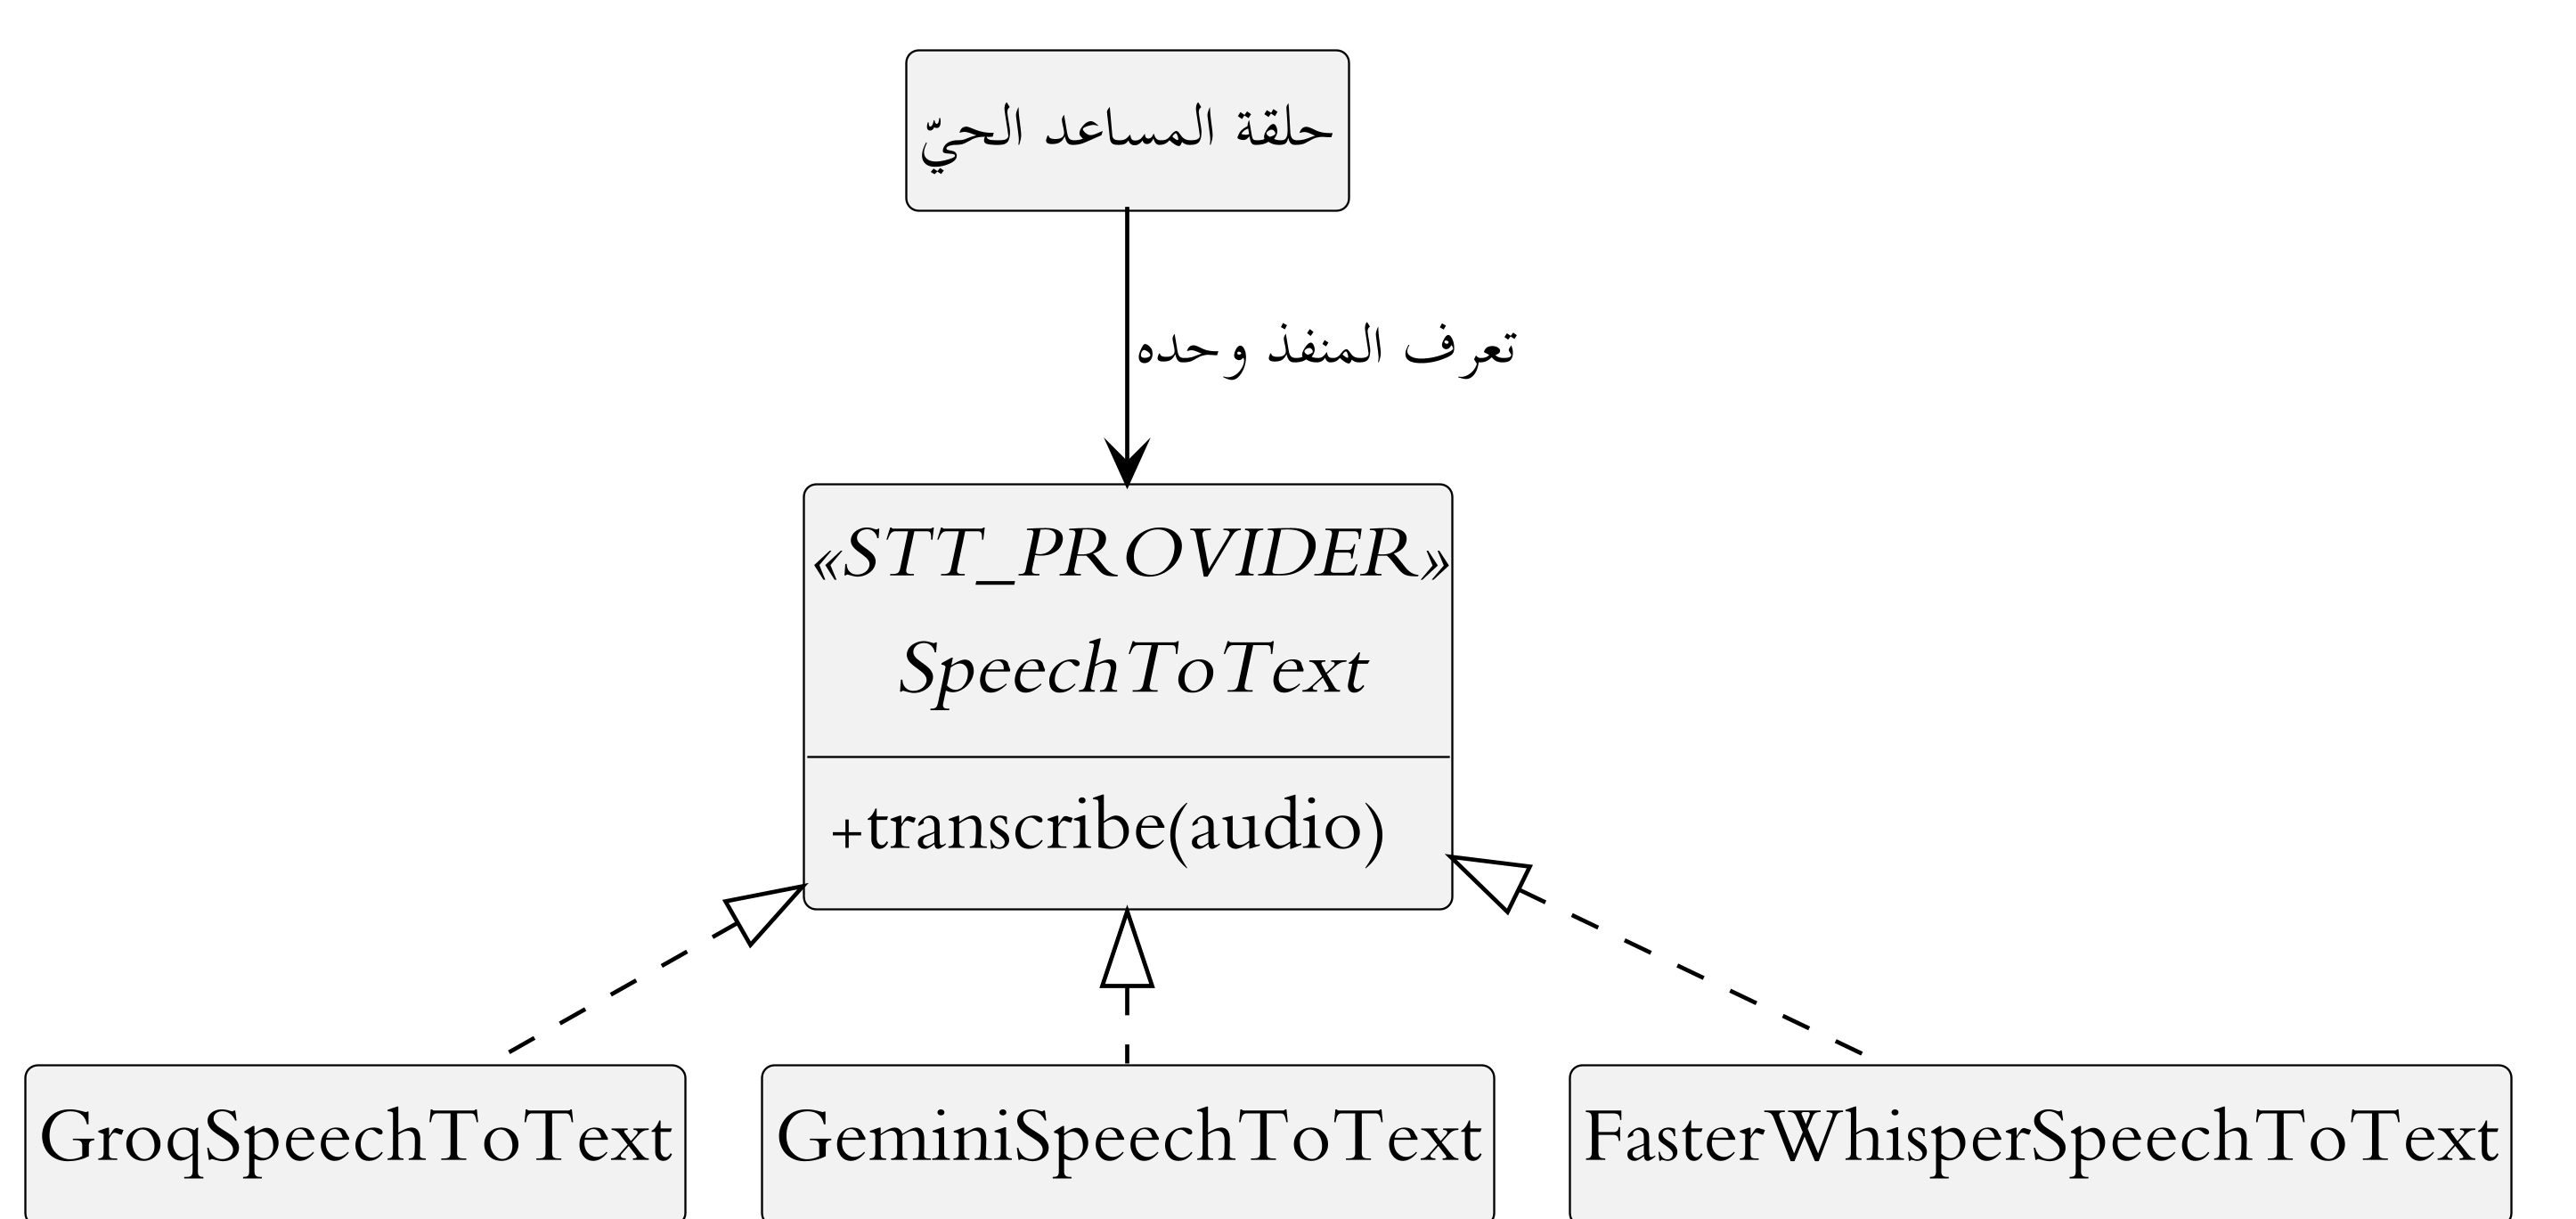
\includegraphics[width=\textwidth,height=0.8\textheight,keepaspectratio]{figures/pattern-03-strategy.png}
  \caption{نمط الاستراتيجية: منفذٌ واحد وثلاثة تحقيقات متكافئة، والمستدعي لا يعرف إلّا المنفذ.}
  \label{fig:pattern-03}
\end{figure}

استُخدم هذا النمط في المواضع التي تتطلب مفاضلة بين بدائل تقنية؛ مثل اختيار نموذج التضمين (\en{Embedding}) أو محرك تحويل الكلام. بفضل هذا النمط، أمكننا الانتقال من النماذج المحلية إلى المستضافة (مثل \en{Gemini}) أو العكس عبر تغيير بسيط في الإعدادات، دون تعديل شيفرة منطق العمل الأساسية.

\subsection{المصنع (\en{Factory})}

يعمل نمط المصنع كمتمم لنمط الاستراتيجية، حيث يتولى مسؤولية اختيار الاستراتيجية المناسبة وإنشائها بناءً على الحالة الراهنة أو الإعدادات، حاجباً بذلك منطق الاختيار عن المستهلك. يعرض الشكل~\ref{fig:pattern-04} مصنع المقسِّمات (\en{Chunkers}) في خدمة المعرفة.

\begin{figure}[htbp]
  \centering
  % Narrower than the rest on purpose: five boxes in four ranks come out taller
  % than wide, and at full width the figure fills the page and floats alone.
  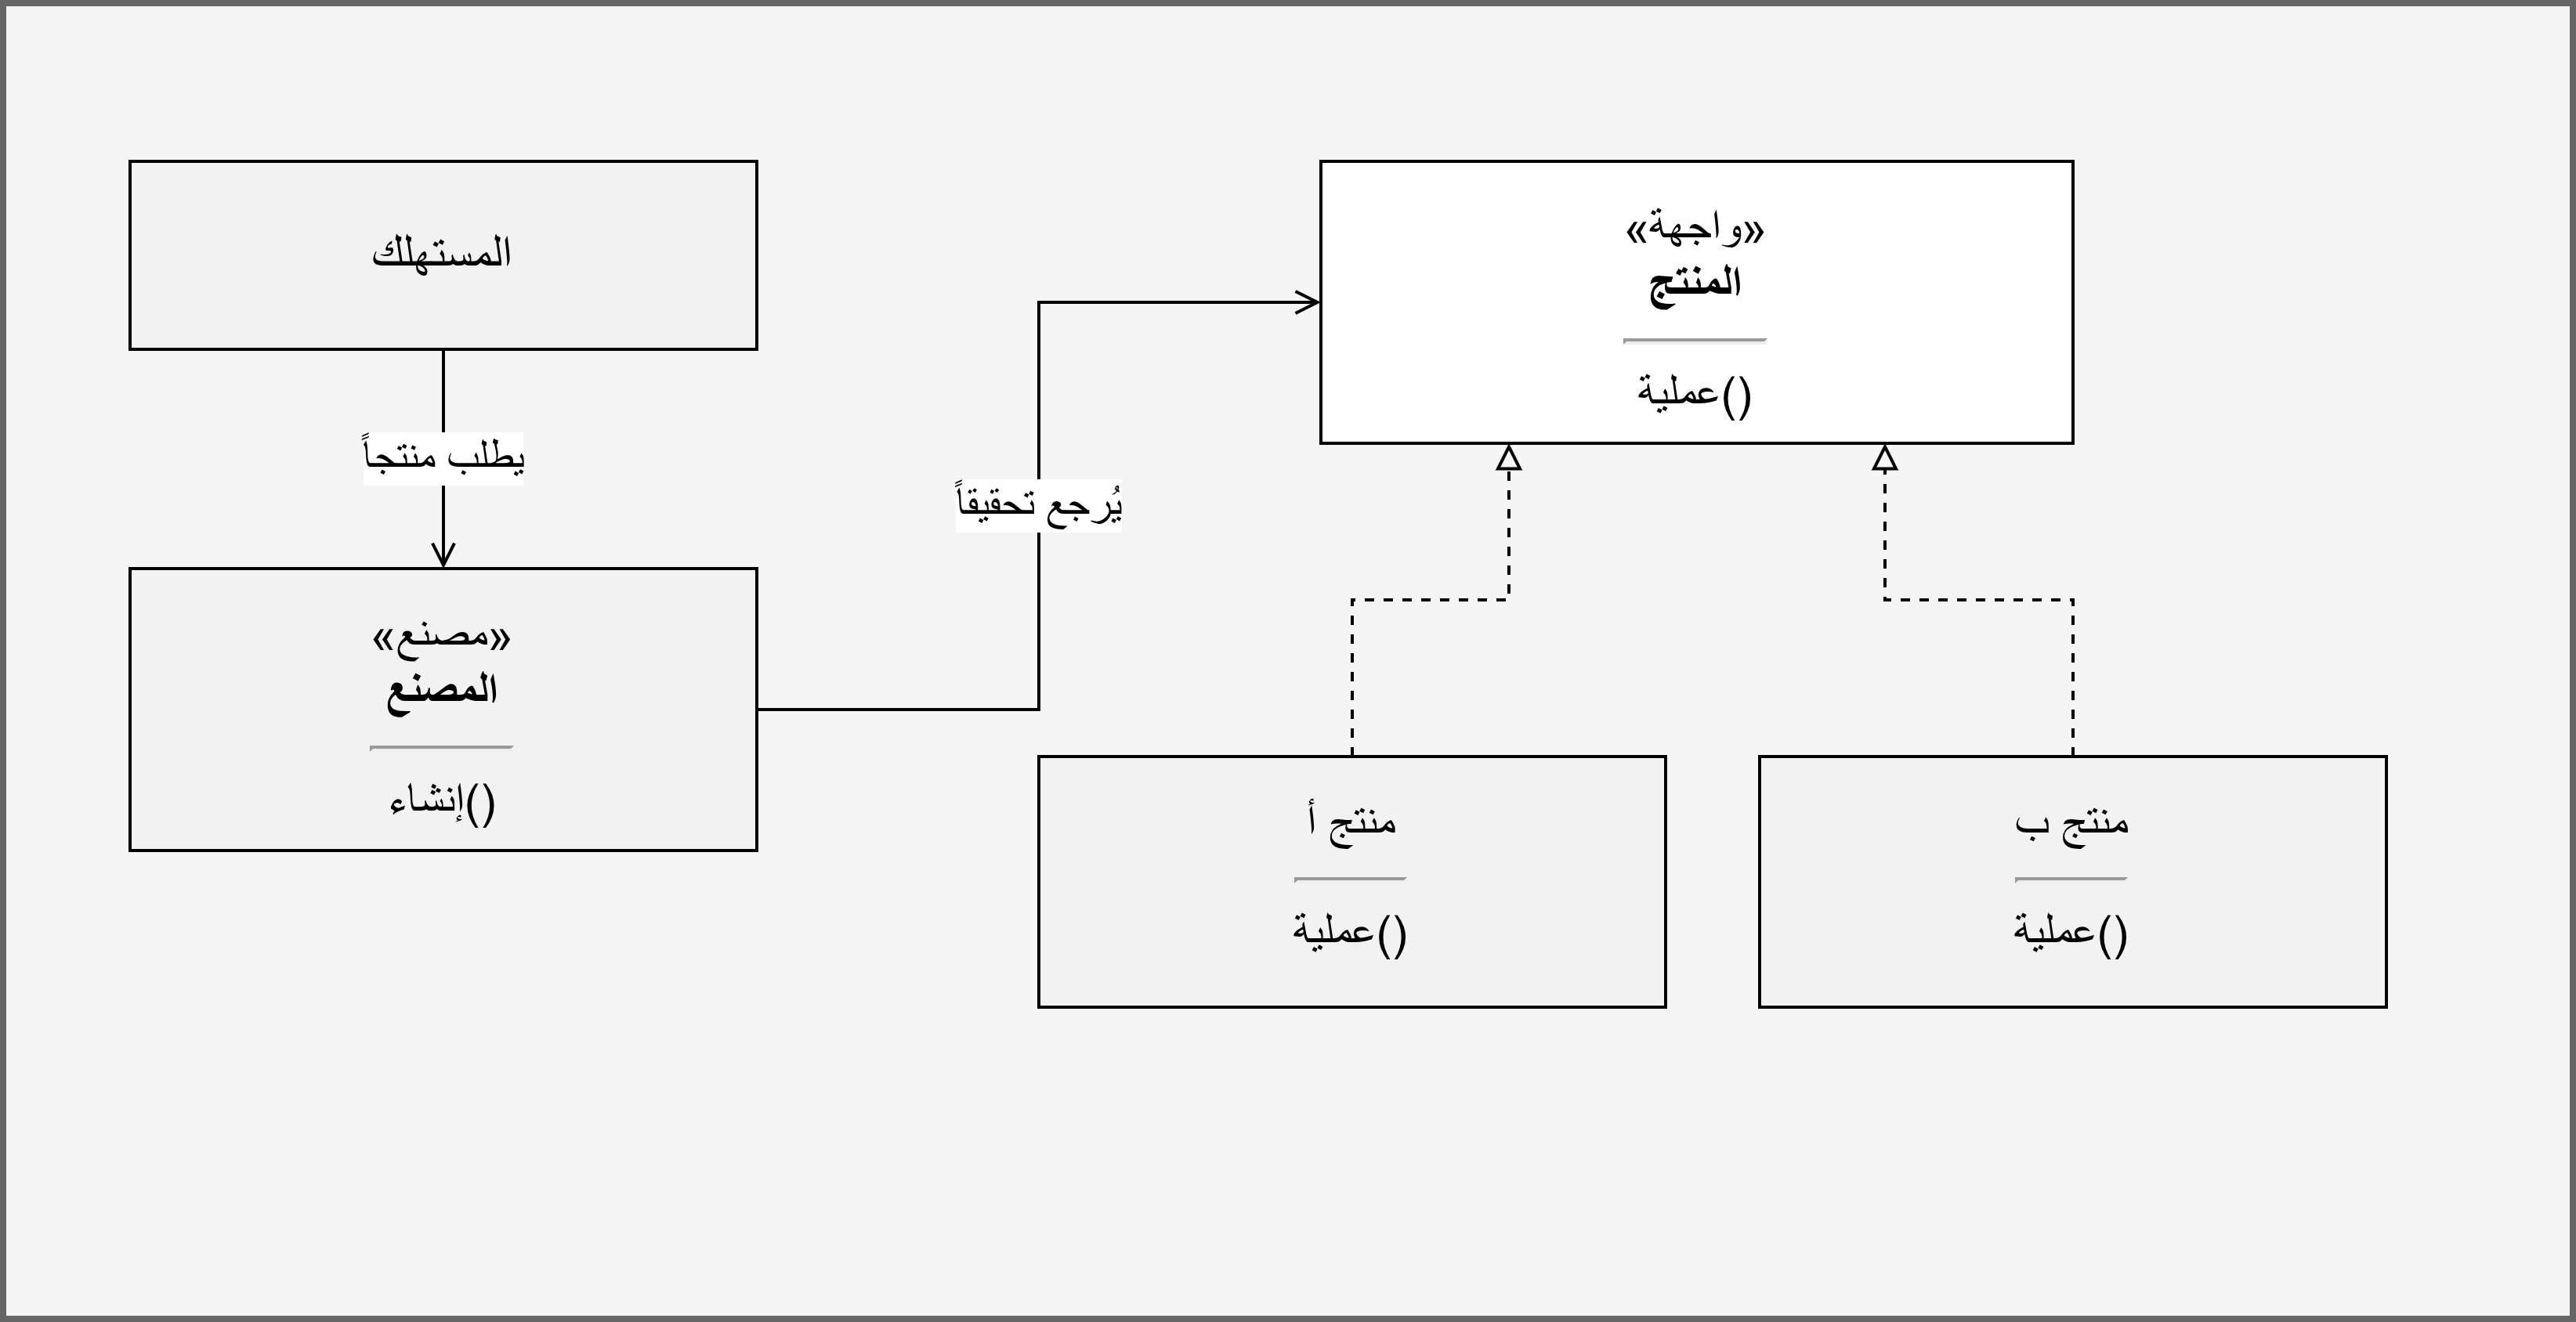
\includegraphics[width=0.6\textwidth,height=0.8\textheight,keepaspectratio]{figures/pattern-04-factory.png}
  \caption{نمط المصنع: المستدعي يطلب مقسِّمًا فيتلقّى تحقيقًا للمنفذ، دون أن يعرف أيَّها.}
  \label{fig:pattern-04}
\end{figure}

في نظامنا، نجد تطبيقات عديدة لهذا النمط، مثل \code{create\_chunker} الذي يقرأ إعدادات التقطيع ويُرجع الاستراتيجية الموافقة، و\code{ExtractorRouter} الذي يحدد المستخرج المناسب حسب نوع الملف المرفوع، مما يضمن بقاء منطق الاستدعاء بسيطاً ومركزاً على المهمة الوظيفية.

\subsection{المستودع (\en{Repository})}

يحجب نمط المستودع آليات الوصول إلى البيانات (مثل استعلامات \en{SQL} أو \en{ORM}) خلف واجهة تتحدث بلغة "المجال التعليمي". يعرض الشكل~\ref{fig:pattern-05} تحقيق هذا النمط في خدمات \en{.NET} عبر قاعدة بيانات عامة.

\begin{figure}[htbp]
  \centering
  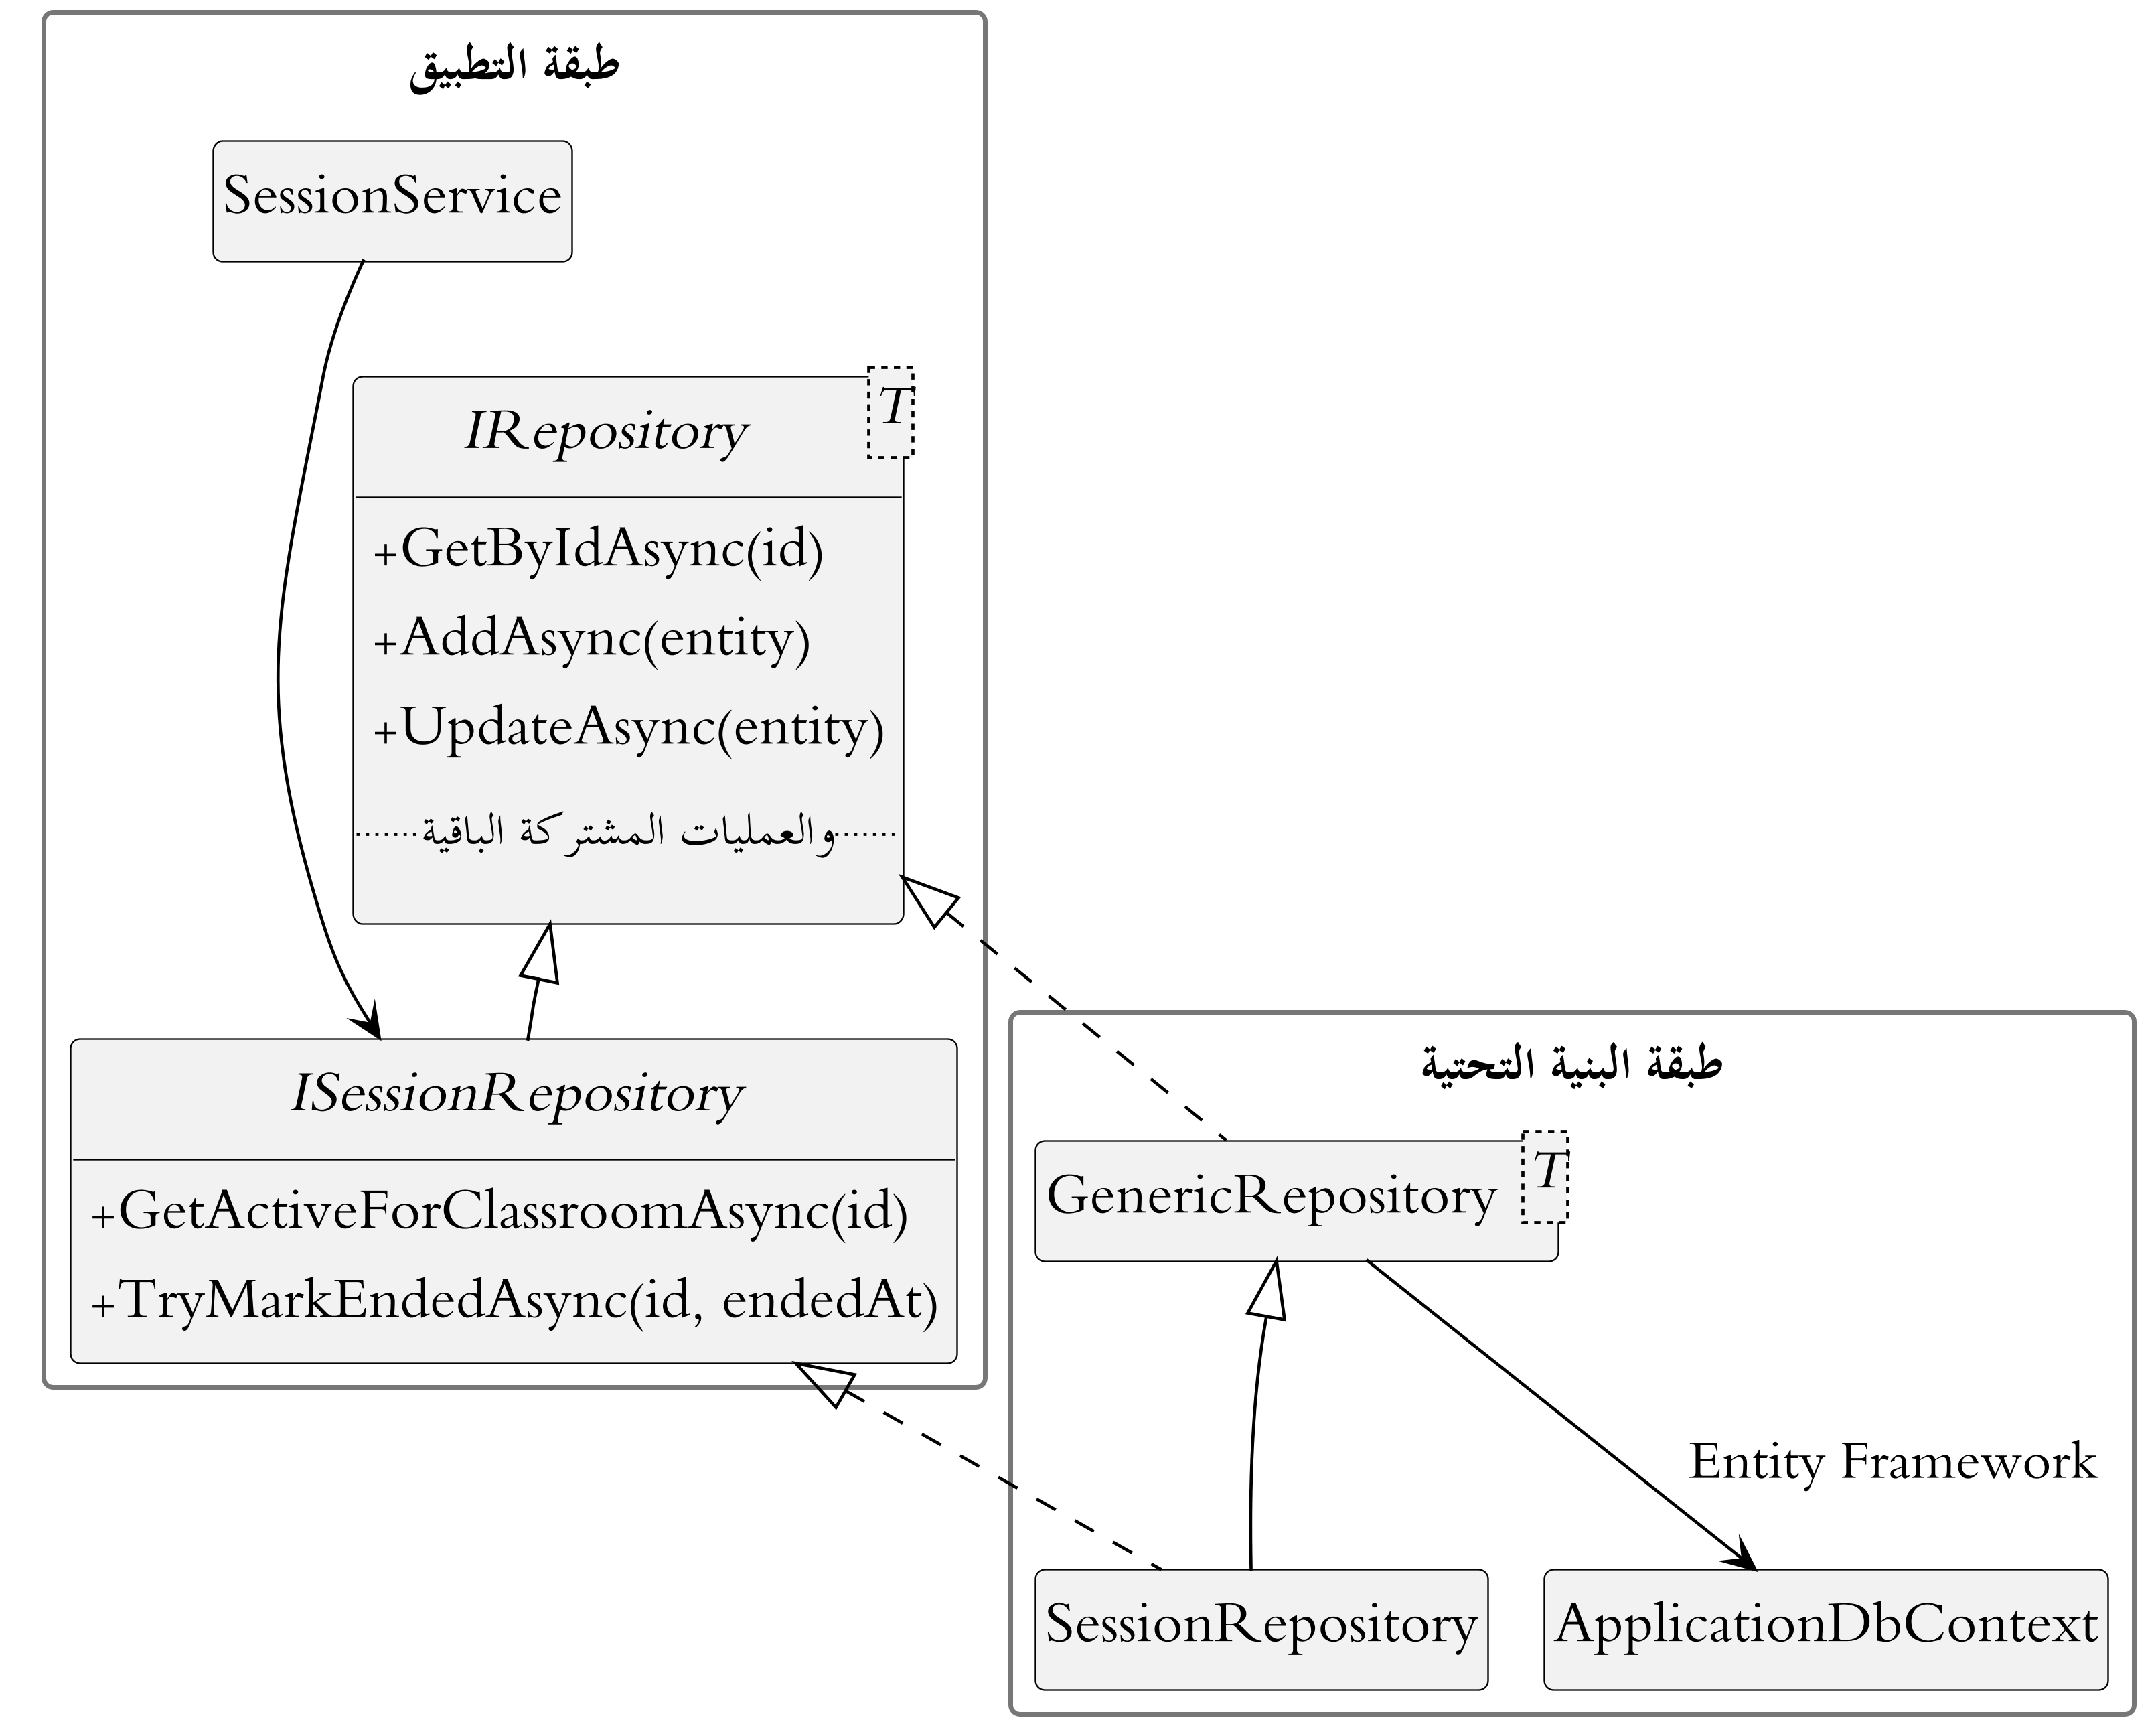
\includegraphics[width=\textwidth,height=0.8\textheight,keepaspectratio]{figures/pattern-05-repository.png}
  \caption{نمط المستودع بقاعدة عامّة: تُعرَّف الواجهة في طبقة التطبيق وتُحقَّق في طبقة البنية التحتية.}
  \label{fig:pattern-05}
\end{figure}

تكمن ميزة هذا النمط في عزل طبقة التطبيق عن مكتبات الوصول إلى البيانات مثل \en{Entity Framework}. وقد اعتمدنا مستودعاً عاماً \code{GenericRepository<T>} يحمل العمليات المتكررة، ورثته عشرة مستودعات متخصصة، مما مكننا من إجراء الاختبارات الوحدوية باستخدام مستودعات وهمية تعمل في الذاكرة دون الحاجة لقاعدة بيانات حقيقية.

\subsection{وحدة العمل (\en{Unit of Work})}

يضمن نمط وحدة العمل جمع عدة عمليات كتابة ضمن معاملة واحدة (\en{Transaction})، بحيث تنجح جميعها معاً أو تُلغى جميعاً، مما يحافظ على اتساق البيانات. يوضح الشكل~\ref{fig:pattern-06} مسار إنهاء الجلسة كمثال على هذا النمط.

\begin{figure}[htbp]
  \centering
  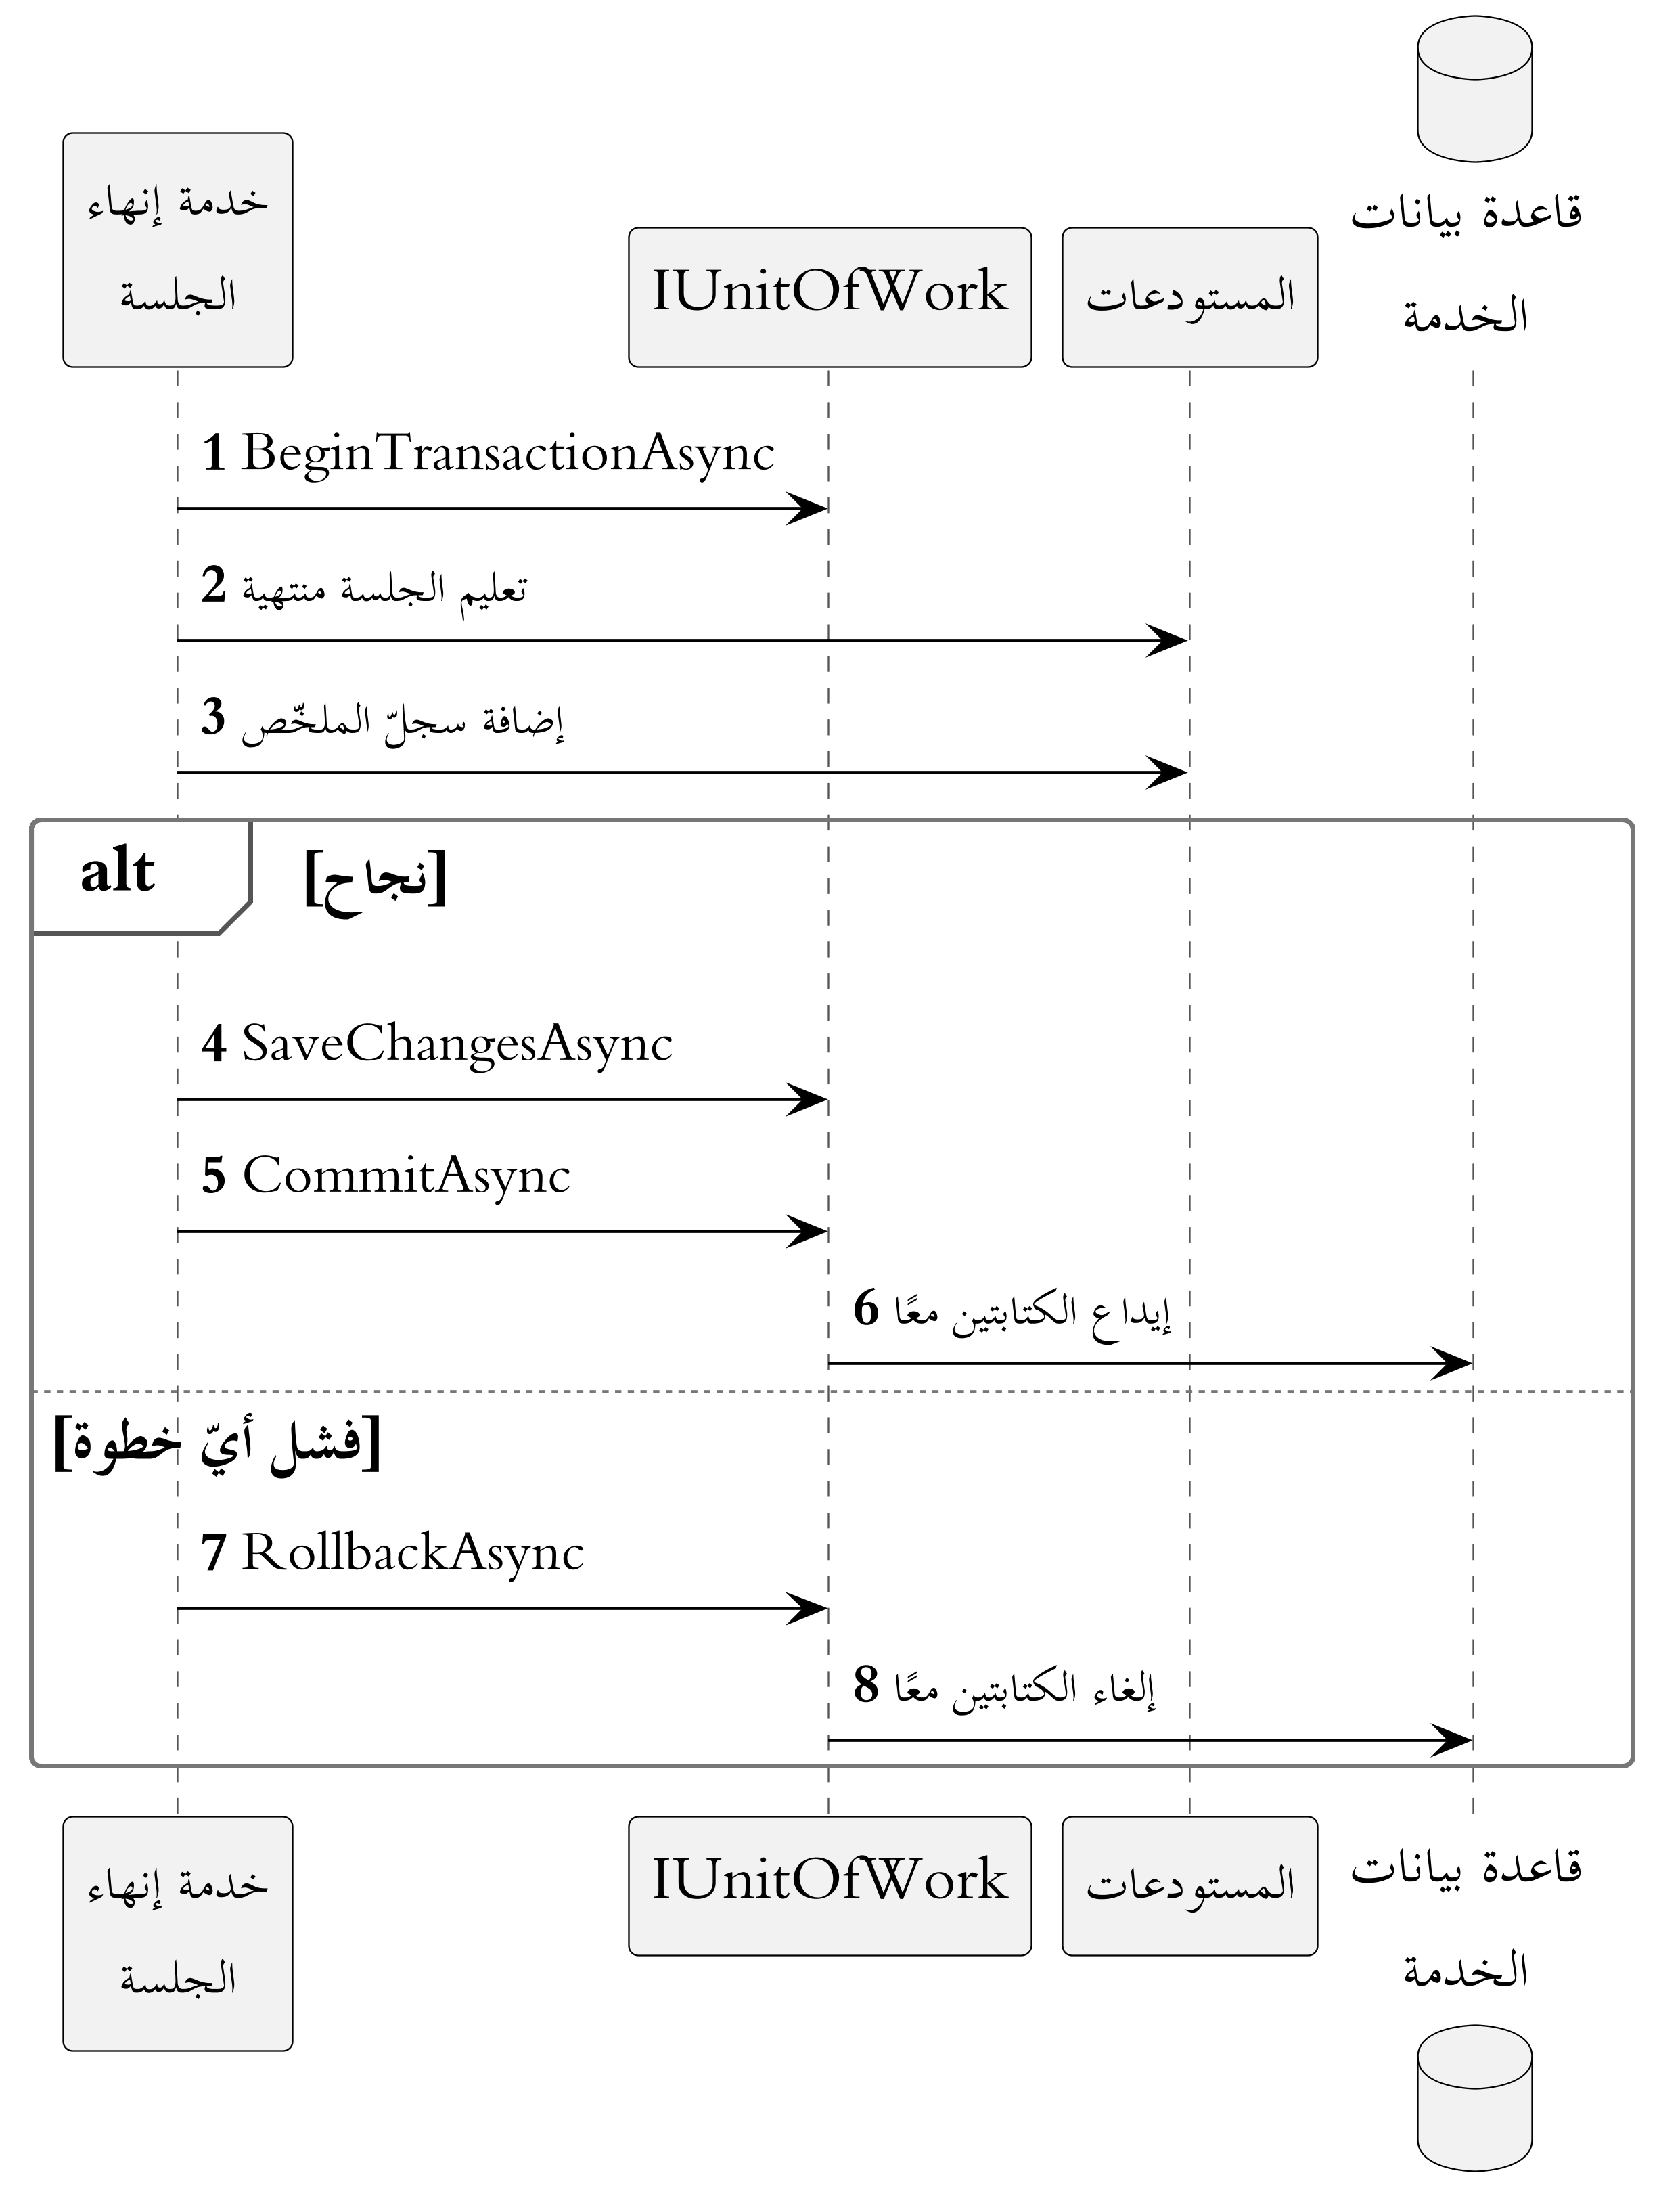
\includegraphics[width=\textwidth,height=0.8\textheight,keepaspectratio]{figures/pattern-06-unit-of-work.png}
  \caption{نمط وحدة العمل: كتابتان عبر مستودعين تحت معاملةٍ واحدة، تُودَعان معًا أو تُلغَيان معًا.}
  \label{fig:pattern-06}
\end{figure}

يعالج هذا النمط مخاطر "البيانات المتناقضة"؛ ففي عملية إنهاء الجلسة، يجب تحديث حالة الجلسة وإضافة سجل الملخص في آن واحد. لولا وحدة العمل، لكان من الممكن تحديث الجلسة وفشل إضافة سجل الملخص، مما يترك النظام في حالة غير متسقة. يوفر المنفذ \code{IUnitOfWork} العمليات اللازمة لإيداع (\en{Commit}) أو إلغاء (\en{Rollback}) المعاملة بشكل آمن.

\subsection{صندوق الصادر المعامل (\en{Transactional Outbox})}

يعد هذا النمط حلاً لمشكلة عدم إمكانية إجراء معاملة ذرية بين قاعدة البيانات وناقل الرسائل (\en{Message Bus}). يعرض الشكل~\ref{fig:pattern-07} آلية عمل هذا النمط لضمان تسليم الأحداث.

\begin{figure}[htbp]
  \centering
  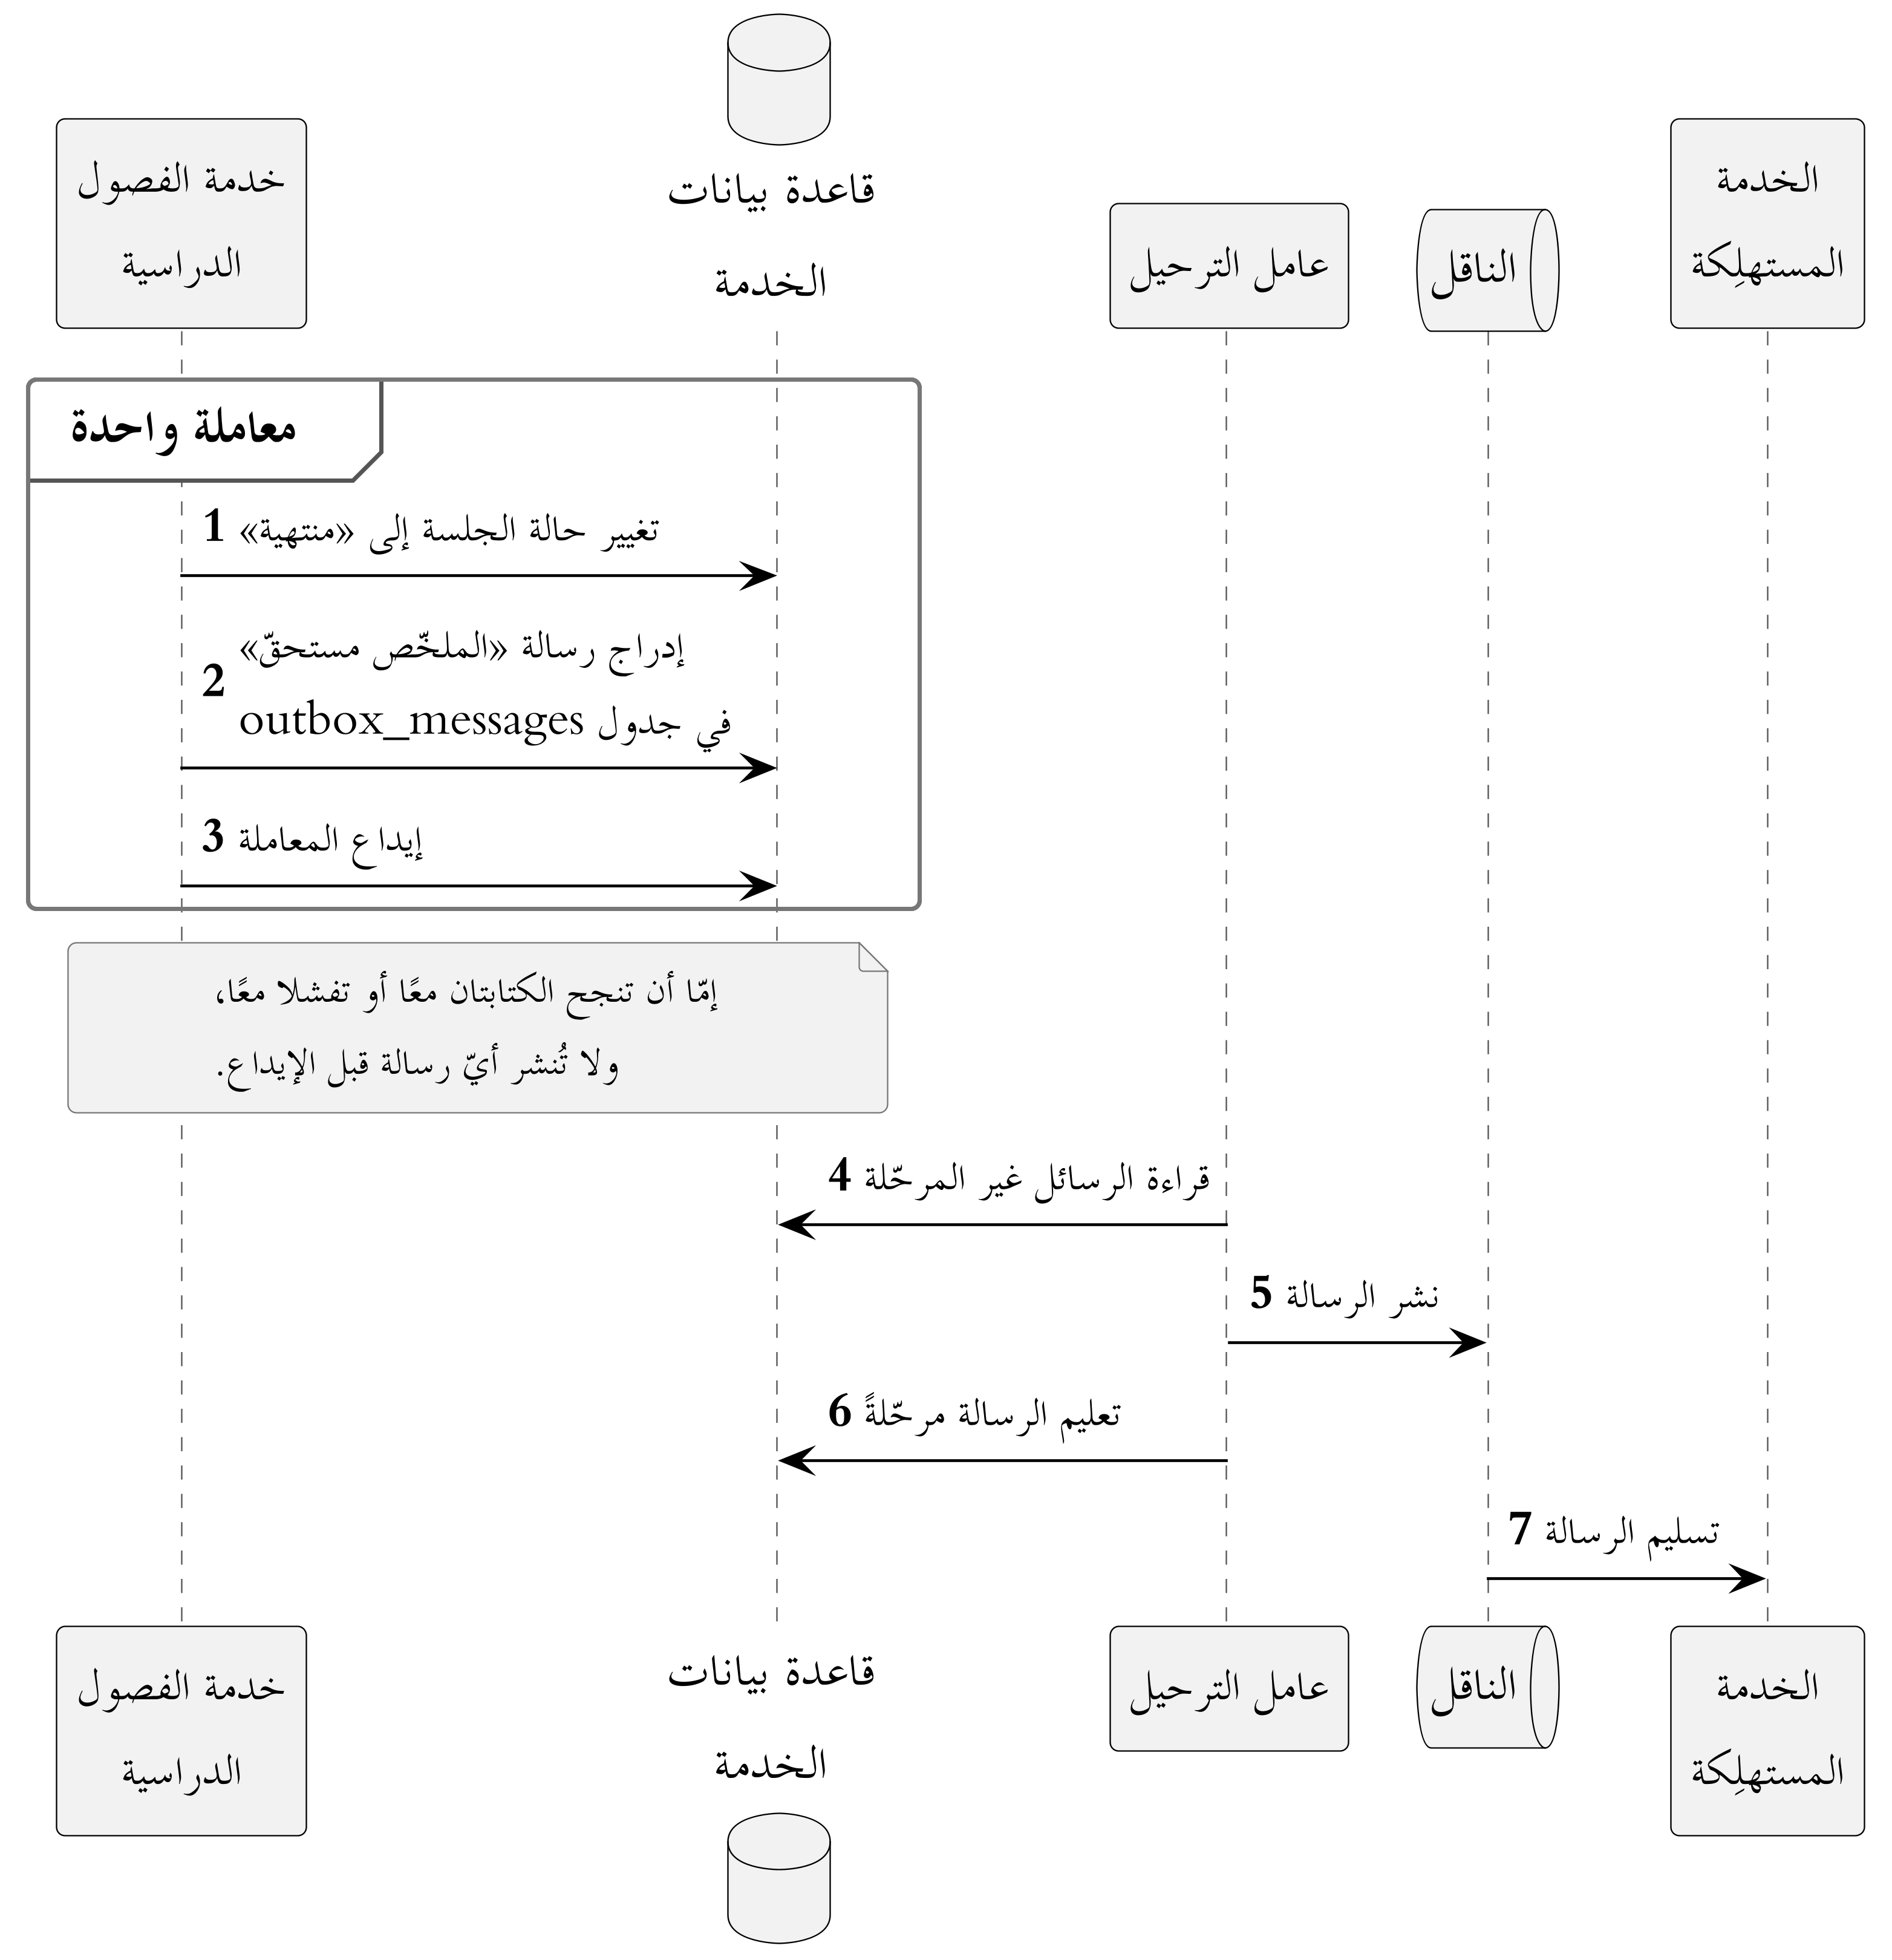
\includegraphics[width=\textwidth,height=0.8\textheight,keepaspectratio]{figures/pattern-07-transactional-outbox.png}
  \caption{نمط صندوق الصادر المعامل: تُكتَب الرسالة ضمن معاملة العمل، ثمّ يُرحّلها عامل مستقلّ.}
  \label{fig:pattern-07}
\end{figure}

عند إنهاء جلسة أو توليد ملخص، تُكتب الرسالة في جدول خاص (\code{outbox\_messages}) ضمن نفس معاملة قاعدة البيانات التي تُغير الحالة. لاحقاً، يتولى عامل ترحيل مستقل قراءة هذه الرسائل ونشرها على الناقل. يضمن هذا الإجراء وصول الإشعارات إلى الخدمات المستهلكة حتى في حال تعطل الناقل لحظياً، حيث تبقى الرسائل في الصادر حتى يتم التأكد من نشرها بنجاح.

\section{مكوّنات تطبيق الويب}
% Content for Chapter 5, Section 5.3 — pulled in by chapters/05-system-design.tex
بُني تطبيق الويب بمكتبة \en{React 19} فوق أداة البناء \en{Vite}، وقُسّم إلى شرائح وظيفية (\en{Feature Slices}) لا إلى طبقات تقنية. وتملك كل شريحة مجلّداتها الأربعة: \en{api} لنداءات الخدمات، و\en{hooks} لحالة الخادم، و\en{components} لعناصر الواجهة، و\en{types} لأنماط البيانات. ويعرض الشكل~\ref{fig:comp-07} هذه المكوّنات مع روابطها الخارجية.

\begin{figure}[htbp]
  \centering
  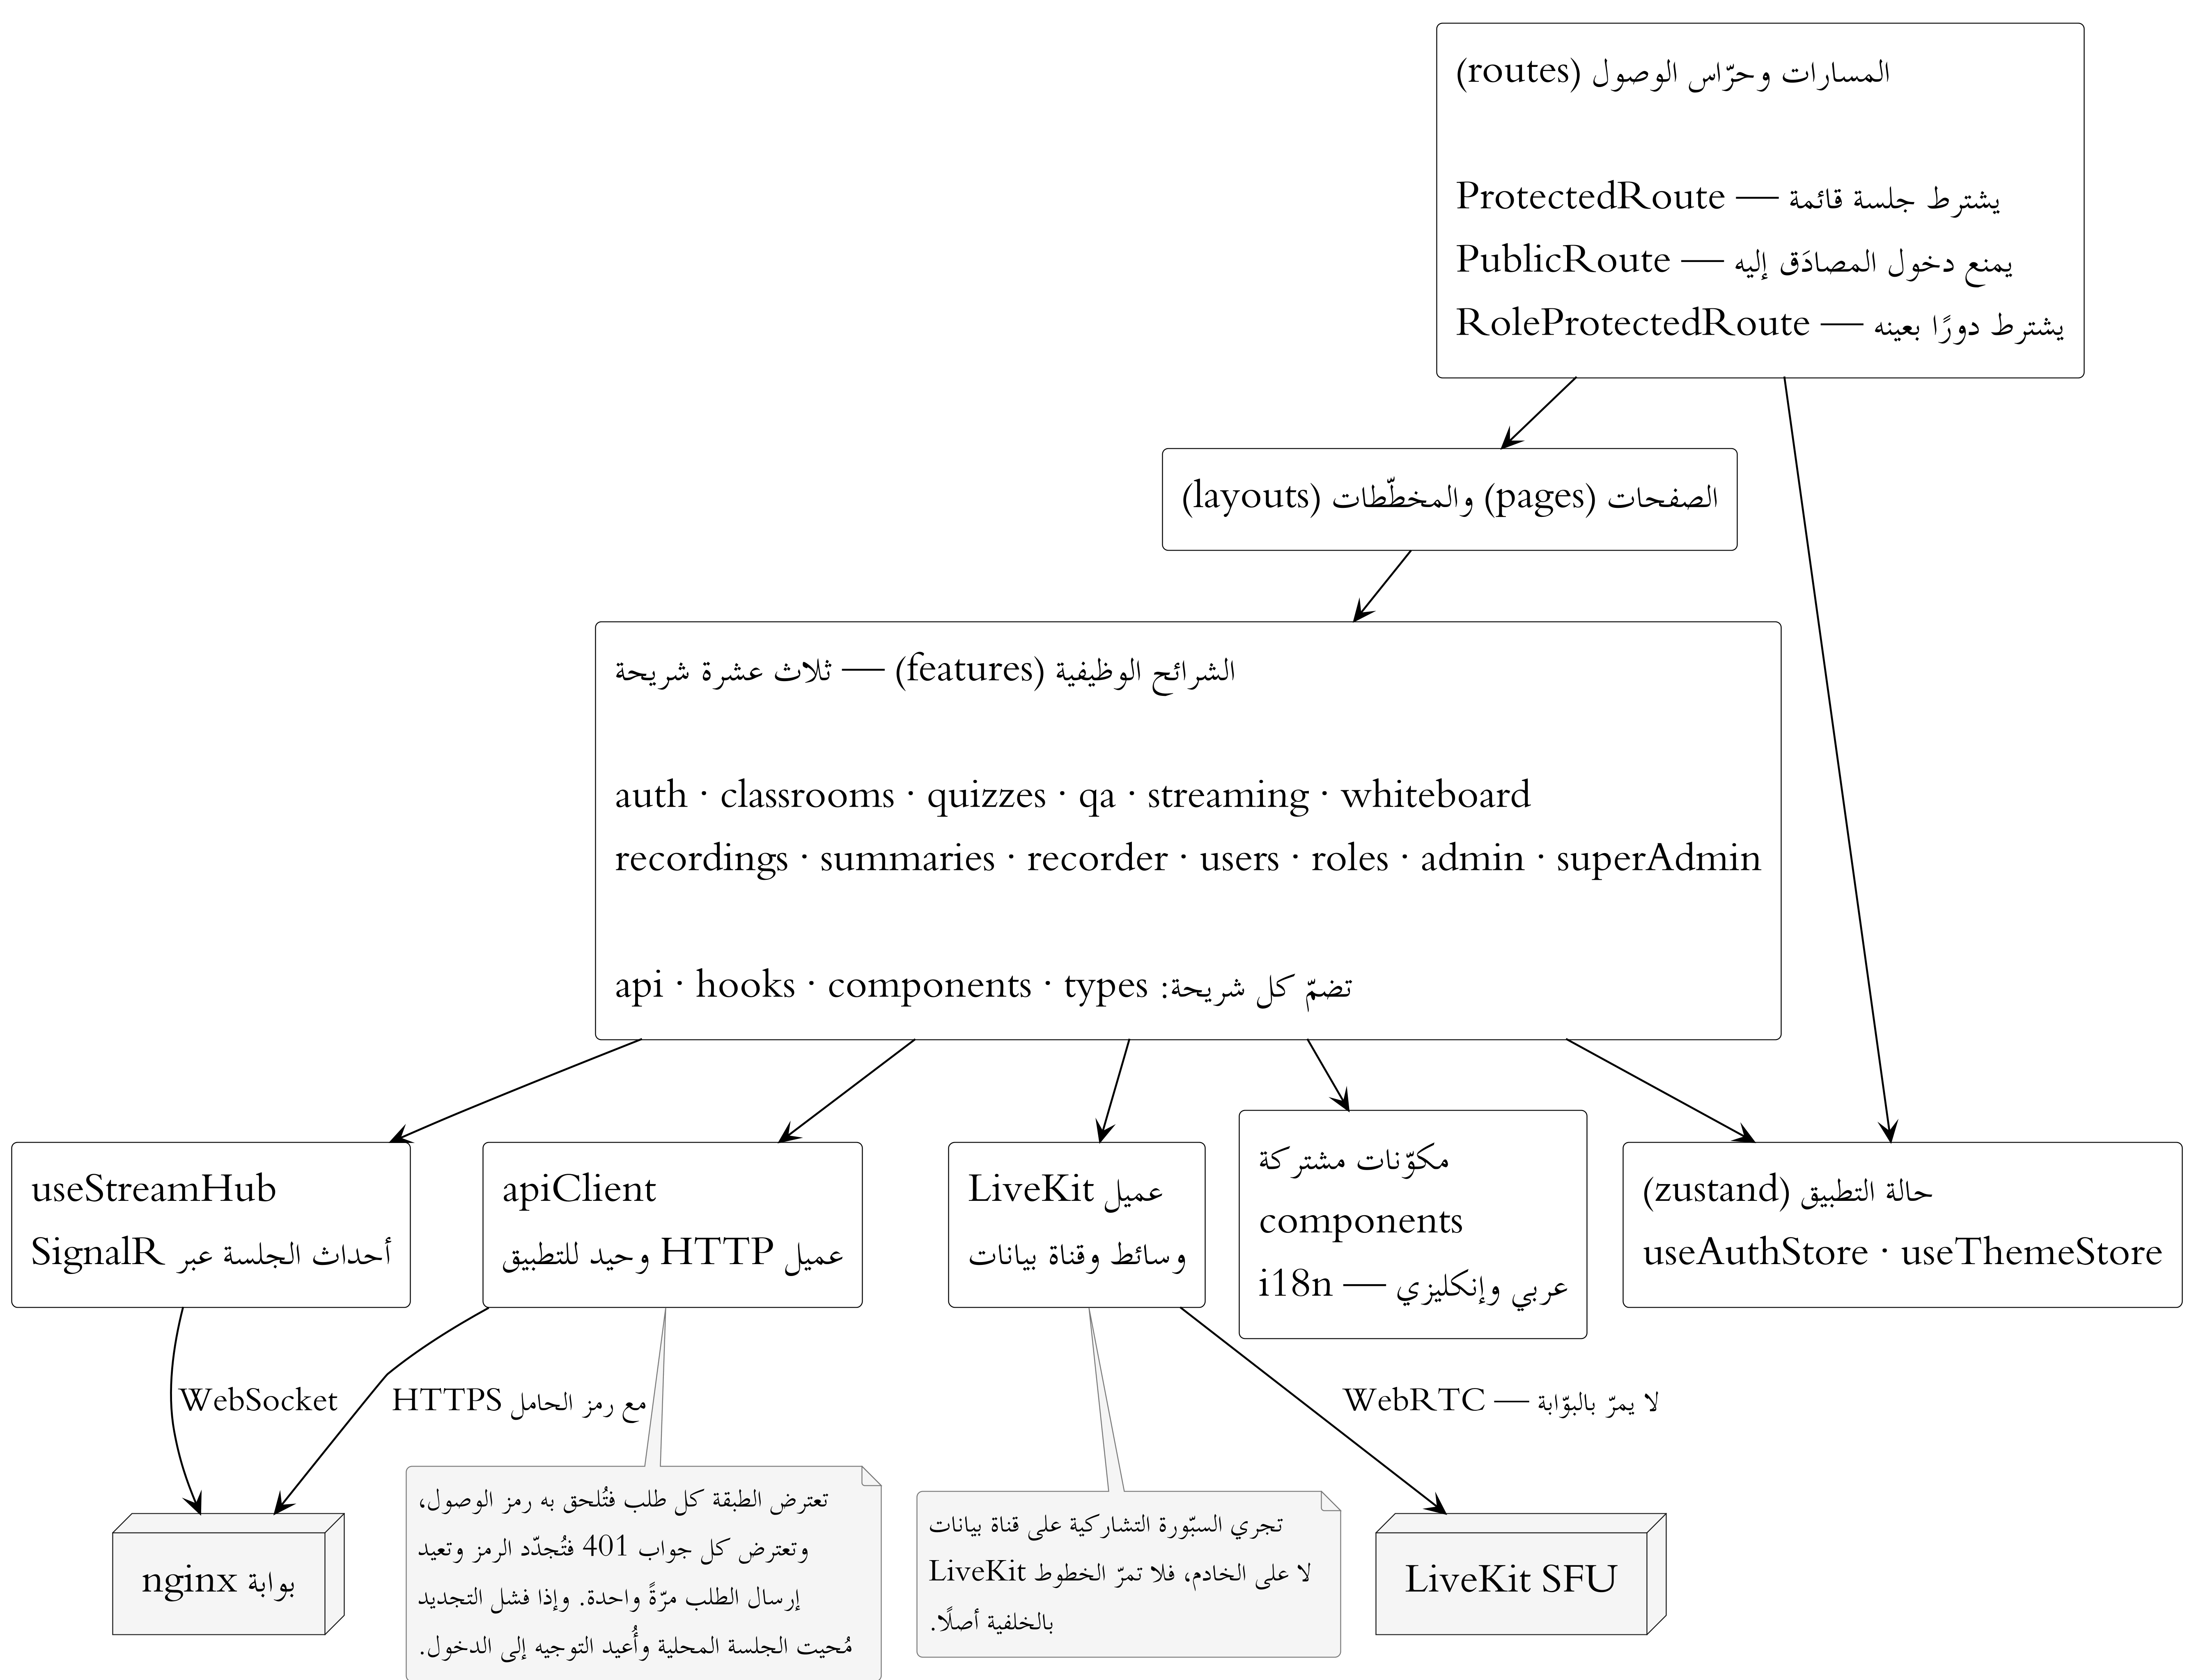
\includegraphics[width=\textwidth,height=0.8\textheight,keepaspectratio]{figures/comp-07-frontend.png}
  \caption{مخطط مكوّنات تطبيق الويب.}
  \label{fig:comp-07}
\end{figure}

ويقوم تصميم التطبيق على أربعة قرارات:

\begin{enumerate}
  \item \textbf{التقسيم بحسب الوظيفة}: تقابل الشرائح الثلاث عشرة مجالاتِ الخدمات الخلفية، فيبقى أثر أيّ تغيير محصورًا في شريحة واحدة. ويقابل التقسيم بحسب الطبقة التقنية ذلك بتوزيع الوظيفة الواحدة على مجلّدات متباعدة.
  \item \textbf{حدّ وحيد للاتصال}: تمرّ نداءات الشرائح كلّها عبر عميل \en{HTTP} واحد هو \en{apiClient}. ويُلحق هذا العميل رمز الوصول بكل طلب، ويعالج الجواب \en{401} بتجديد الرمز وإعادة إرسال الطلب مرّةً واحدة. فإن فشل التجديد محا الجلسة المحلية وأعاد التوجيه إلى صفحة الدخول، دون أن تعلم الشريحة الطالِبة بشيء من ذلك.
  \item \textbf{حراسة على مستوى المسار}: تمنع المكوّنات \en{ProtectedRoute} و\en{PublicRoute} و\en{RoleProtectedRoute} عرض المسارات غير المصرَّح بها للمستخدم الحالي. وهذه الحراسة طبقة إضافية لا حدٌّ أمني، إذ يجري التحقّق الفعلي من الصلاحية في الخدمات الخلفية عند كل طلب.
  \item \textbf{ثلاث قنوات متمايزة}: تُنقَل نداءات \en{REST} وأحداث الجلسة عبر البوّابة العكسية، الأولى فوق \en{HTTPS} والثانية فوق \en{SignalR}. أمّا الوسائط فتُنقَل عبر \en{WebRTC} مباشرةً إلى خادم \en{LiveKit} دون المرور بالبوّابة. وتجري السبّورة التشاركية على قناة بيانات \en{LiveKit} نفسها، فلا تمرّ خطوطها بالخلفية أصلًا.
\end{enumerate}

وتُدار الحالة المشتركة بمخزنَي \en{zustand}: مخزن الجلسة (\en{useAuthStore}) ومخزن السمة (\en{useThemeStore}). وتُدار حالة الخادم في خطّافات كل شريحة بوساطة \en{React Query}. ويدعم التطبيق العربية والإنكليزية عبر \en{i18next} مع تبديل اتجاه الصفحة تبعًا للّغة المختارة.


\section{خدمة إدارة المستخدمين (\en{UserManagementService})}
% Content for Chapter 5, Section 5.4 — pulled in by chapters/05-system-design.tex
\subsection{مكوّنات الخدمة}

% CH2-REF: originally "(\en{Clean Architecture}) الموصوف في القسم~\ref{subsec:clean-architecture}،" — restore with chapter 2.
اتُّبع في تصميم هذه الخدمة، كما في بقية خدمات \en{.NET}، نمطُ المعمارية النظيفة (\en{Clean Architecture})، بأربع طبقات متّحدة المركز تتّجه التبعيات فيها نحو الداخل. ويعرض الشكل~\ref{fig:comp-01} مكوّنات الخدمة موزّعةً على هذه الطبقات مع روابطها الخارجية.

\begin{figure}[htbp]
  \centering
  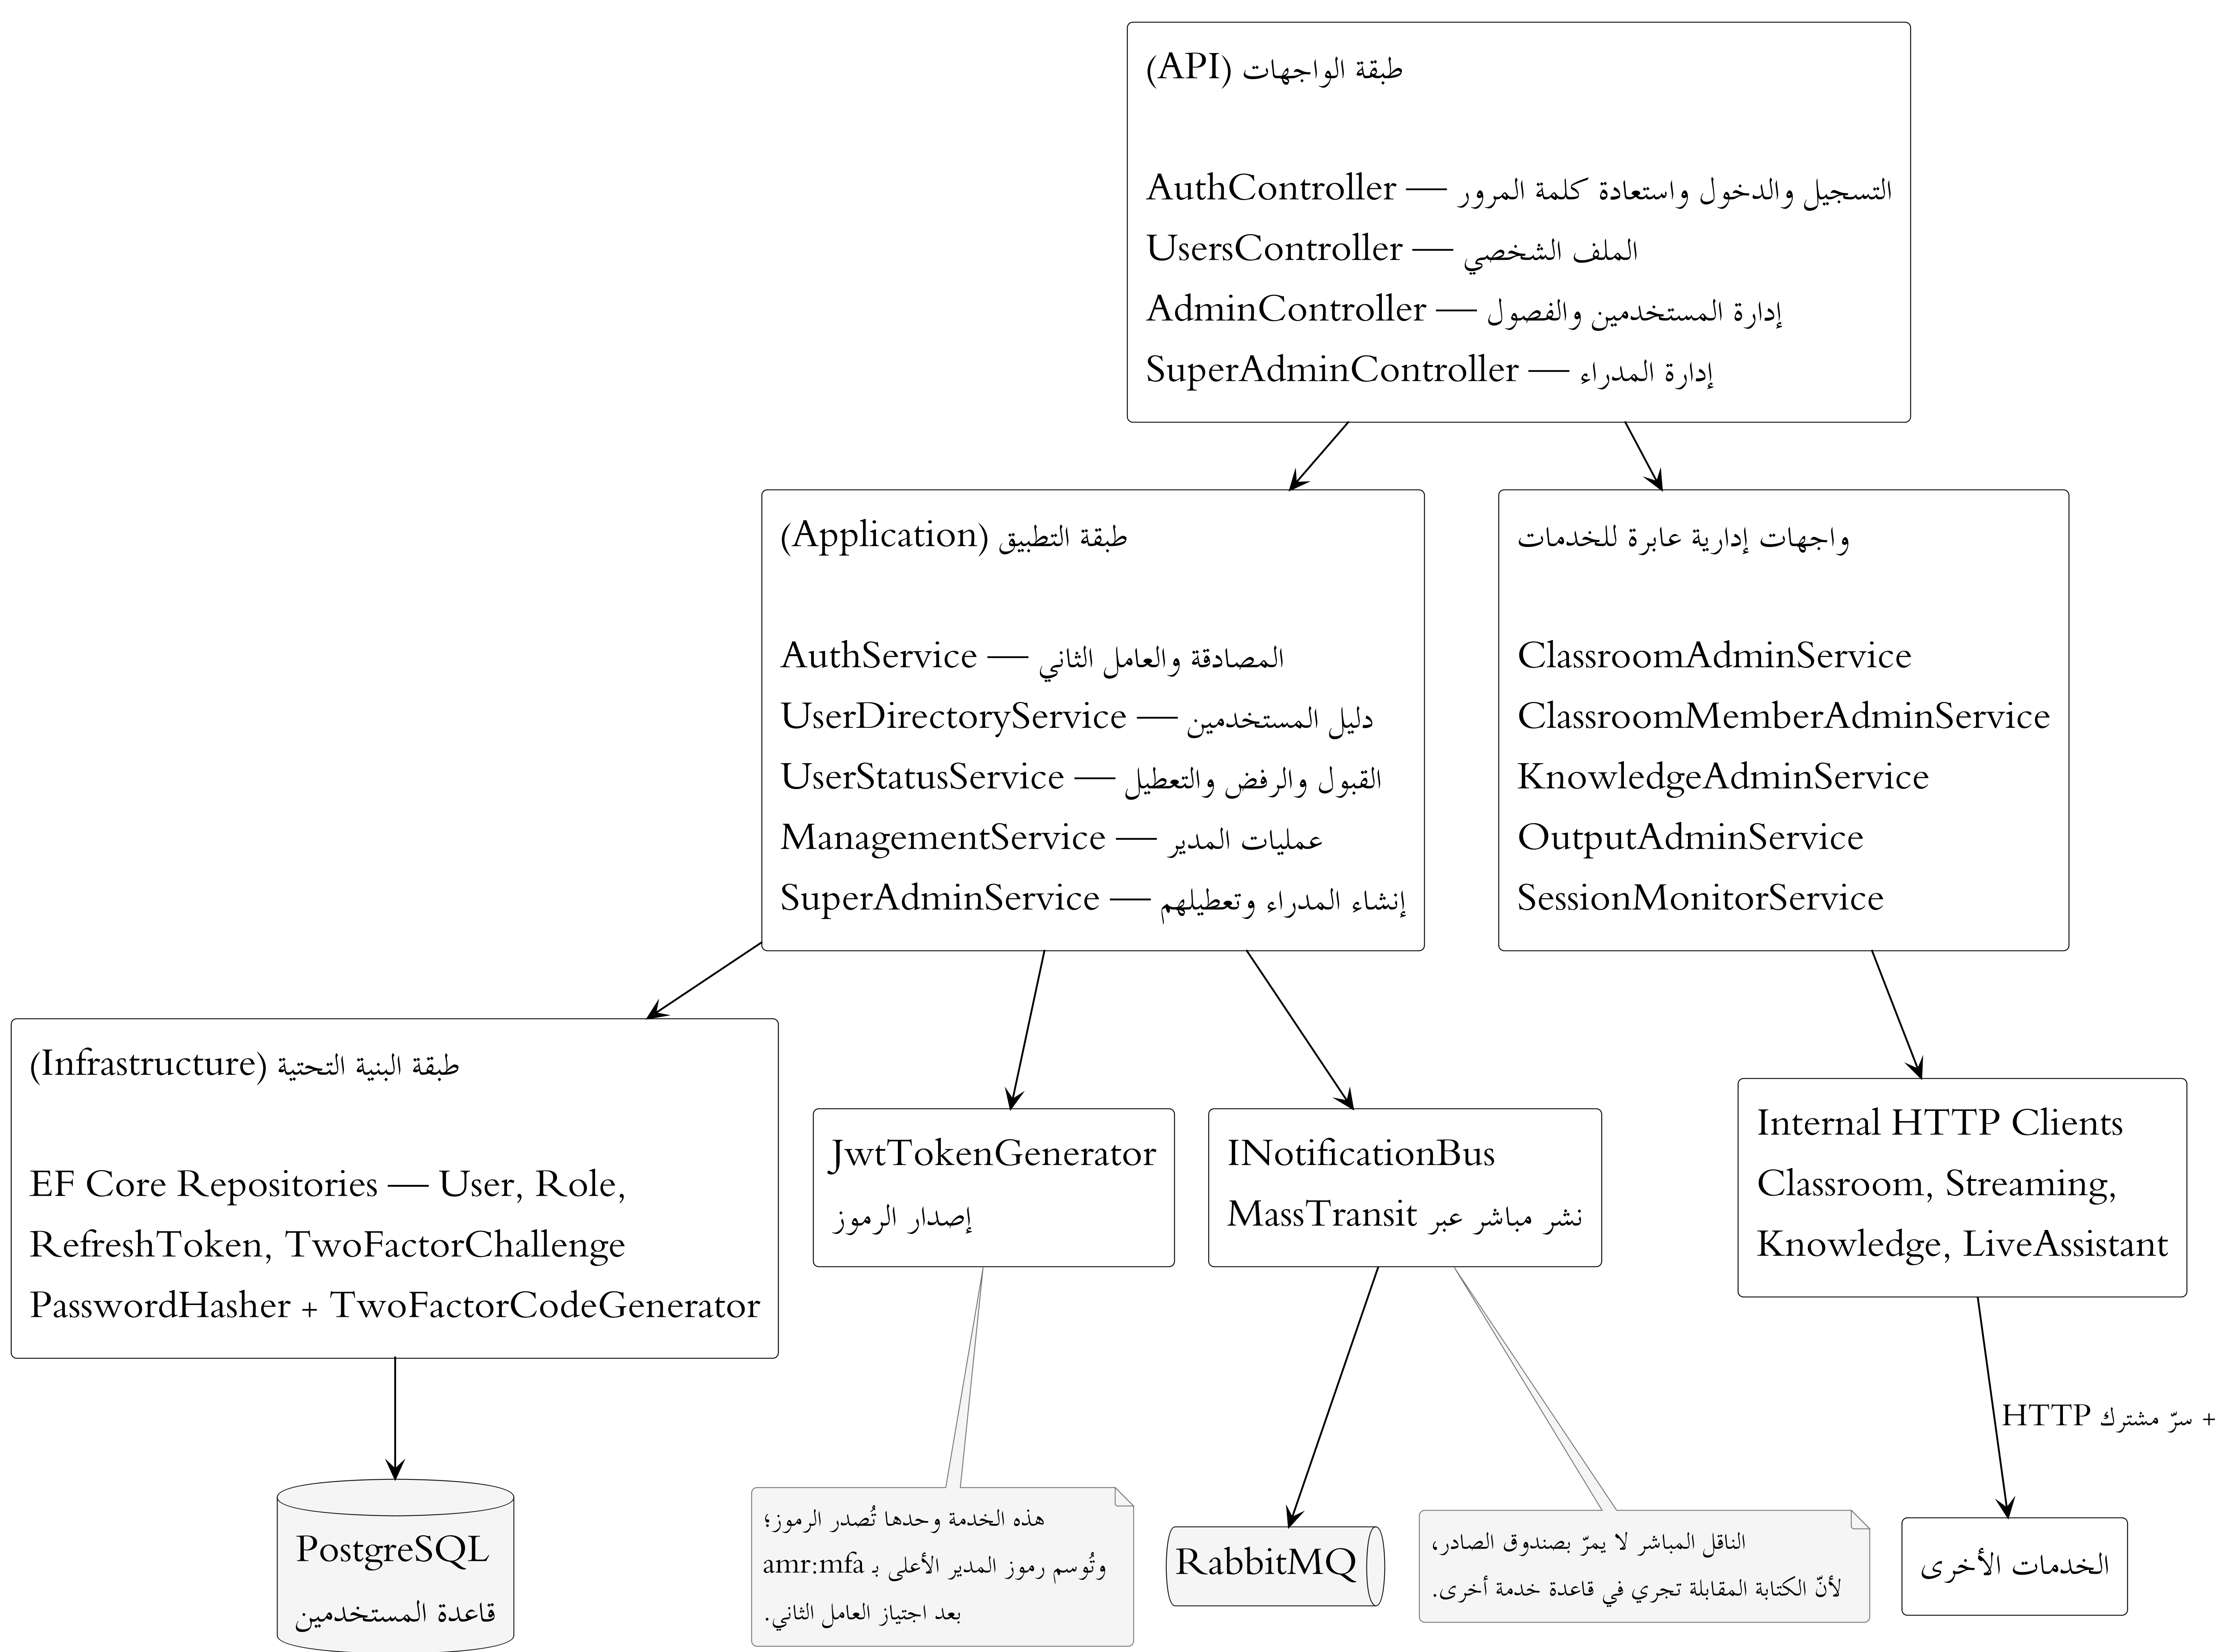
\includegraphics[width=\textwidth,height=0.8\textheight,keepaspectratio]{figures/comp-01-user-management.png}
  \caption{مخطط المكوّنات التفصيلي لخدمة إدارة المستخدمين.}
  \label{fig:comp-01}
\end{figure}

وتتّصل الخدمة بمحيطها عبر ثلاثة مسارات:

\begin{enumerate}
  \item \textbf{مولّد الرموز} (\en{JwtTokenGenerator}): تنفرد هذه الخدمة بإصدار رموز الوصول، بينما تكتفي بقية الخدمات بالتحقّق منها. ويحصر هذا التمركز أيّ تعديل على سياسة المصادقة في موضع واحد.
  \item \textbf{ناقل الإشعارات} (\en{INotificationBus}): يُستعمل لنشر ما يتطلّب تنفيذ إجراء في خدمة أخرى، كإرسال رمز العامل الثاني أو الإعلام بتغيّر حالة مستخدم.
  \item \textbf{عملاء \en{HTTP} الداخليون}: تستعملهم الواجهات الإدارية العابرة للخدمات، إذ يحتاج المدير الأعلى إلى الاطّلاع على الفصول والجلسات والمخرجات المملوكة لخدمات أخرى والتصرّف بها.
\end{enumerate}

ويُستعمل ناقل الإشعارات هنا بصيغته المباشرة، دون صندوق الصادر المعتمد في خدمة الفصول. ويقتضي نمط صندوق الصادر أن تجري الكتابة المقابلة في القاعدة نفسها وضمن المعاملة نفسها، وهو شرط لا يتحقّق حين يكون أثر الرسالة في قاعدة خدمة أخرى.

\subsection{نموذج البيانات}

يقوم نموذج بيانات الخدمة على خمسة كيانات يعرضها الشكل~\ref{fig:erd-01}: المستخدم (\en{users}) والدور (\en{roles})، ورموز التحديث (\en{refresh\_tokens})، ورموز استعادة كلمة المرور (\en{reset\_password\_tokens})، وتحدّيات العامل الثاني (\en{two\_factor\_challenges}).

\begin{figure}[htbp]
  \centering
  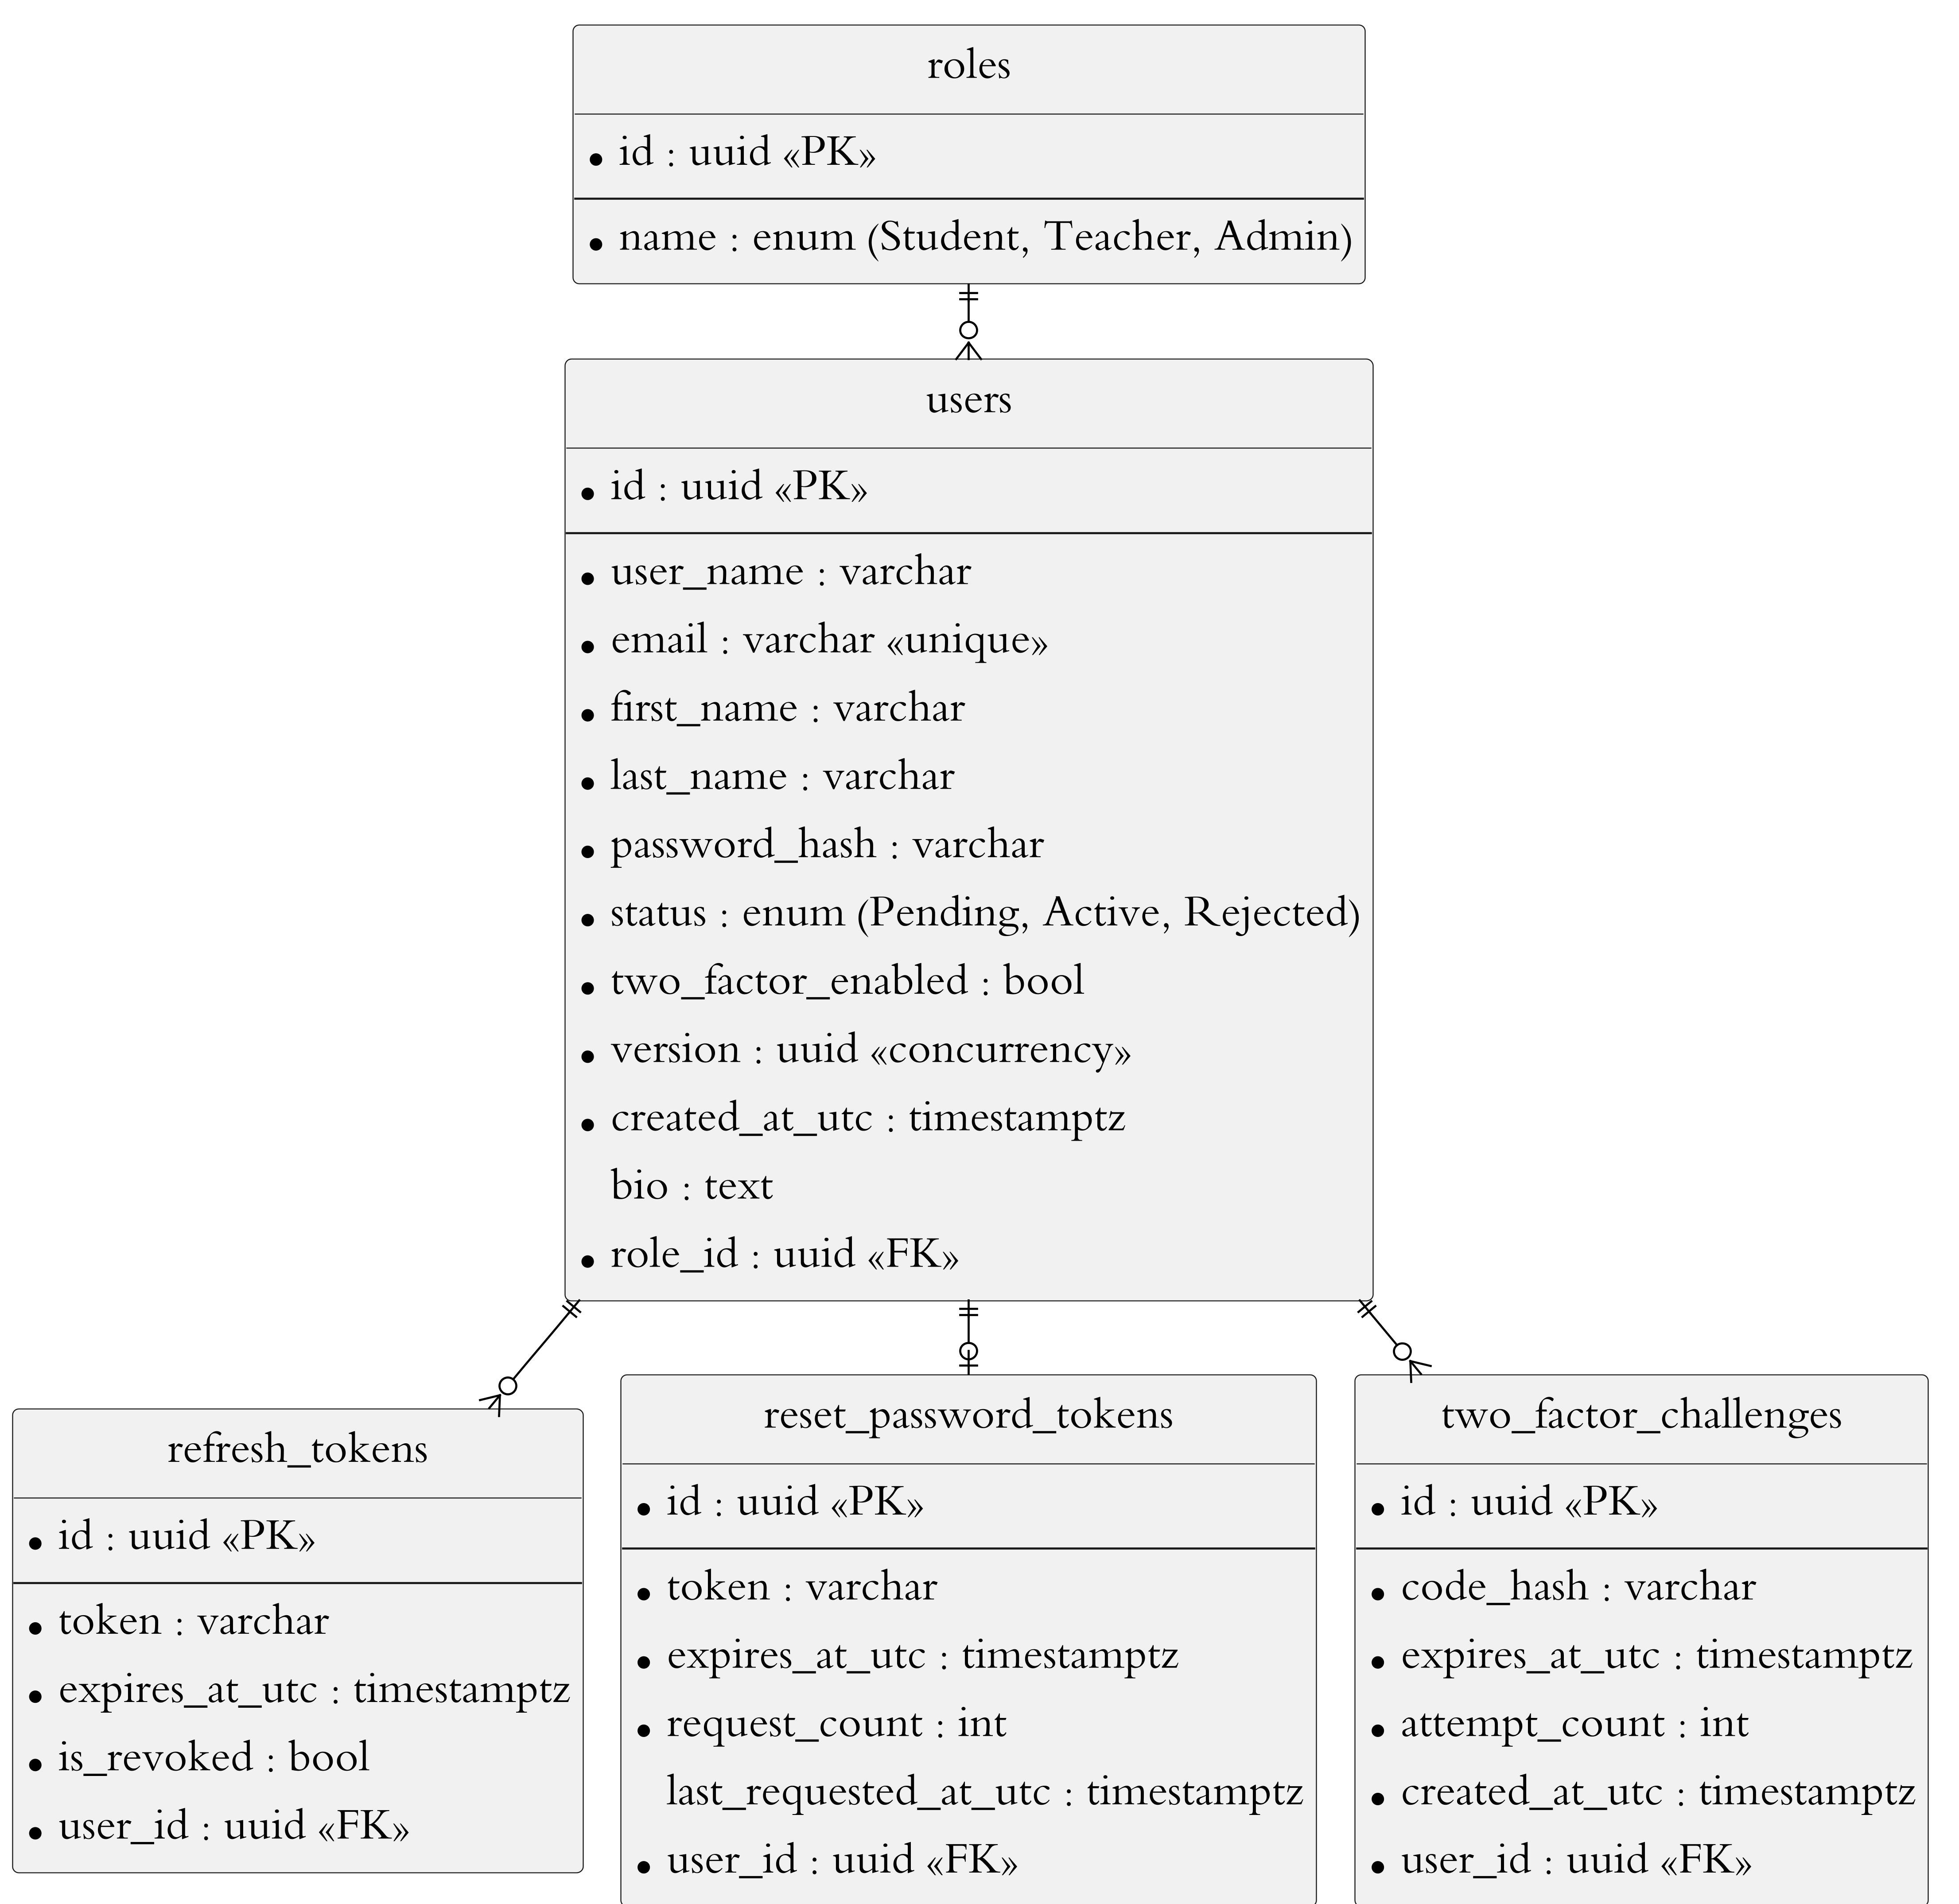
\includegraphics[width=\textwidth,height=0.8\textheight,keepaspectratio]{figures/erd-01-user-management.png}
  \caption{مخطط الكيانات والعلاقات لخدمة إدارة المستخدمين.}
  \label{fig:erd-01}
\end{figure}

وتُخزَّن الرموز الحسّاسة، وهي رمز الاستعادة ورمز العامل الثاني، على هيئة بصمات لا نصوص صريحة. ولا يمنح تسريب قاعدة البيانات عندئذٍ رمزًا صالحًا للاستعمال.

ويُبيَّن تدفّق تسجيل دخول المدير الأعلى بمرحلتيه، وما يقوم عليه من ضوابط أمنية، في القسم~\ref{subsubsec:flow-super-admin-login}.


\section{خدمة الفصول الدراسية (\en{ClassroomService})}
% Content for Chapter 5, Section 5.5 — pulled in by chapters/05-system-design.tex
\subsection{مكوّنات الخدمة}

تضمّ هذه الخدمة ثماني عشرة خدمة تطبيقية، وهي أكبر خدمات النظام حجمًا. ويعرضها الشكل~\ref{fig:comp-02} مجمّعةً بحسب المسؤولية التي تملكها كل مجموعة.

\begin{figure}[htbp]
  \centering
  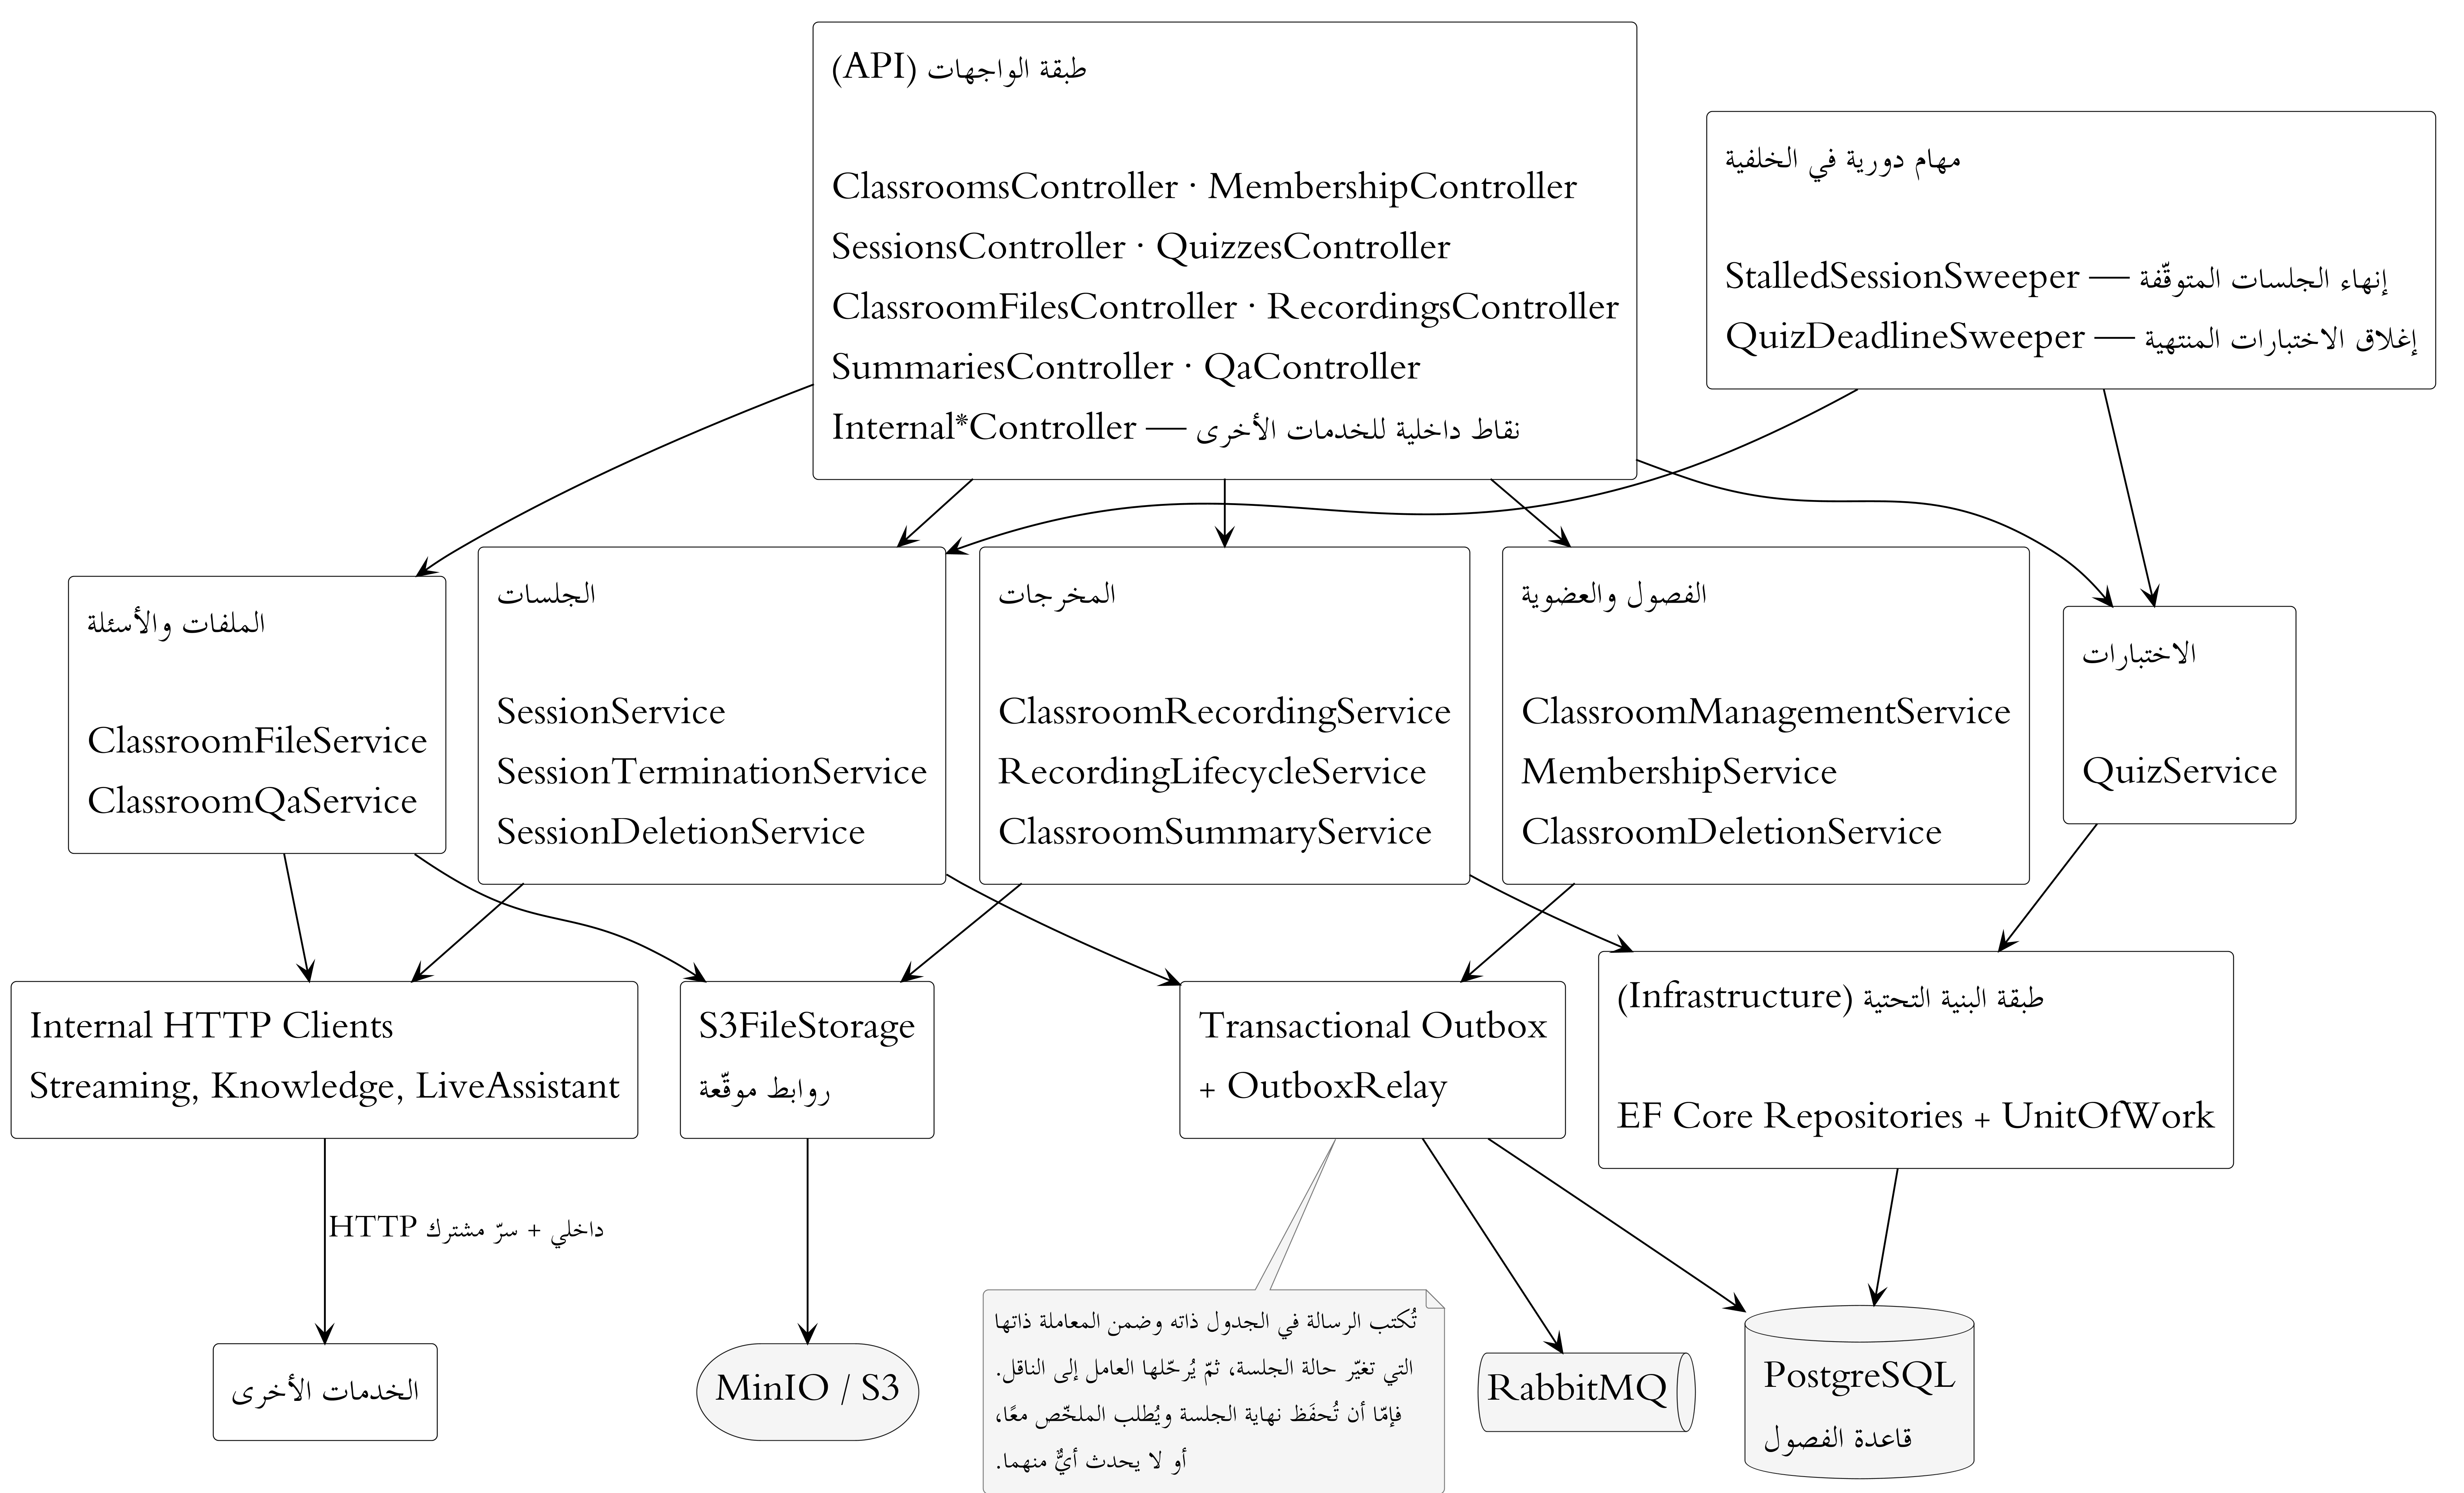
\includegraphics[width=\textwidth,height=0.8\textheight,keepaspectratio]{figures/comp-02-classroom.png}
  \caption{مخطط المكوّنات التفصيلي لخدمة الفصول الدراسية.}
  \label{fig:comp-02}
\end{figure}

وتظهر المهام الدورية في الخلفية منفصلةً عن بقية المكوّنات، لأنّها لا تُستدعى من أيّ مكوّن آخر بل تعمل على مؤقّتات. وتتولّى هذه المهام تصحيح الحالات الشاذّة، كانقطاع اتصال المعلّم في أثناء الجلسة أو انقضاء موعد إغلاق اختبار.

وترتبط هذه الخدمة بمحيطها عبر ثلاثة مسارات:

\begin{enumerate}
  \item \textbf{صندوق الصادر}: تنشر عبره أحداث المجال إلى الناقل.
  \item \textbf{مخزن الملفّات}: تحفظ فيه المواد المرجعية ومخرجات الجلسات، وتُصدر منه روابط موقَّعة محدودة المدّة.
  \item \textbf{عملاء \en{HTTP} الداخليون}: تُشغّل بهم الفهرسة في خدمة المعرفة، وتفكيك الغرف في خدمة البث، وتوليد الاختبارات في خدمة المساعد الحيّ.
\end{enumerate}

\subsection{نموذج البيانات}

يضمّ نموذج بيانات الخدمة اثني عشر كيانًا يعرضها الشكل~\ref{fig:erd-02}، موزّعةً على أربع مجموعات: الفصول وملفّاتها وعضويّاتها، والجلسات، ومخرجات الجلسات من تسجيلات وملخّصات، والاختبارات وهي المجموعة الأكبر.

\begin{figure}[htbp]
  \centering
  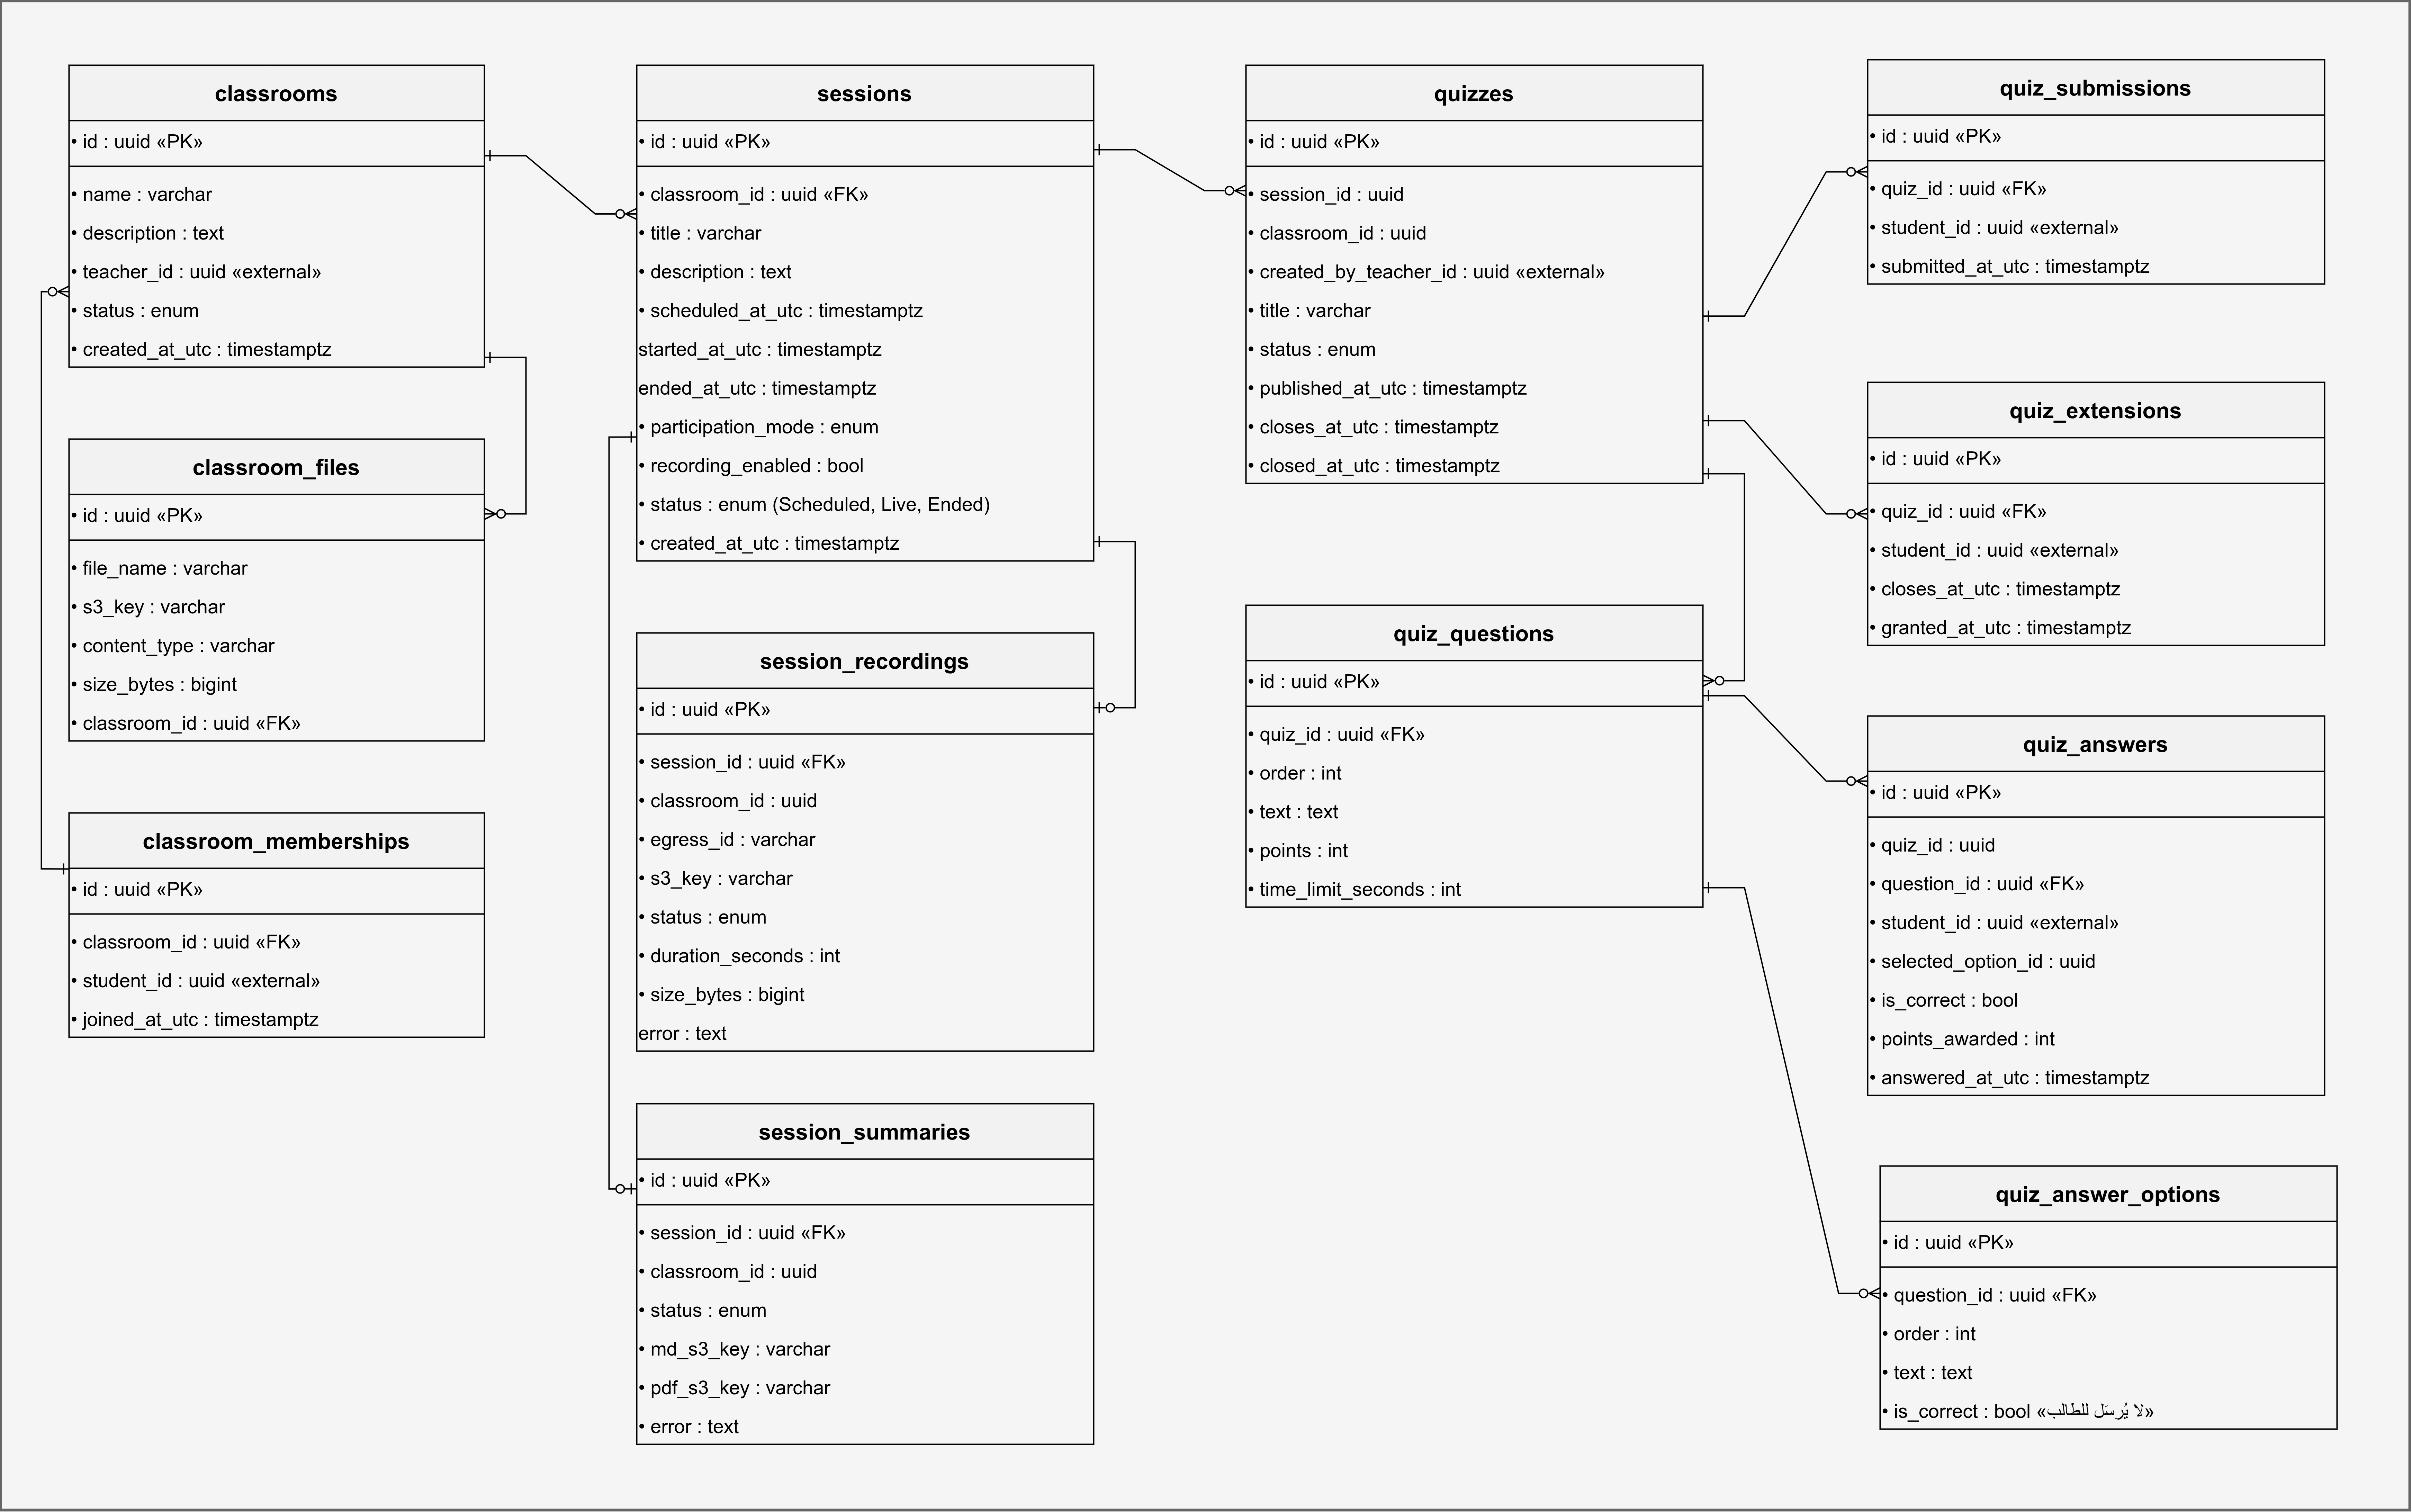
\includegraphics[width=\textwidth,height=0.8\textheight,keepaspectratio]{figures/erd-02-classroom.png}
  \caption{مخطط الكيانات والعلاقات لخدمة الفصول الدراسية.}
  \label{fig:erd-02}
\end{figure}

ويعرض الشكل~\ref{fig:class-02} تصميم تجميعة الاختبار (\en{Quiz Aggregate}) بمزيد من التفصيل.

\begin{figure}[htbp]
  \centering
  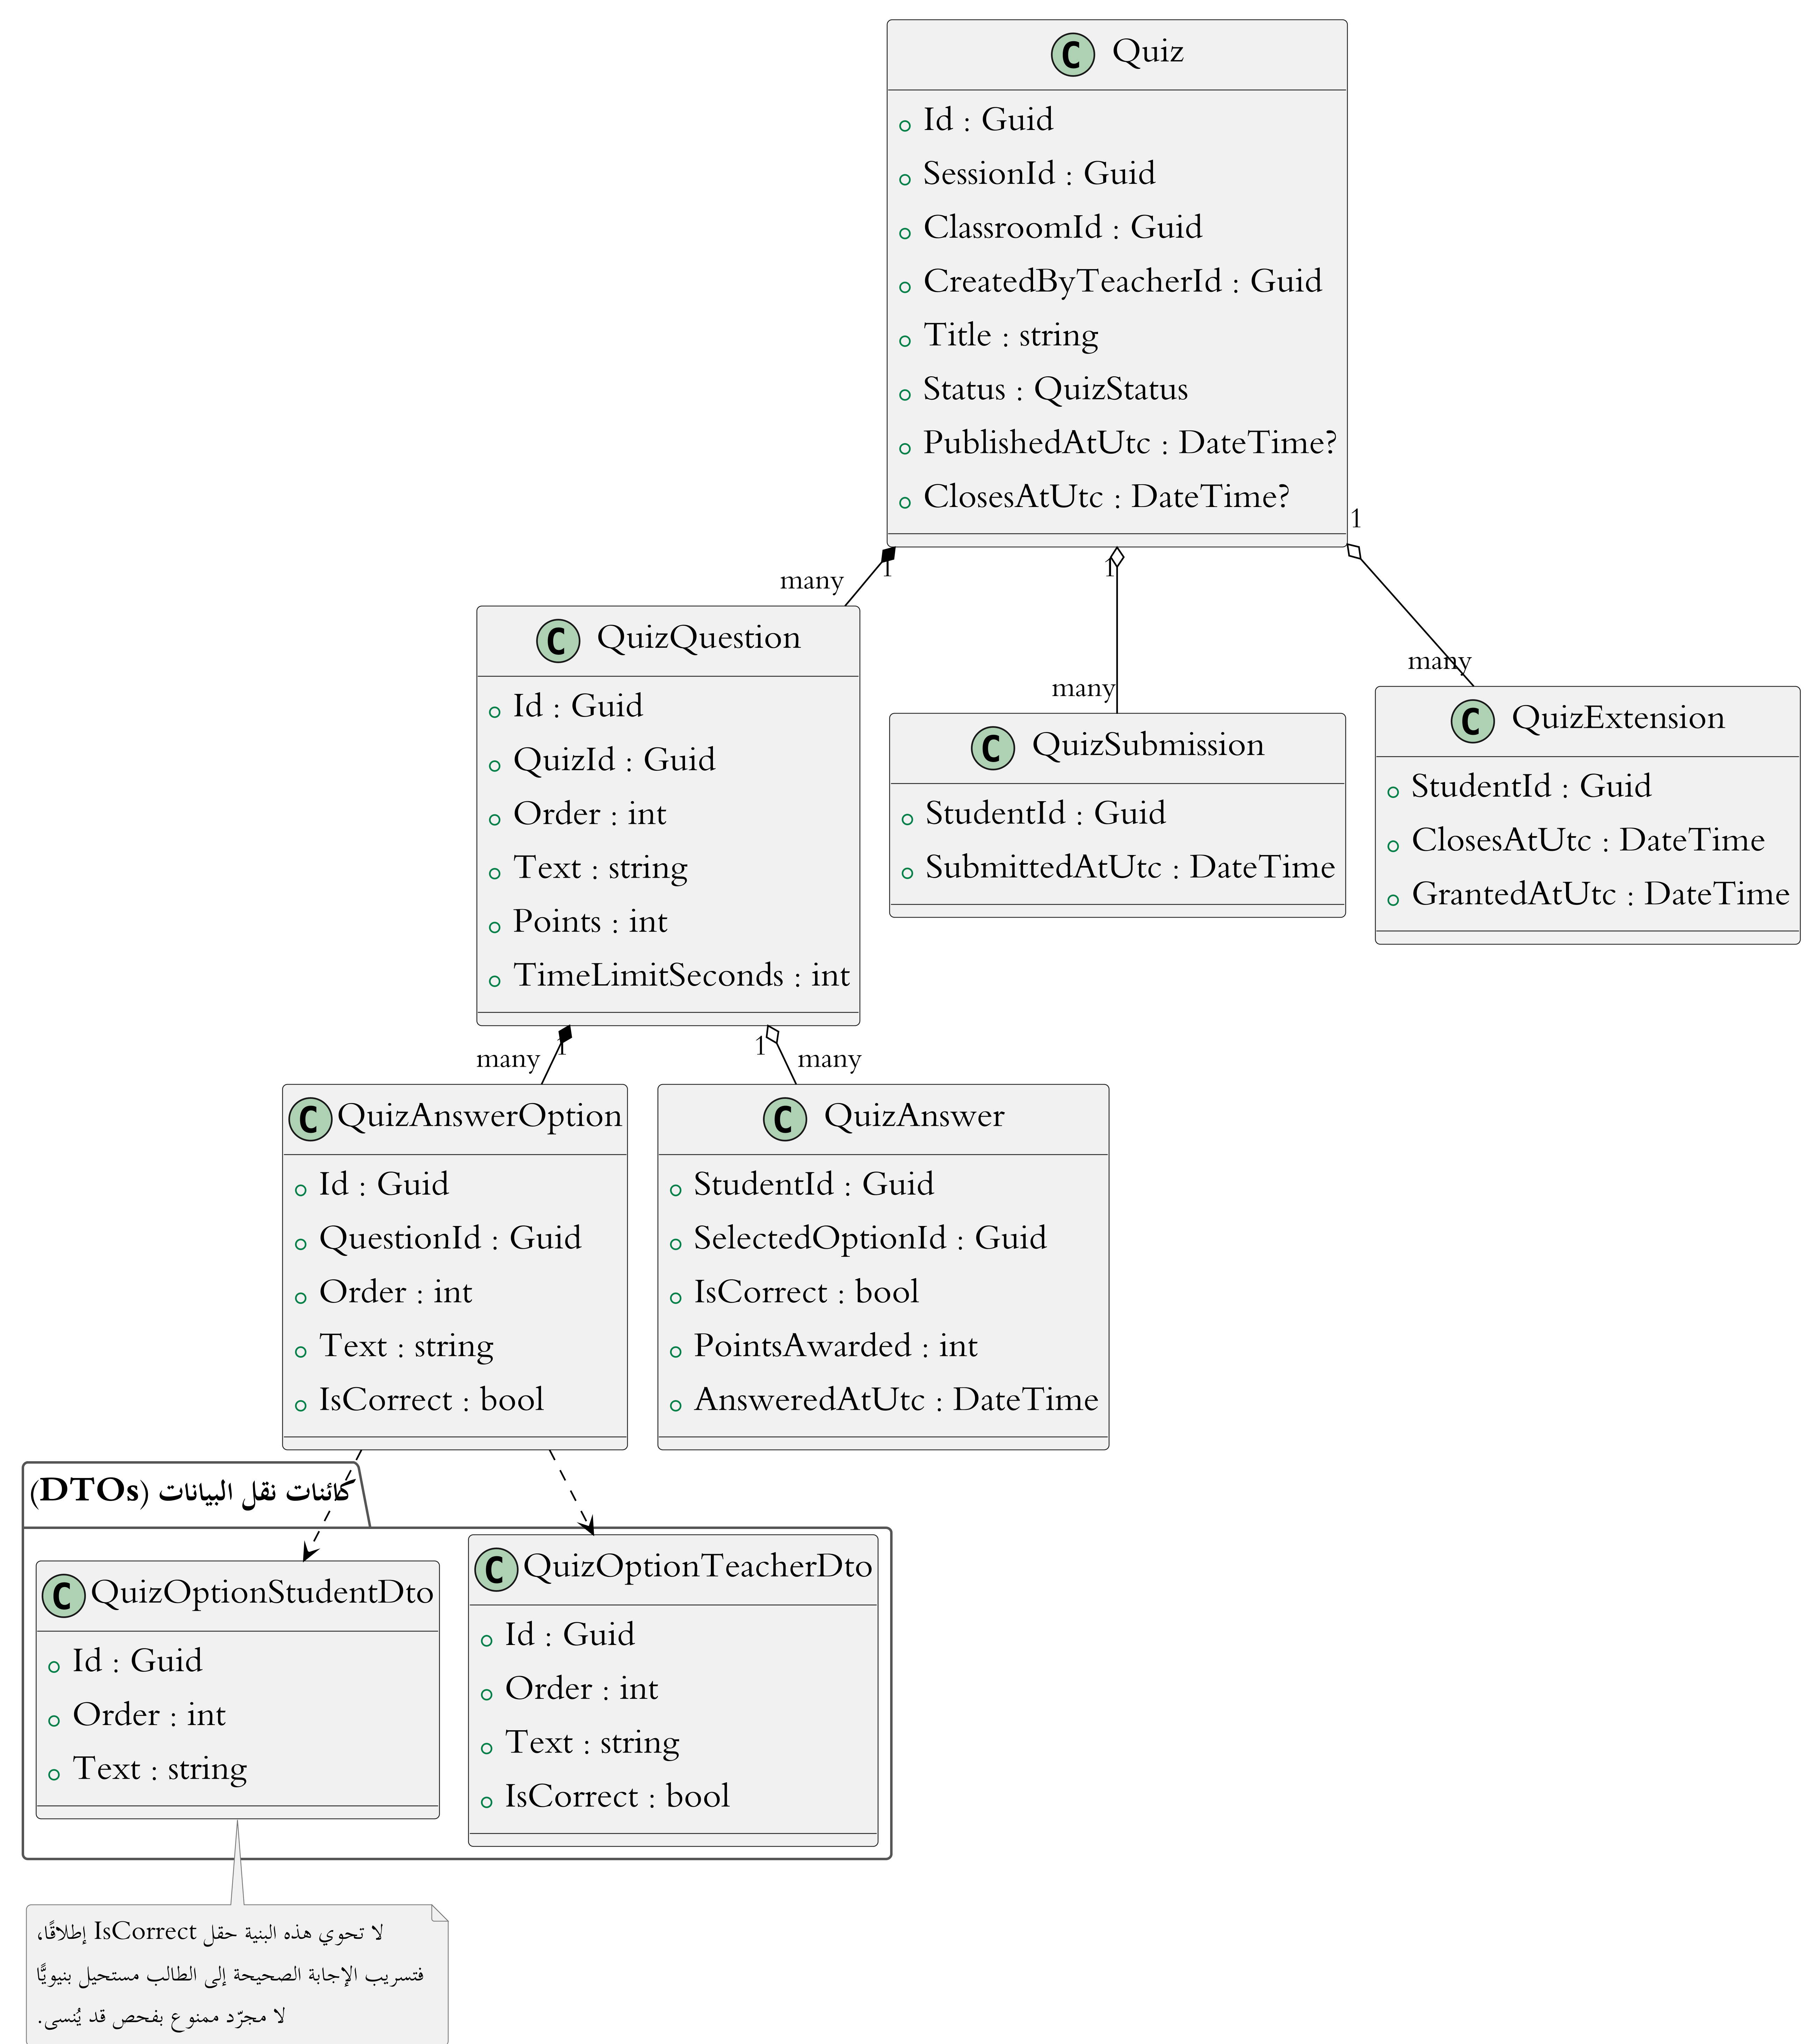
\includegraphics[width=\textwidth,height=0.8\textheight,keepaspectratio]{figures/class-02-quiz-domain.png}
  \caption{مخطط الصفوف لتجميعة الاختبار في خدمة الفصول الدراسية.}
  \label{fig:class-02}
\end{figure}

ويُحفظ الخيار الصحيح لكل سؤال في الحقل \en{IsCorrect} ضمن الكيان \en{QuizAnswerOption}. ولمنع وصول هذا الحقل إلى الطالب، عُرّفت بنيتان منفصلتان لنقل البيانات: بنية للمعلّم تتضمّن الحقل، وبنية للطالب لا تتضمّنه. ويمنع هذا الفصل البنيوي تسريب الإجابة الصحيحة، خلافًا للفحص البرمجي الذي قد يُغفَل عند إضافة مسار جديد.

ويُبيَّن تدفّق إنهاء الجلسة الحيّة، وما يعالجه من مشكلات السباق والذرّية والترتيب، في القسم~\ref{subsubsec:flow-session-end}.


\section{خدمة البث (\en{StreamingService})}
% Content for Chapter 5, Section 5.6 — pulled in by chapters/05-system-design.tex
\subsection{مكوّنات الخدمة}

تضمّ طبقة التطبيق في هذه الخدمة خدمة واحدة، ويقع معظم التعقيد في طبقة البنية التحتية، لأن التسجيل عملية يقودها نظام خارجي يُجيب لاحقاً بإشعار غير مضمون الوصول. ويعرض الشكل~\ref{fig:comp-03} مكوّنات الخدمة وروابطها الخارجية.

\begin{figure}[htbp]
  \centering
  % 2.20:1 — full width is ~30% of the text block, so it places inline.
  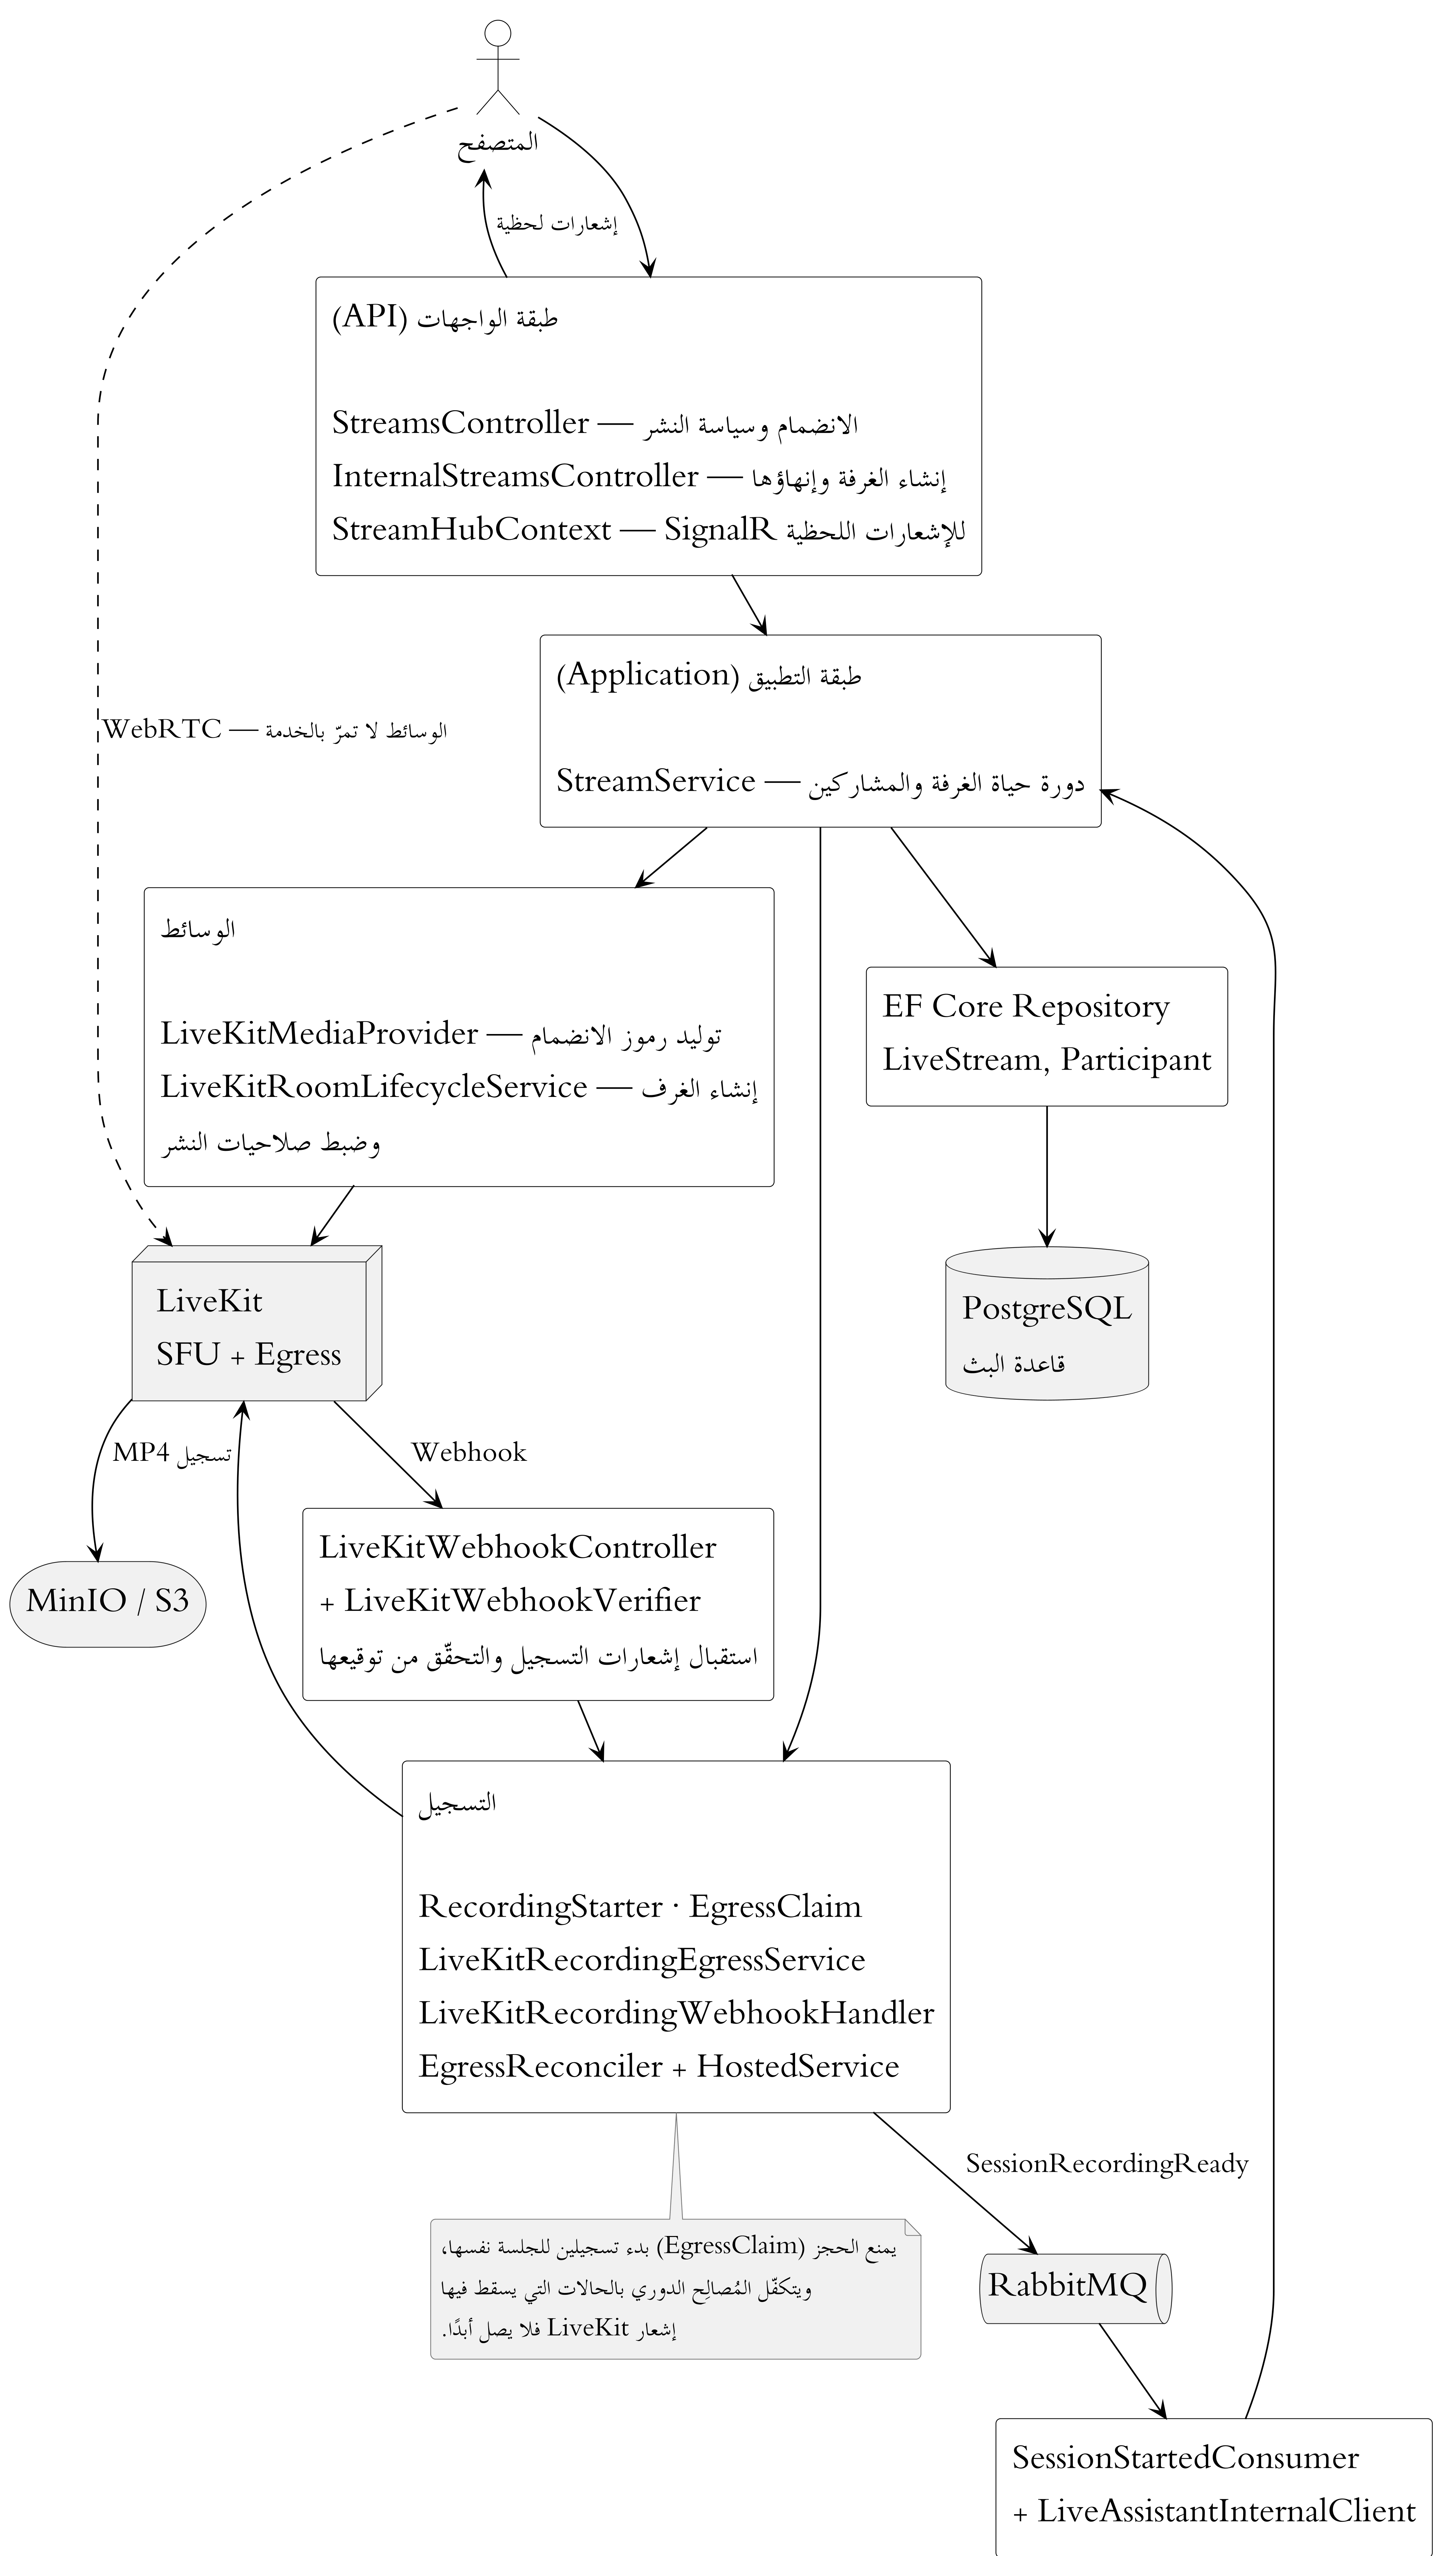
\includegraphics[width=\textwidth,height=0.8\textheight,keepaspectratio]{figures/comp-03-streaming.png}
  \caption{مخطط مكوّنات خدمة البث.}
  \label{fig:comp-03}
\end{figure}

ولا تمرّ الوسائط بالخدمة؛ إذ يتّصل المتصفّح بخادم \en{LiveKit} مباشرة عبر \en{WebRTC}، وتقتصر مهمّة الخدمة على إصدار رمز انضمام محدود الصلاحيات يحدّد ما يُسمح لصاحبه بنشره من صوت وصورة. ويمنع هذا الفصل تحوّل الخدمة إلى عنق زجاجة عند ارتفاع عدد المشاركين.

\subsection{نموذج البيانات}

يضمّ نموذج البيانات خمسة كيانات يعرضها الشكل~\ref{fig:erd-03}: البثّ الحيّ ومشاركوه، ورسائل المحادثة والأسئلة والتفاعلات المرافقة للجلسة.

% [H]: pinned under the paragraph that introduces it. Portrait at 0.90:1, so
% full width would be ~79% of the text block and could not share the page.
\begin{figure}[H]
  \centering
  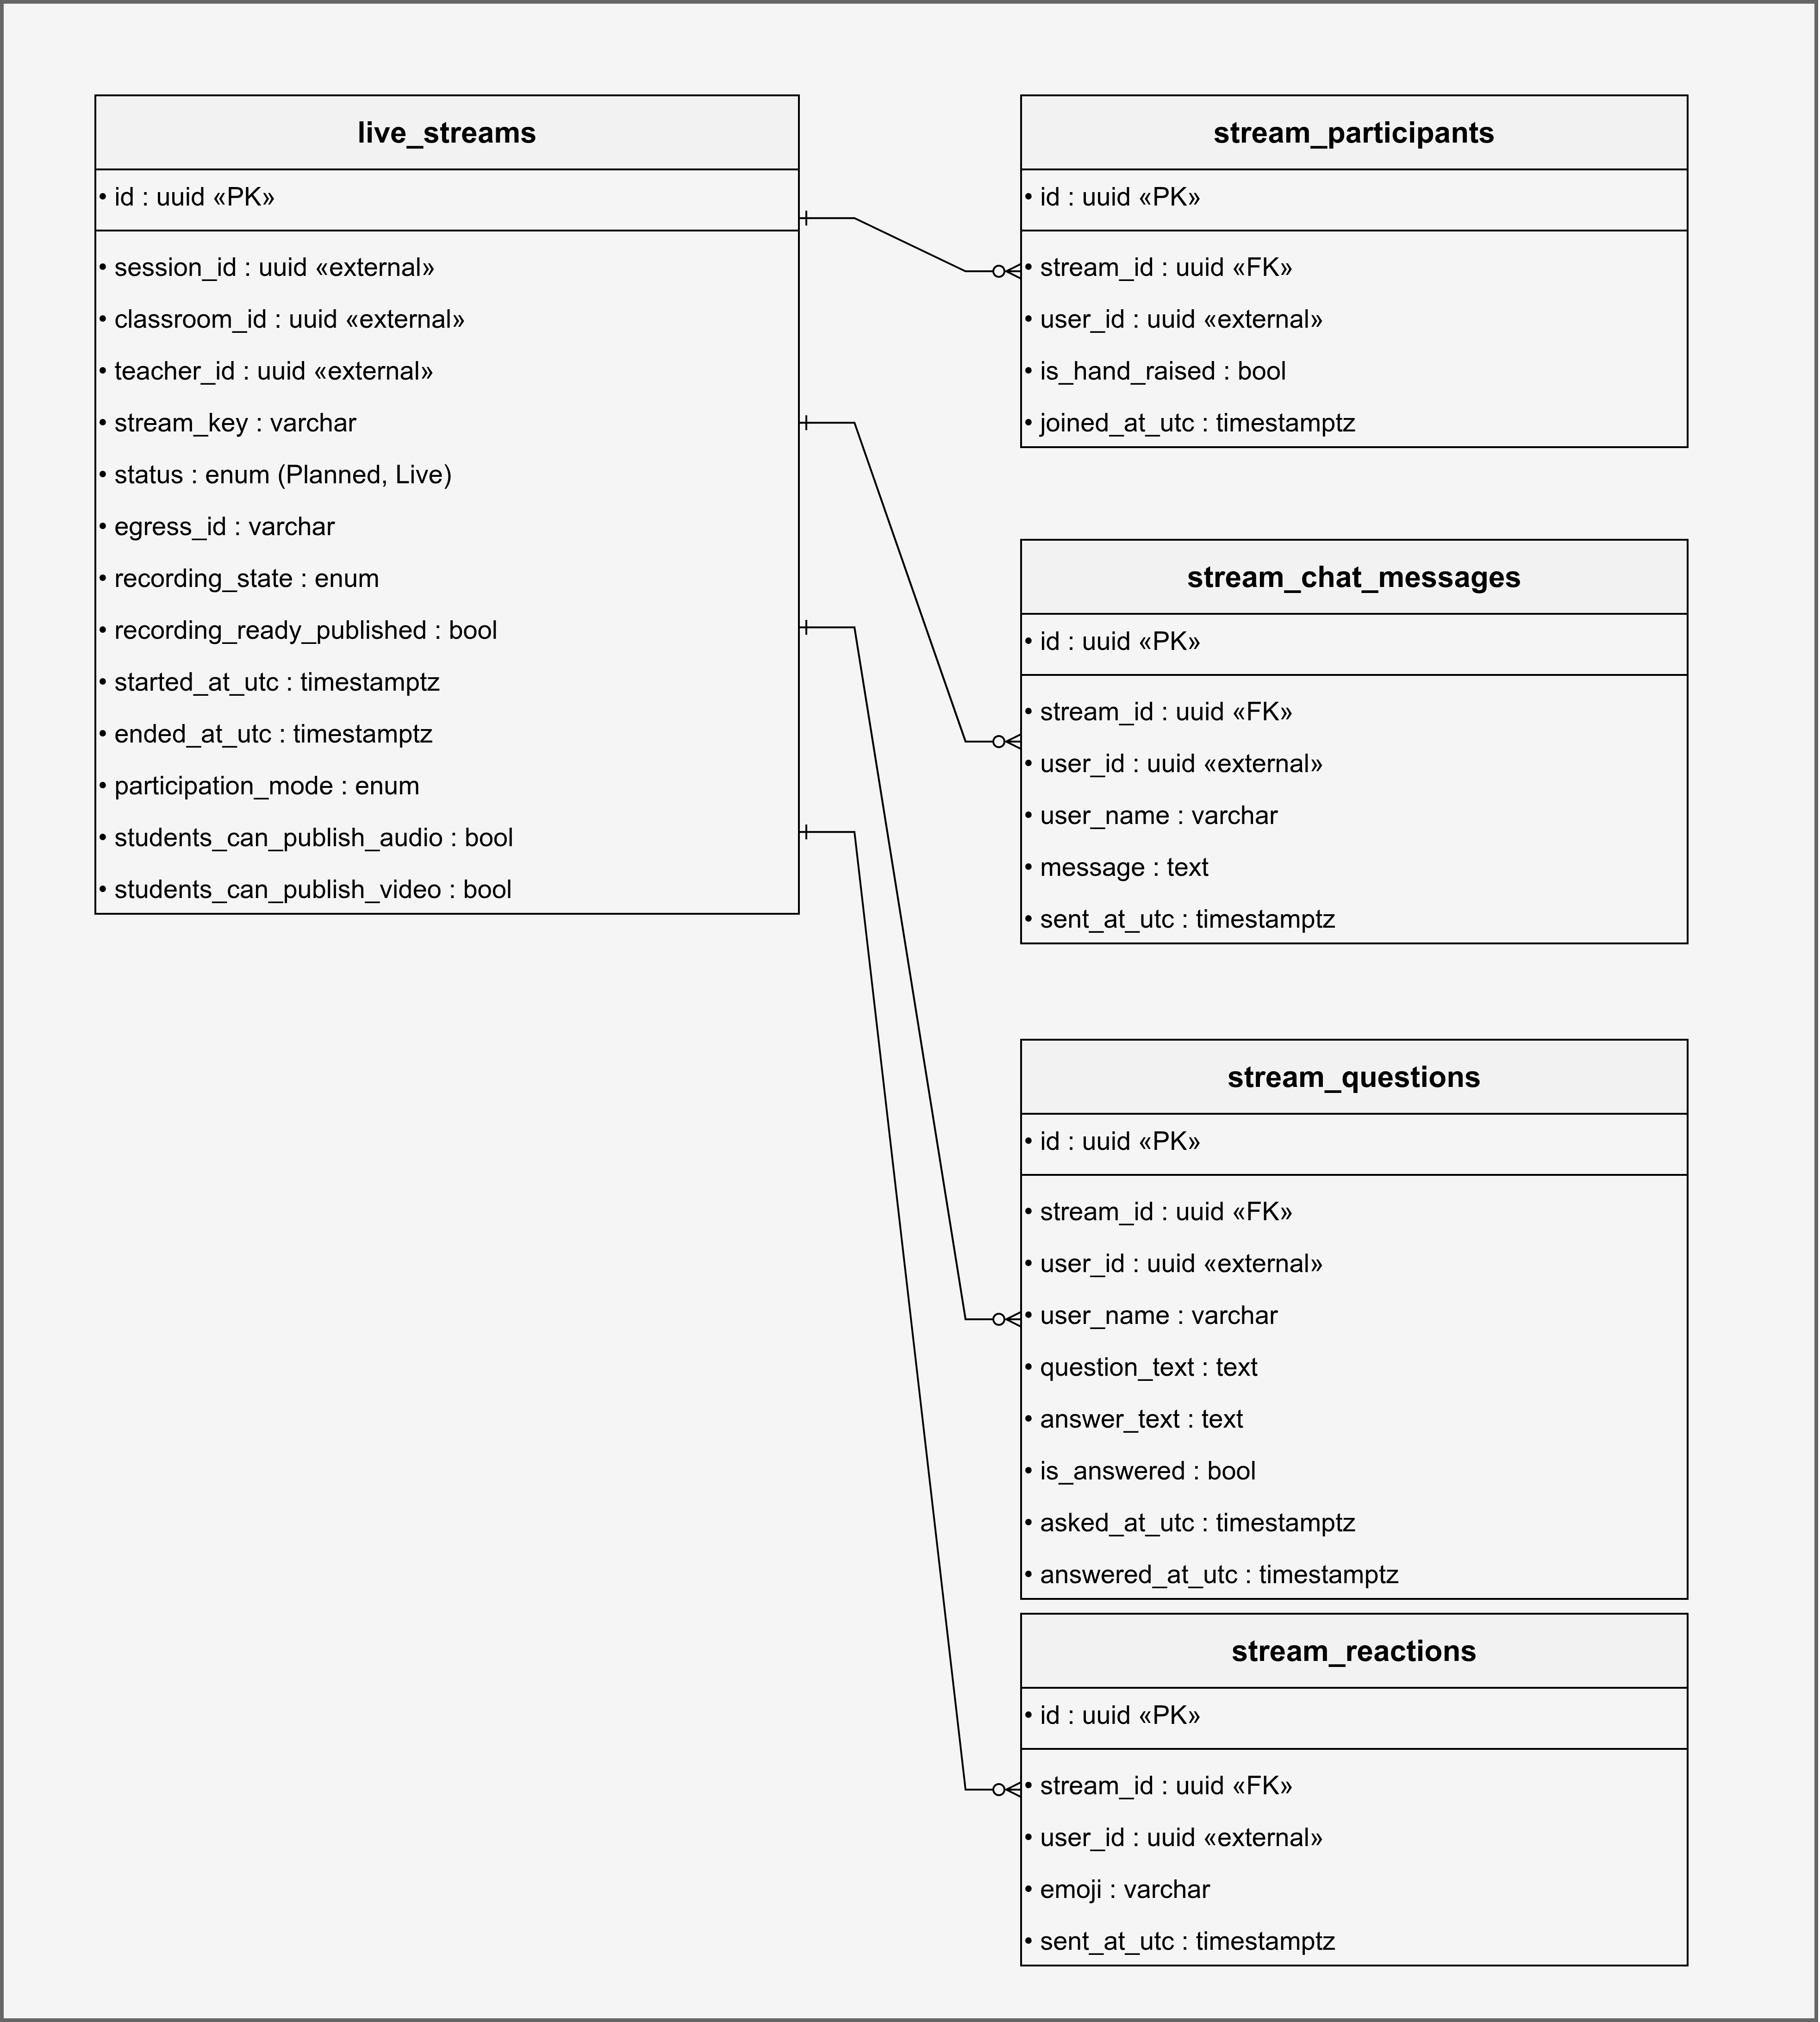
\includegraphics[width=0.55\textwidth,height=0.8\textheight,keepaspectratio]{figures/erd-03-streaming.png}
  \caption{مخطط الكيانات والعلاقات لخدمة البث.}
  \label{fig:erd-03}
\end{figure}


\section{خدمة البريد (\en{EmailService})}
% Content for Chapter 5, Section 5.7 — pulled in by chapters/05-system-design.tex
\subsection{مكوّنات الخدمة}

هي الخدمة الوحيدة في النظام التي لا تملك قاعدة بيانات ولا واجهة \en{HTTP} واردة، فهي مستهلِكة صرفة. ويعرض الشكل~\ref{fig:comp-04} مكوّناتها.

\begin{figure}[htbp]
  \centering
  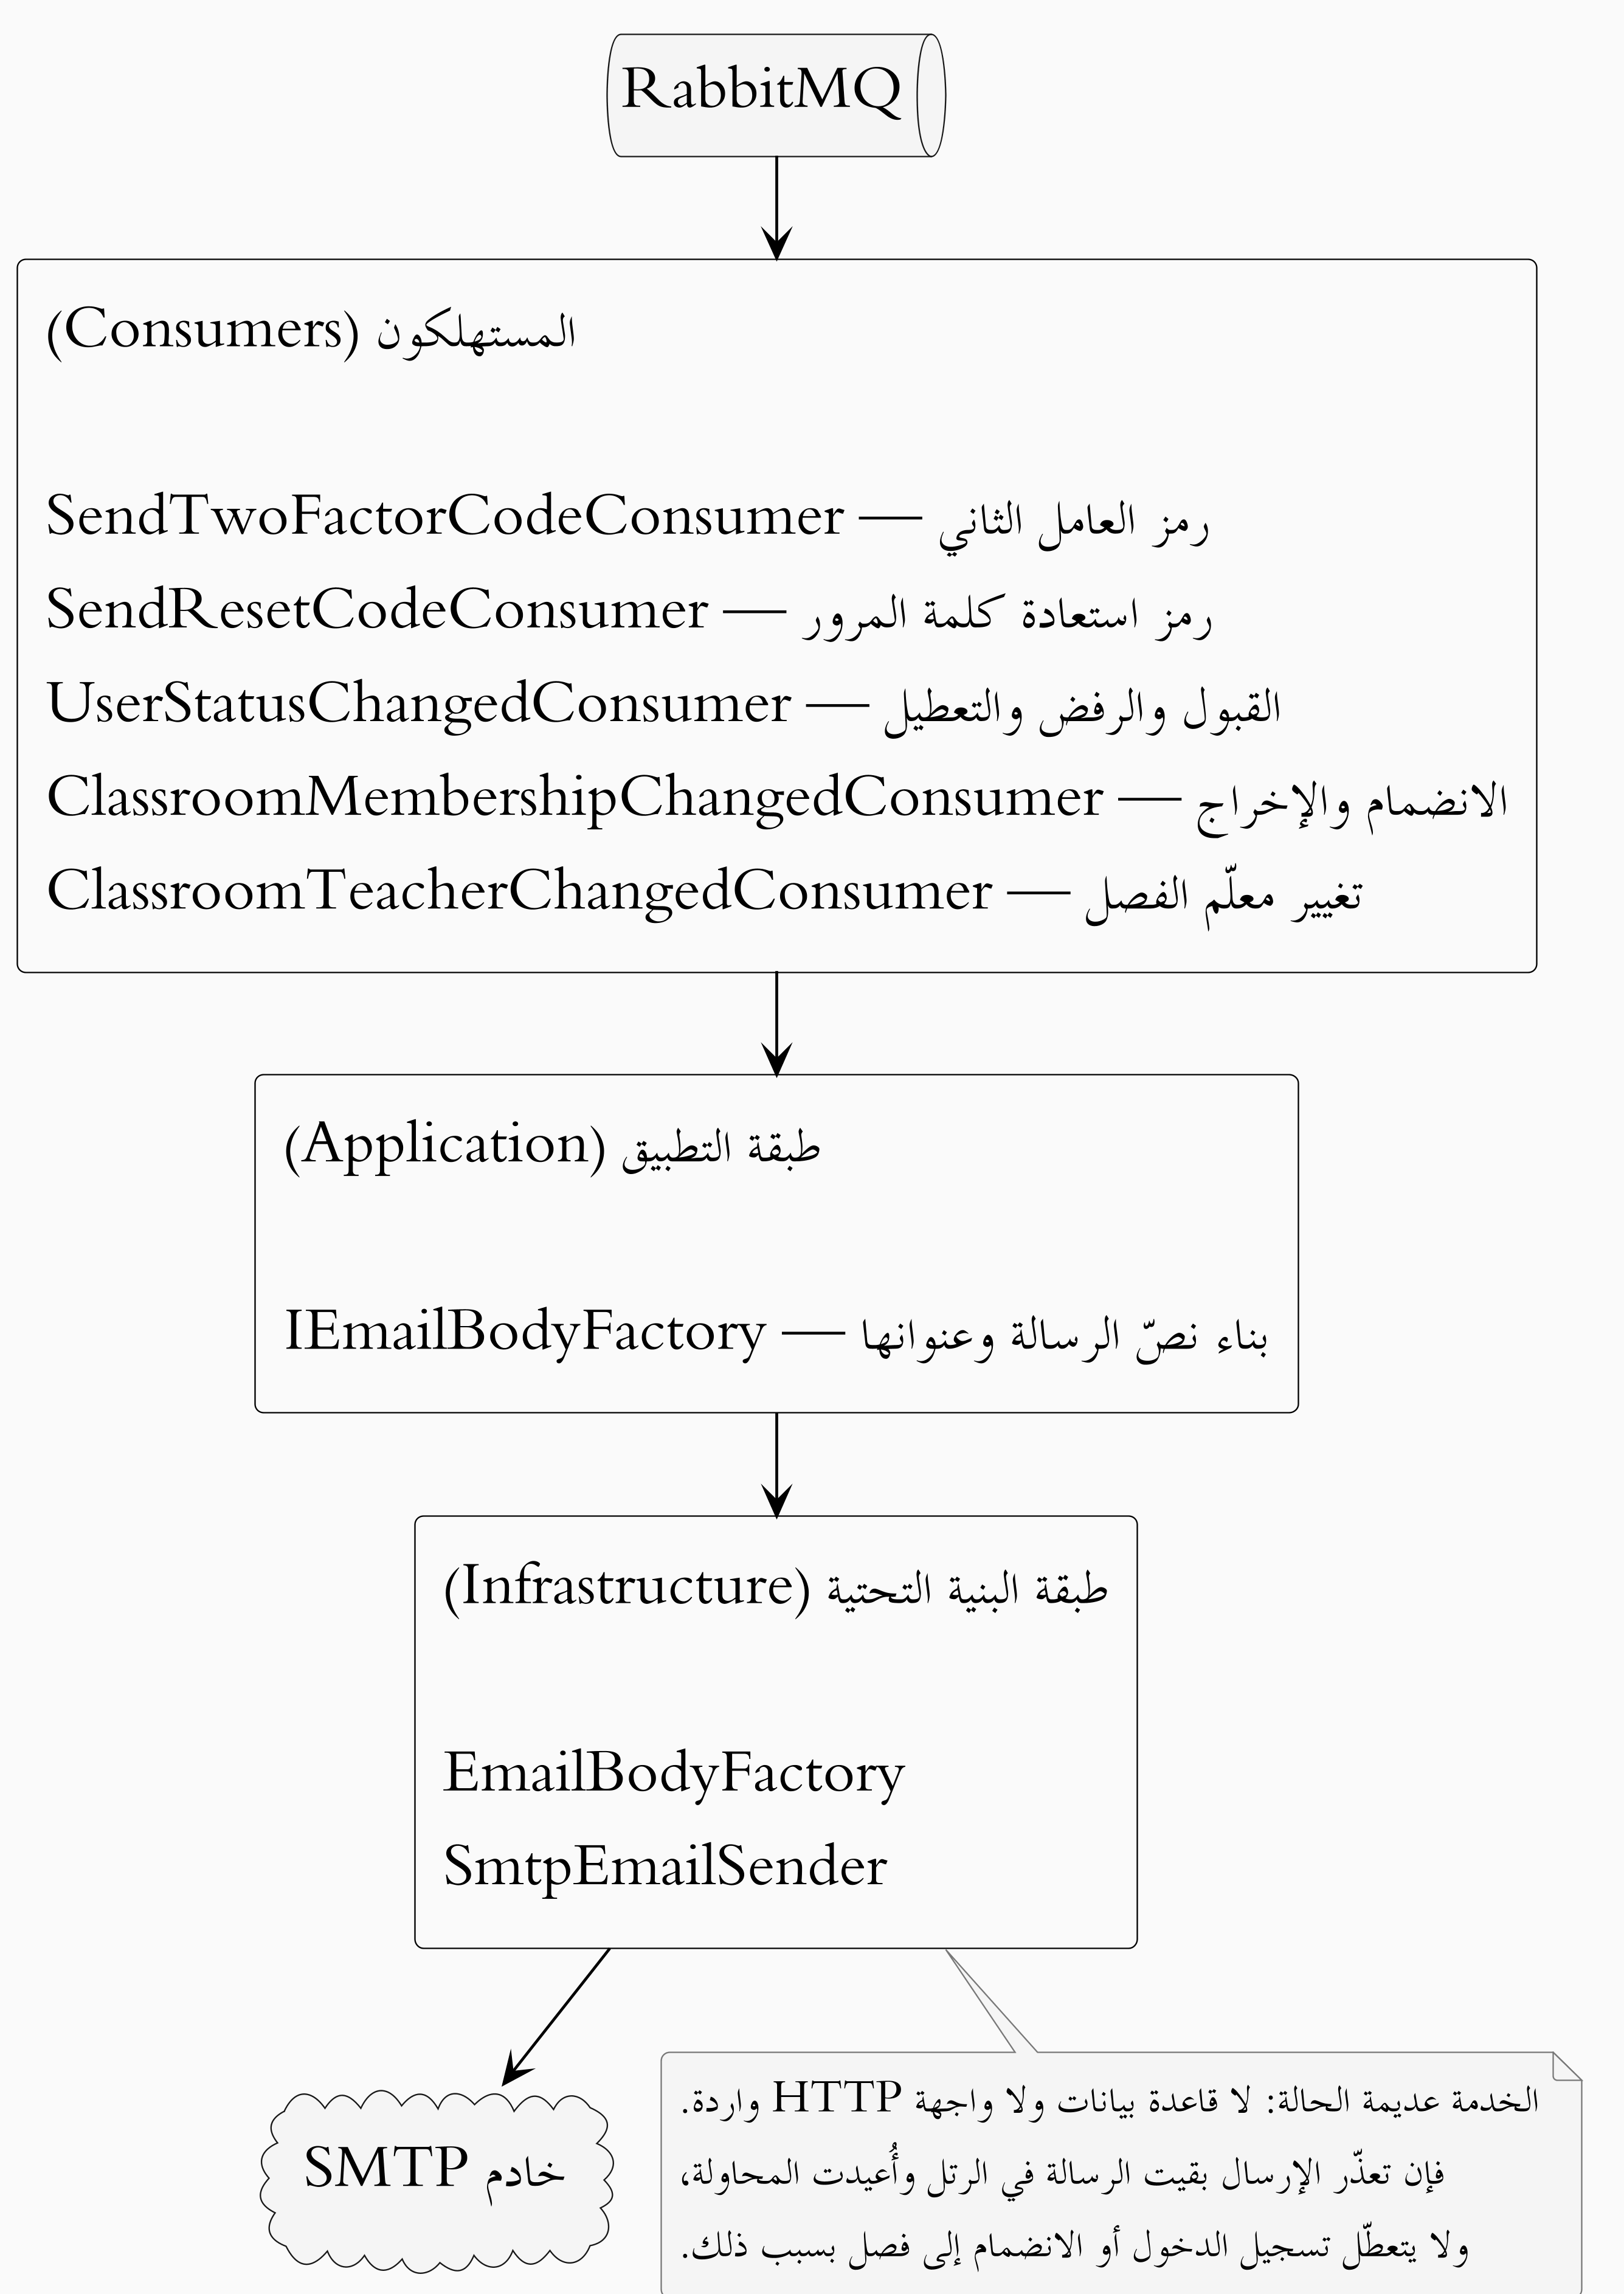
\includegraphics[width=\textwidth,height=0.8\textheight,keepaspectratio]{figures/comp-04-email.png}
  \caption{مخطط المكوّنات التفصيلي لخدمة البريد.}
  \label{fig:comp-04}
\end{figure}

ويُبيَّن مسار الإشعار من لحظة نشره إلى لحظة تسليمه، وما يحقّقه من فكِّ الارتباط الزمني، في القسم~\ref{subsubsec:flow-email}.


\section{خدمة الاسترجاع (\en{RagService})}
% Content for Chapter 5, Section 5.8 — pulled in by chapters/05-system-design.tex
\subsection{دور الخدمة ونطاقها}

% CH2-REF: originally ended "الموصوفة نظريًّا في القسم~\ref{sec:knowledge-pipeline}." — restore with chapter 2.
تحوّل خدمة المعرفة المواد المرجعية التي يرفعها المعلّم، من ملفّات \en{PDF} ومستندات \en{Word} وعروض \en{PowerPoint}، إلى قاعدة معرفية قابلة للبحث الدلالي تغذّي قدرات التوليد المعزّز بالاسترجاع (\en{RAG}). وتنفّذ الخدمة مرحلتين: الفهرسة (\en{Indexing}) والاسترجاع (\en{Retrieval})، فيُبنى فهرس دلالي لكل فصل دراسي تُؤصَّل به إجابات النظام في مادة ذلك الفصل.

\subsection{مكوّنات الخدمة}

يعرض الشكل~\ref{fig:comp-05} مكوّنات الخدمة وروابطها الخارجية، وهي مجمّعة بحسب المهامّ الأربع التي تؤدّيها: الاستيعاب والاسترجاع والتلخيص وإعادة التضمين.

\begin{figure}[htbp]
  \centering
  % Width to be re-checked when the draw.io export replaces this PNG.
  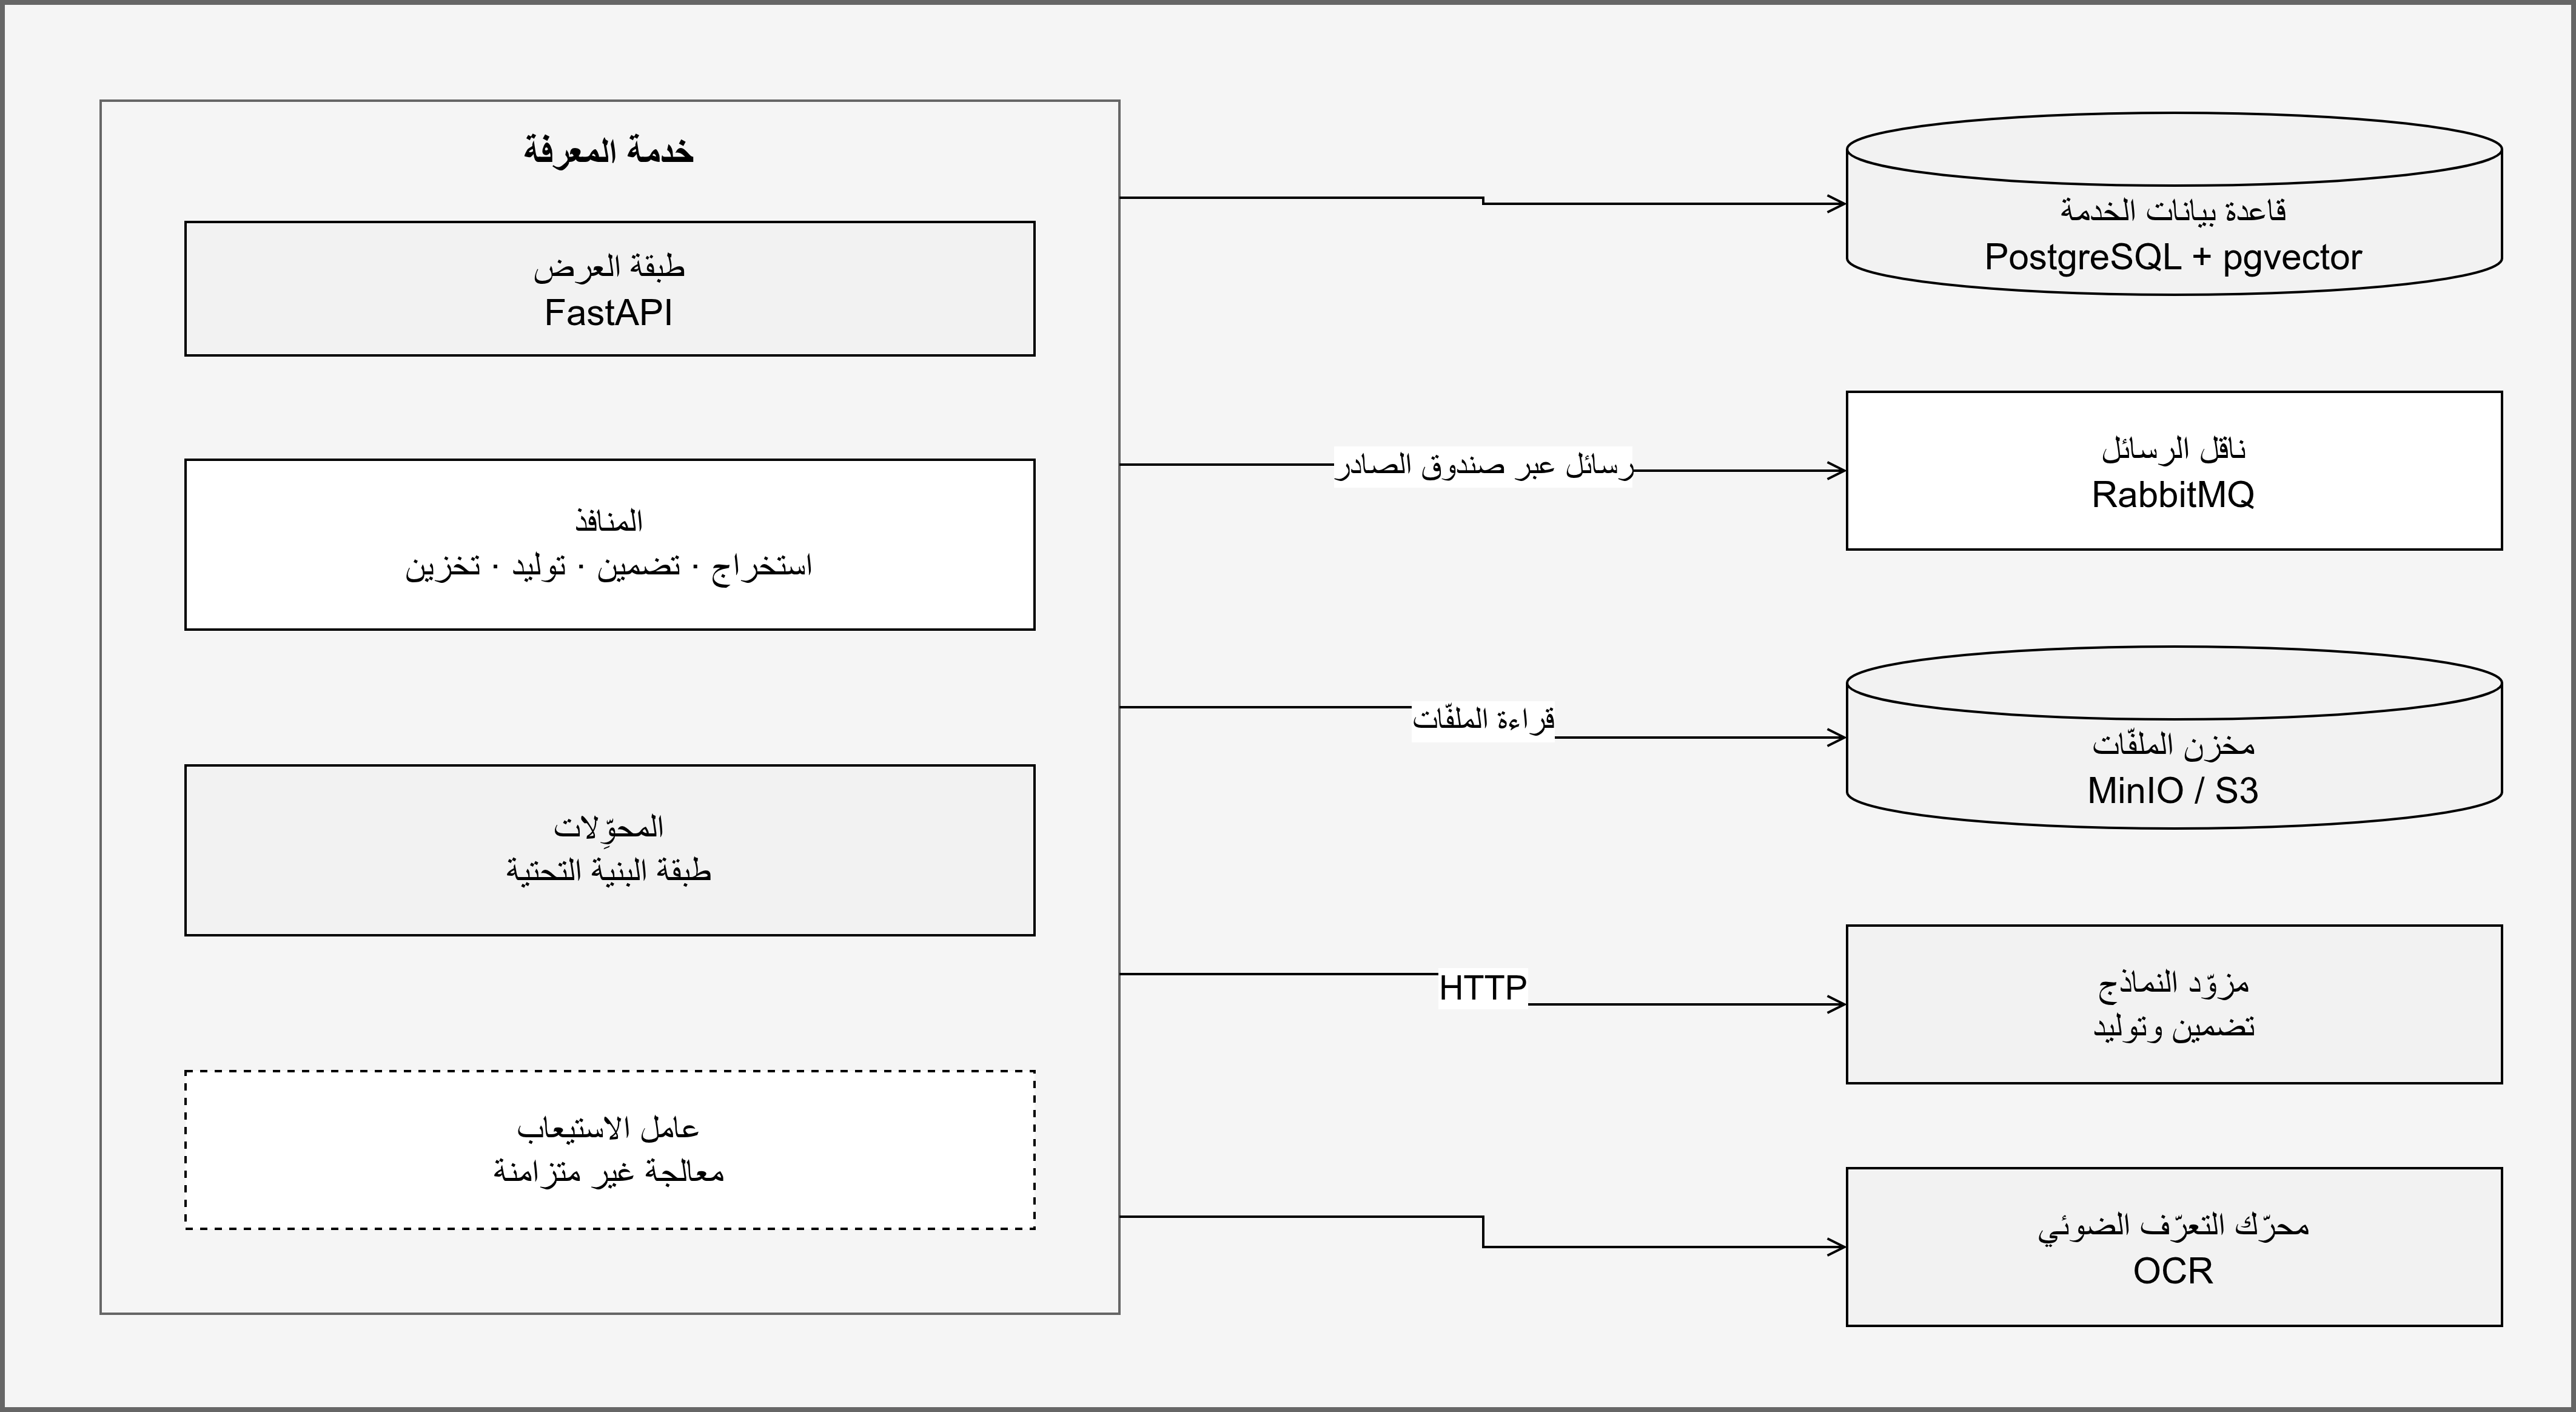
\includegraphics[width=\textwidth,height=0.8\textheight,keepaspectratio]{figures/comp-05-rag.png}
  \caption{مخطط مكوّنات خدمة المعرفة.}
  \label{fig:comp-05}
\end{figure}

وطُبّق في هذه الخدمة نمط المنافذ والمحوِّلات: تُعرّف طبقة التطبيق منافذ مجرّدة تصف ما تحتاجه الخدمة من استخراج وتضمين وتخزين، ويقع كل اختيار تقني خلف أحدها في طبقة البنية التحتية. ويحصر ذلك استبدال مزوّد التضمين أو محرّك التعرّف الضوئي في محوِّل واحد، دون تعديل منطق خط الأنابيب. ويعرض الشكل~\ref{fig:class-01} هذا التصميم مطبَّقاً على خط أنابيب الاستيعاب.

\begin{figure}[htbp]
  \centering
  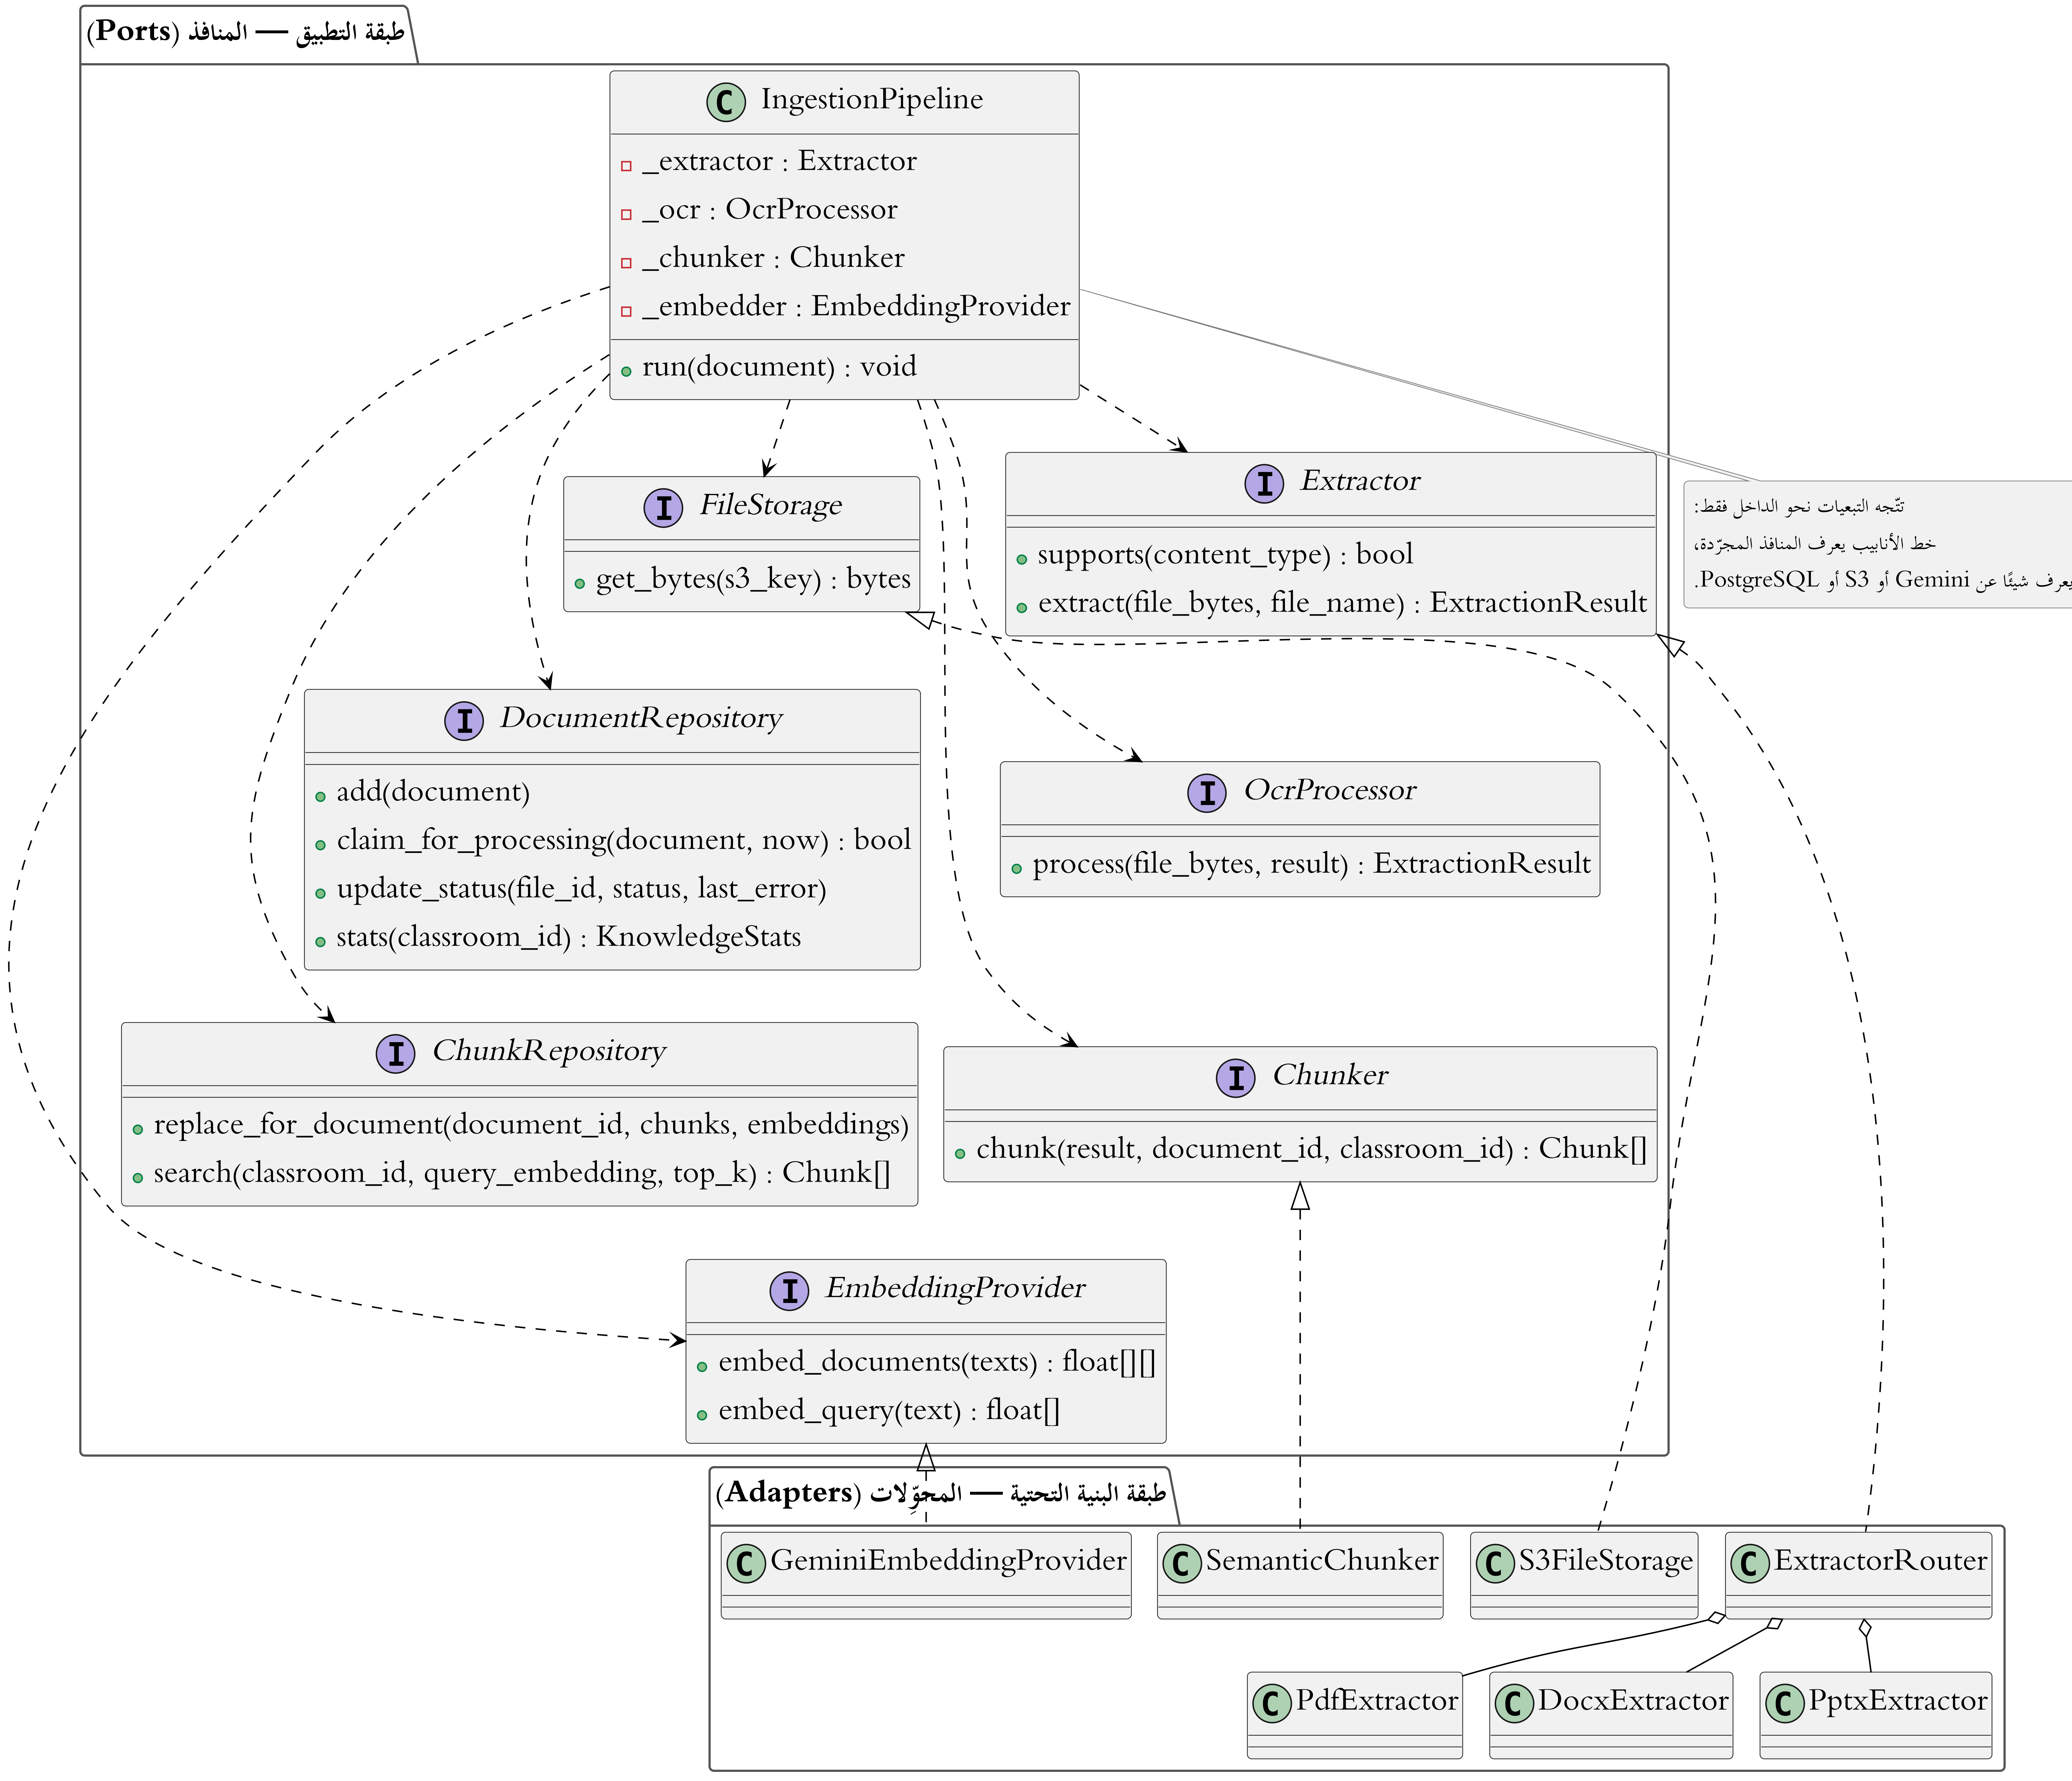
\includegraphics[width=\textwidth,height=0.8\textheight,keepaspectratio]{figures/class-01-ports-adapters.png}
  \caption{مخطط الصفوف لنمط المنافذ والمحوِّلات في خط أنابيب الاستيعاب.}
  \label{fig:class-01}
\end{figure}

\subsection{نموذج البيانات}
\label{subsec:rag-data-model}

يقوم نموذج البيانات على أربعة كيانات يعرضها الشكل~\ref{fig:erd-04}: المستند والمقطع، وسجلّات محاولات التلخيص، وجدول صندوق الصادر.

\begin{figure}[htbp]
  \centering
  % Width to be re-checked when the draw.io export replaces this PNG.
  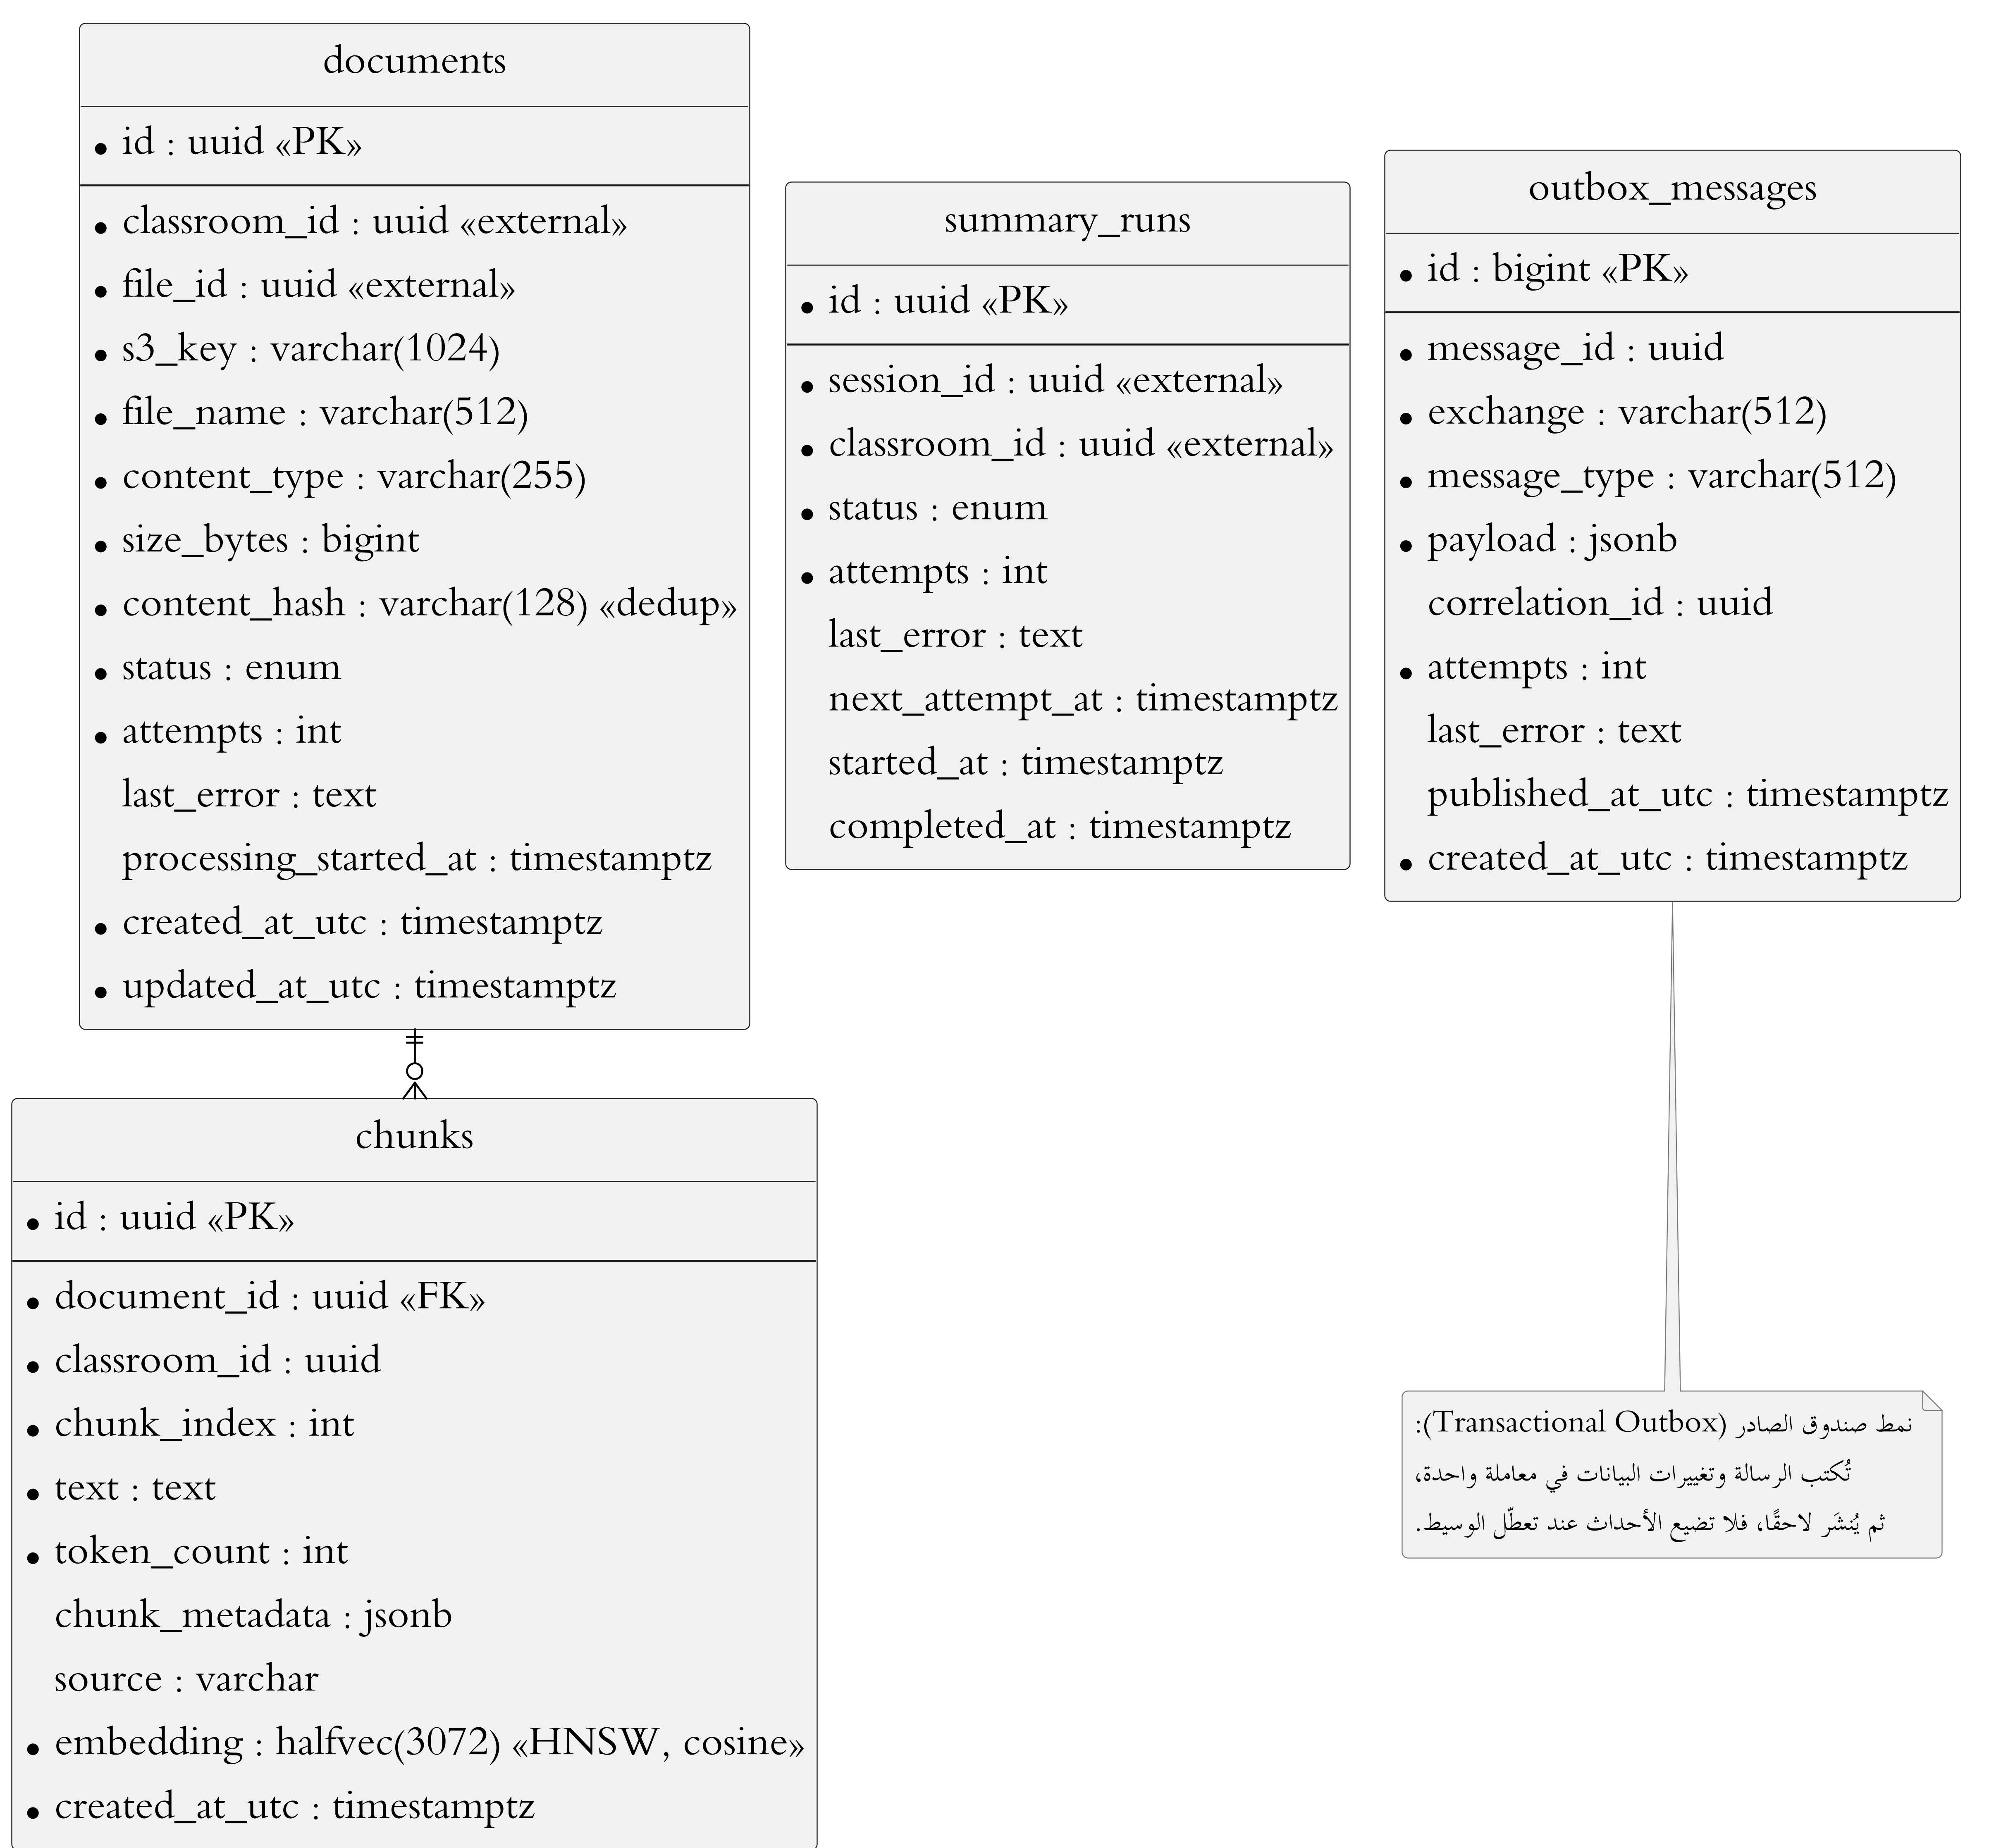
\includegraphics[width=\textwidth,height=0.8\textheight,keepaspectratio]{figures/erd-04-rag.png}
  \caption{مخطط الكيانات والعلاقات لخدمة المعرفة.}
  \label{fig:erd-04}
\end{figure}

ويتضمّن هذا النموذج قرارين تصميميين:

\begin{enumerate}
  \item \textbf{تضمين معرّف الفصل في كيان المقطع}: يتيح قصر البحث الدلالي على فصل بعينه، فيُعزَل محتوى كل فصل ولا يتسرّب إلى نتائج فصل آخر.
  \item \textbf{استعمال النوع \en{halfvec} لتخزين الأشعّة}: يبلغ طول شعاع التضمين 3072، وهو يتجاوز الحدّ الأقصى البالغ 2000 الذي يقبله فهرس \en{HNSW} للنوع \en{vector}. ويقبل النوع \en{halfvec} هذا الطول ويسمح بفهرسته.
\end{enumerate}


\section{خدمة المساعد المباشر (\en{LiveAssistantService})}
% Content for Chapter 5, Section 5.9 — pulled in by chapters/05-system-design.tex
\subsection{دور الخدمة ونطاقها}

تتابع هذه الخدمة الشرح أثناء الجلسة الحيّة، فتحوّل صوت المعلّم إلى نصّ، وتقارن ما يشرحه بالمادة المرجعية المفهرسة، وترسل إليه ملاحظة خاصّة عند رصد فرق أو نقص. وهي الخدمة الوحيدة التي يقوم مسارها الرئيس على حلقة مستمرّة تعمل طوال الجلسة، لا على دورة طلب وجواب.

\subsection{مكوّنات الخدمة}

تنتظم مكوّنات طبقة التطبيق مراحلَ متتابعة تمثّل هذه الحلقة: التقاط الصوت، وتحويله إلى نصّ، وكشف حدّ الفكرة، وتقييمها مقابل المصادر، وضبط إيقاع التدخّل، ثمّ إرساله. ويعرض الشكل~\ref{fig:comp-06} هذه المكوّنات وروابطها الخارجية.

% [H]: pinned under the paragraph that introduces it. At 2.09:1 full width is
% only ~32% of the text block, so it fits without shrinking.
\begin{figure}[H]
  \centering
  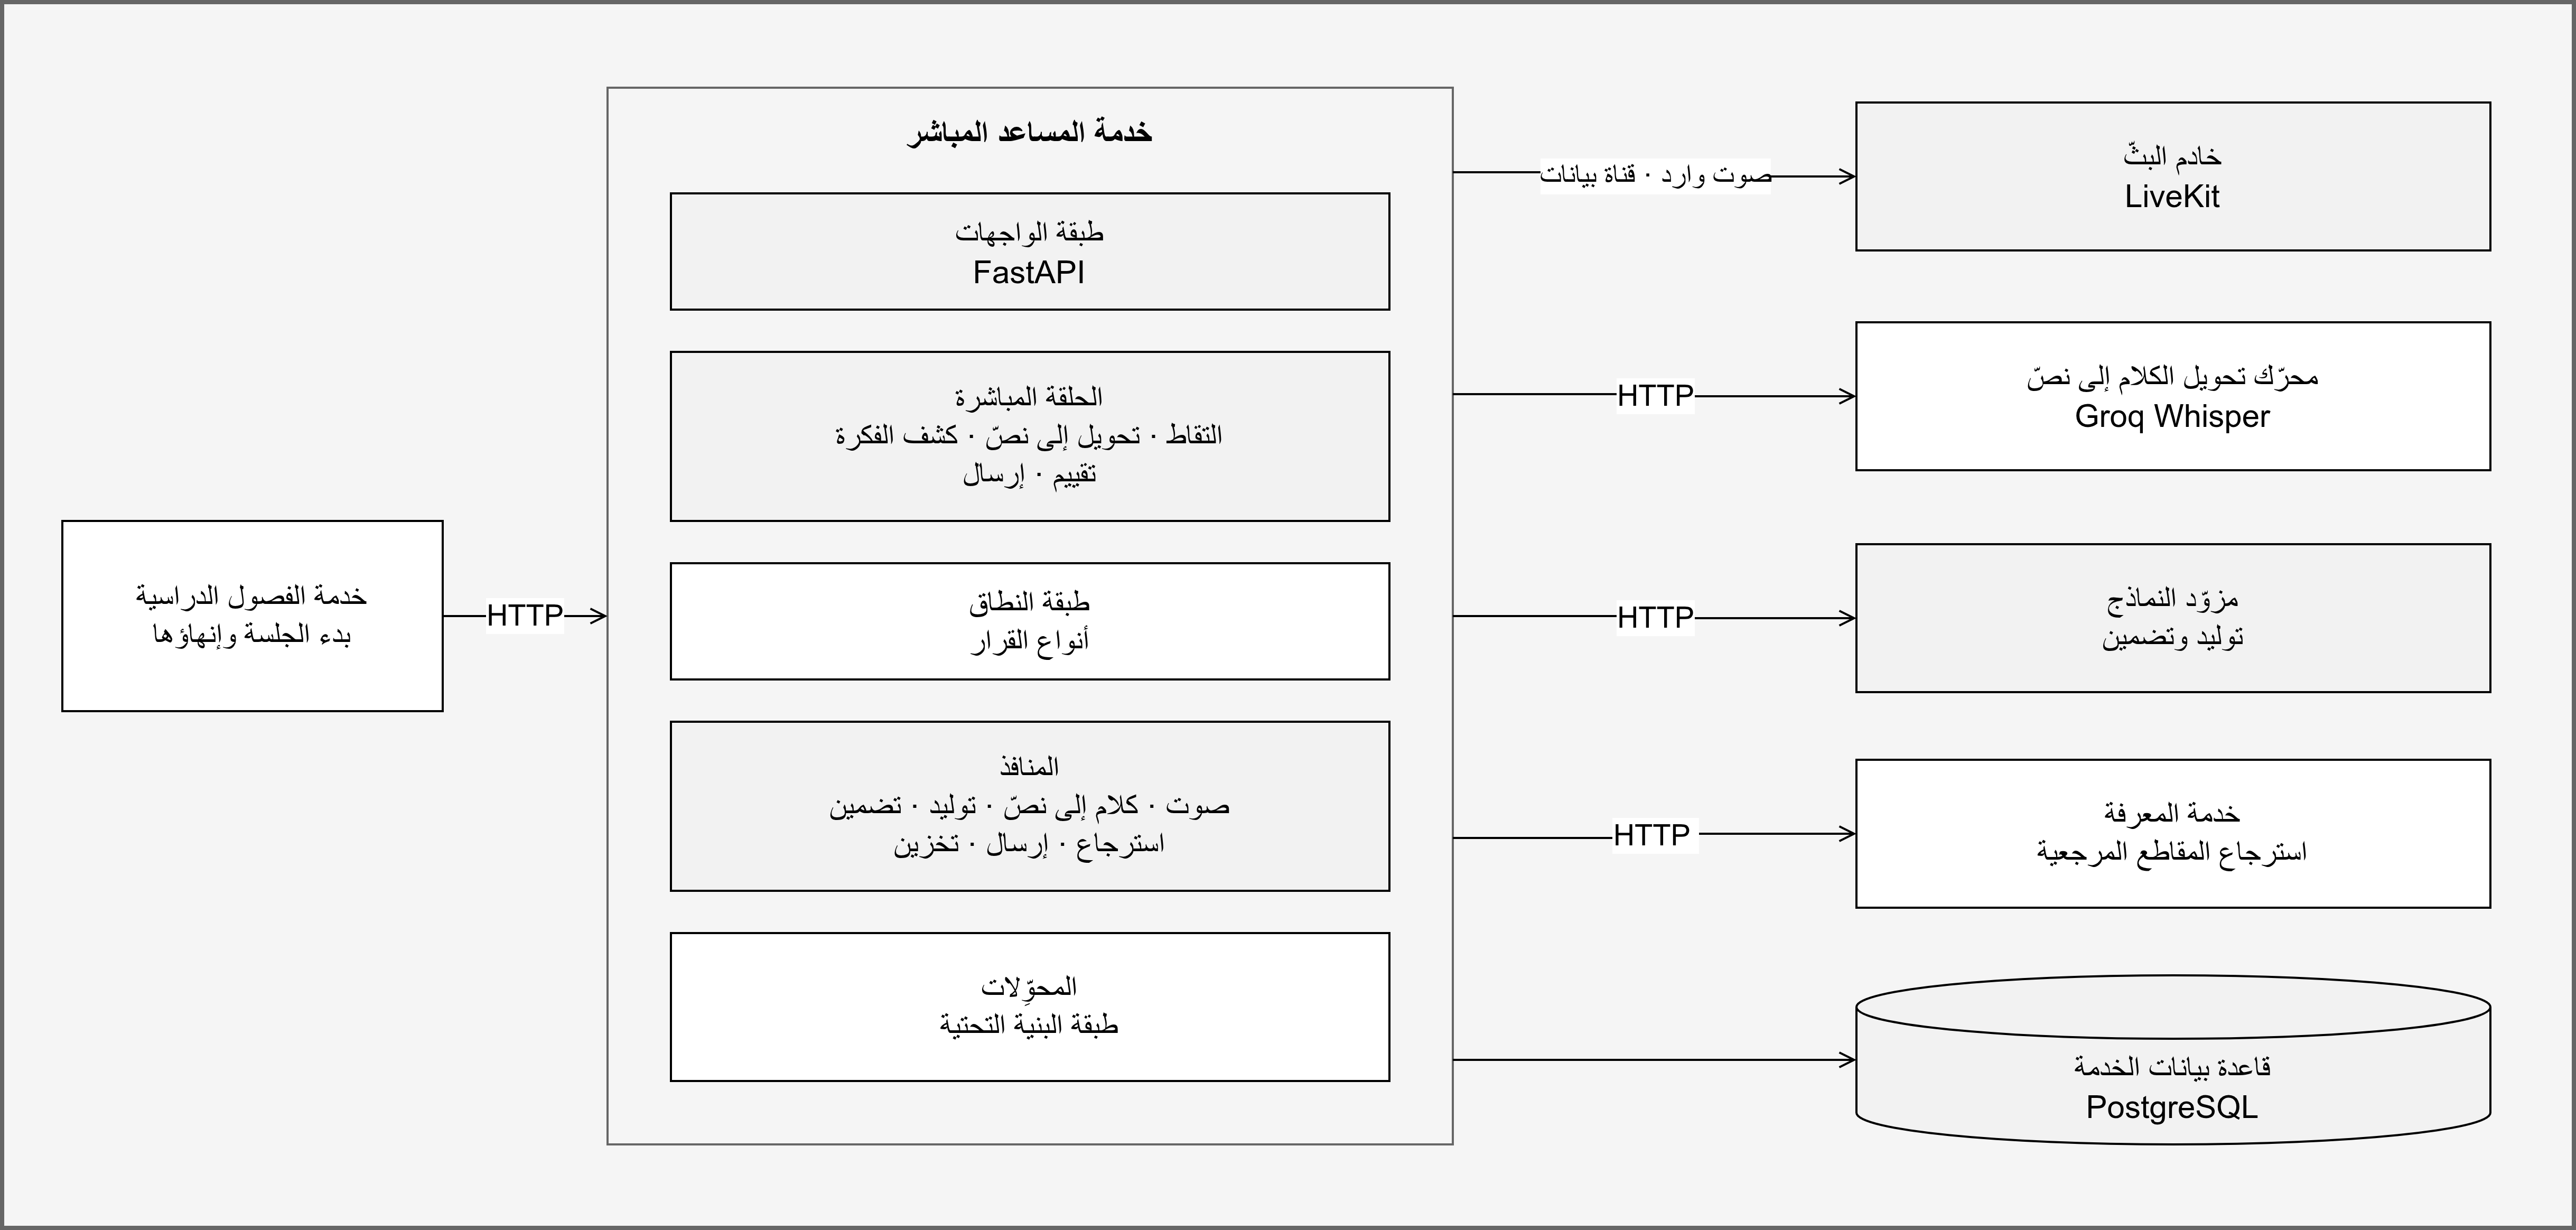
\includegraphics[width=\textwidth,height=0.8\textheight,keepaspectratio]{figures/comp-06-live-assistant.png}
  \caption{مخطط مكوّنات خدمة المساعد المباشر.}
  \label{fig:comp-06}
\end{figure}

وطُبّق في هذه الخدمة نمط المنافذ والمحوِّلات: يقابل كلَّ مورد خارجي منفذٌ مجرّد في طبقة التطبيق ومحوِّل واحد خلفه في طبقة البنية التحتية، وذلك لمصدر الصوت ومحرّك تحويل الكلام إلى نصّ والنموذج التوليدي ومزوّد التضمين وعميل الاسترجاع وقناة إرسال التدخّل ومستودع النصّ. ويتيح ذلك استبدال أيّ مزوّد دون تعديل منطق الحلقة، وتشغيل الحلقة كاملةً في الاختبارات بمحوِّلات بديلة لا تتّصل بشبكة.

وتحمل طبقة النطاق أنواع القرار نفسها: اكتمال الفكرة، ونتيجة التقييم ودرجة خطورتها، وقرار الإيقاع وسبب الكبح. وهي منطق خالص لا يستدعي نموذجًا ولا اتصالًا شبكيًّا ولا قاعدة بيانات، فتقبل الاختبار الوحدوي دون أيّ اعتماد خارجي.

ويفصل مُوقِّع التدخّل (\en{FeedbackPacer}) بين صحّة الملاحظة ووصولها إلى المعلّم، فيطبّق أربع قواعد بالترتيب، وتوقف أُولاها تحقّقًا الإرسالَ: حدّ أدنى لدرجة الثقة، وسقف لعدد التدخّلات في الجلسة الواحدة، وحدّ أدنى زمني بين تدخّلين متتاليين، ورفض الملاحظة المشابهة لما أُرسل ضمن نافذة زمنية محدّدة. والغرض منع مقاطعة المعلّم في أثناء الشرح.

وتُعرض الحلقة كاملةً، من التقاط الصوت إلى قرار التدخّل، في القسم~\ref{subsubsec:flow-live-loop}.

\subsection{نموذج البيانات}

لا تحفظ هذه الخدمة إلّا نصّ الجلسة؛ أمّا التسجيل والملخّص فيقعان في خدمة الفصول الدراسية ومخزن الملفّات. ويقوم النموذج على كيانين يعرضهما الشكل~\ref{fig:erd-05}: ترويسة النصّ (\en{session\_transcripts}) ومقاطعه المرتّبة زمنيًّا (\en{transcript\_segments}).

% [H]: pinned under the paragraph that introduces it. At 2.63:1 full width is
% only ~26% of the text block, so it fits without shrinking.
\begin{figure}[H]
  \centering
  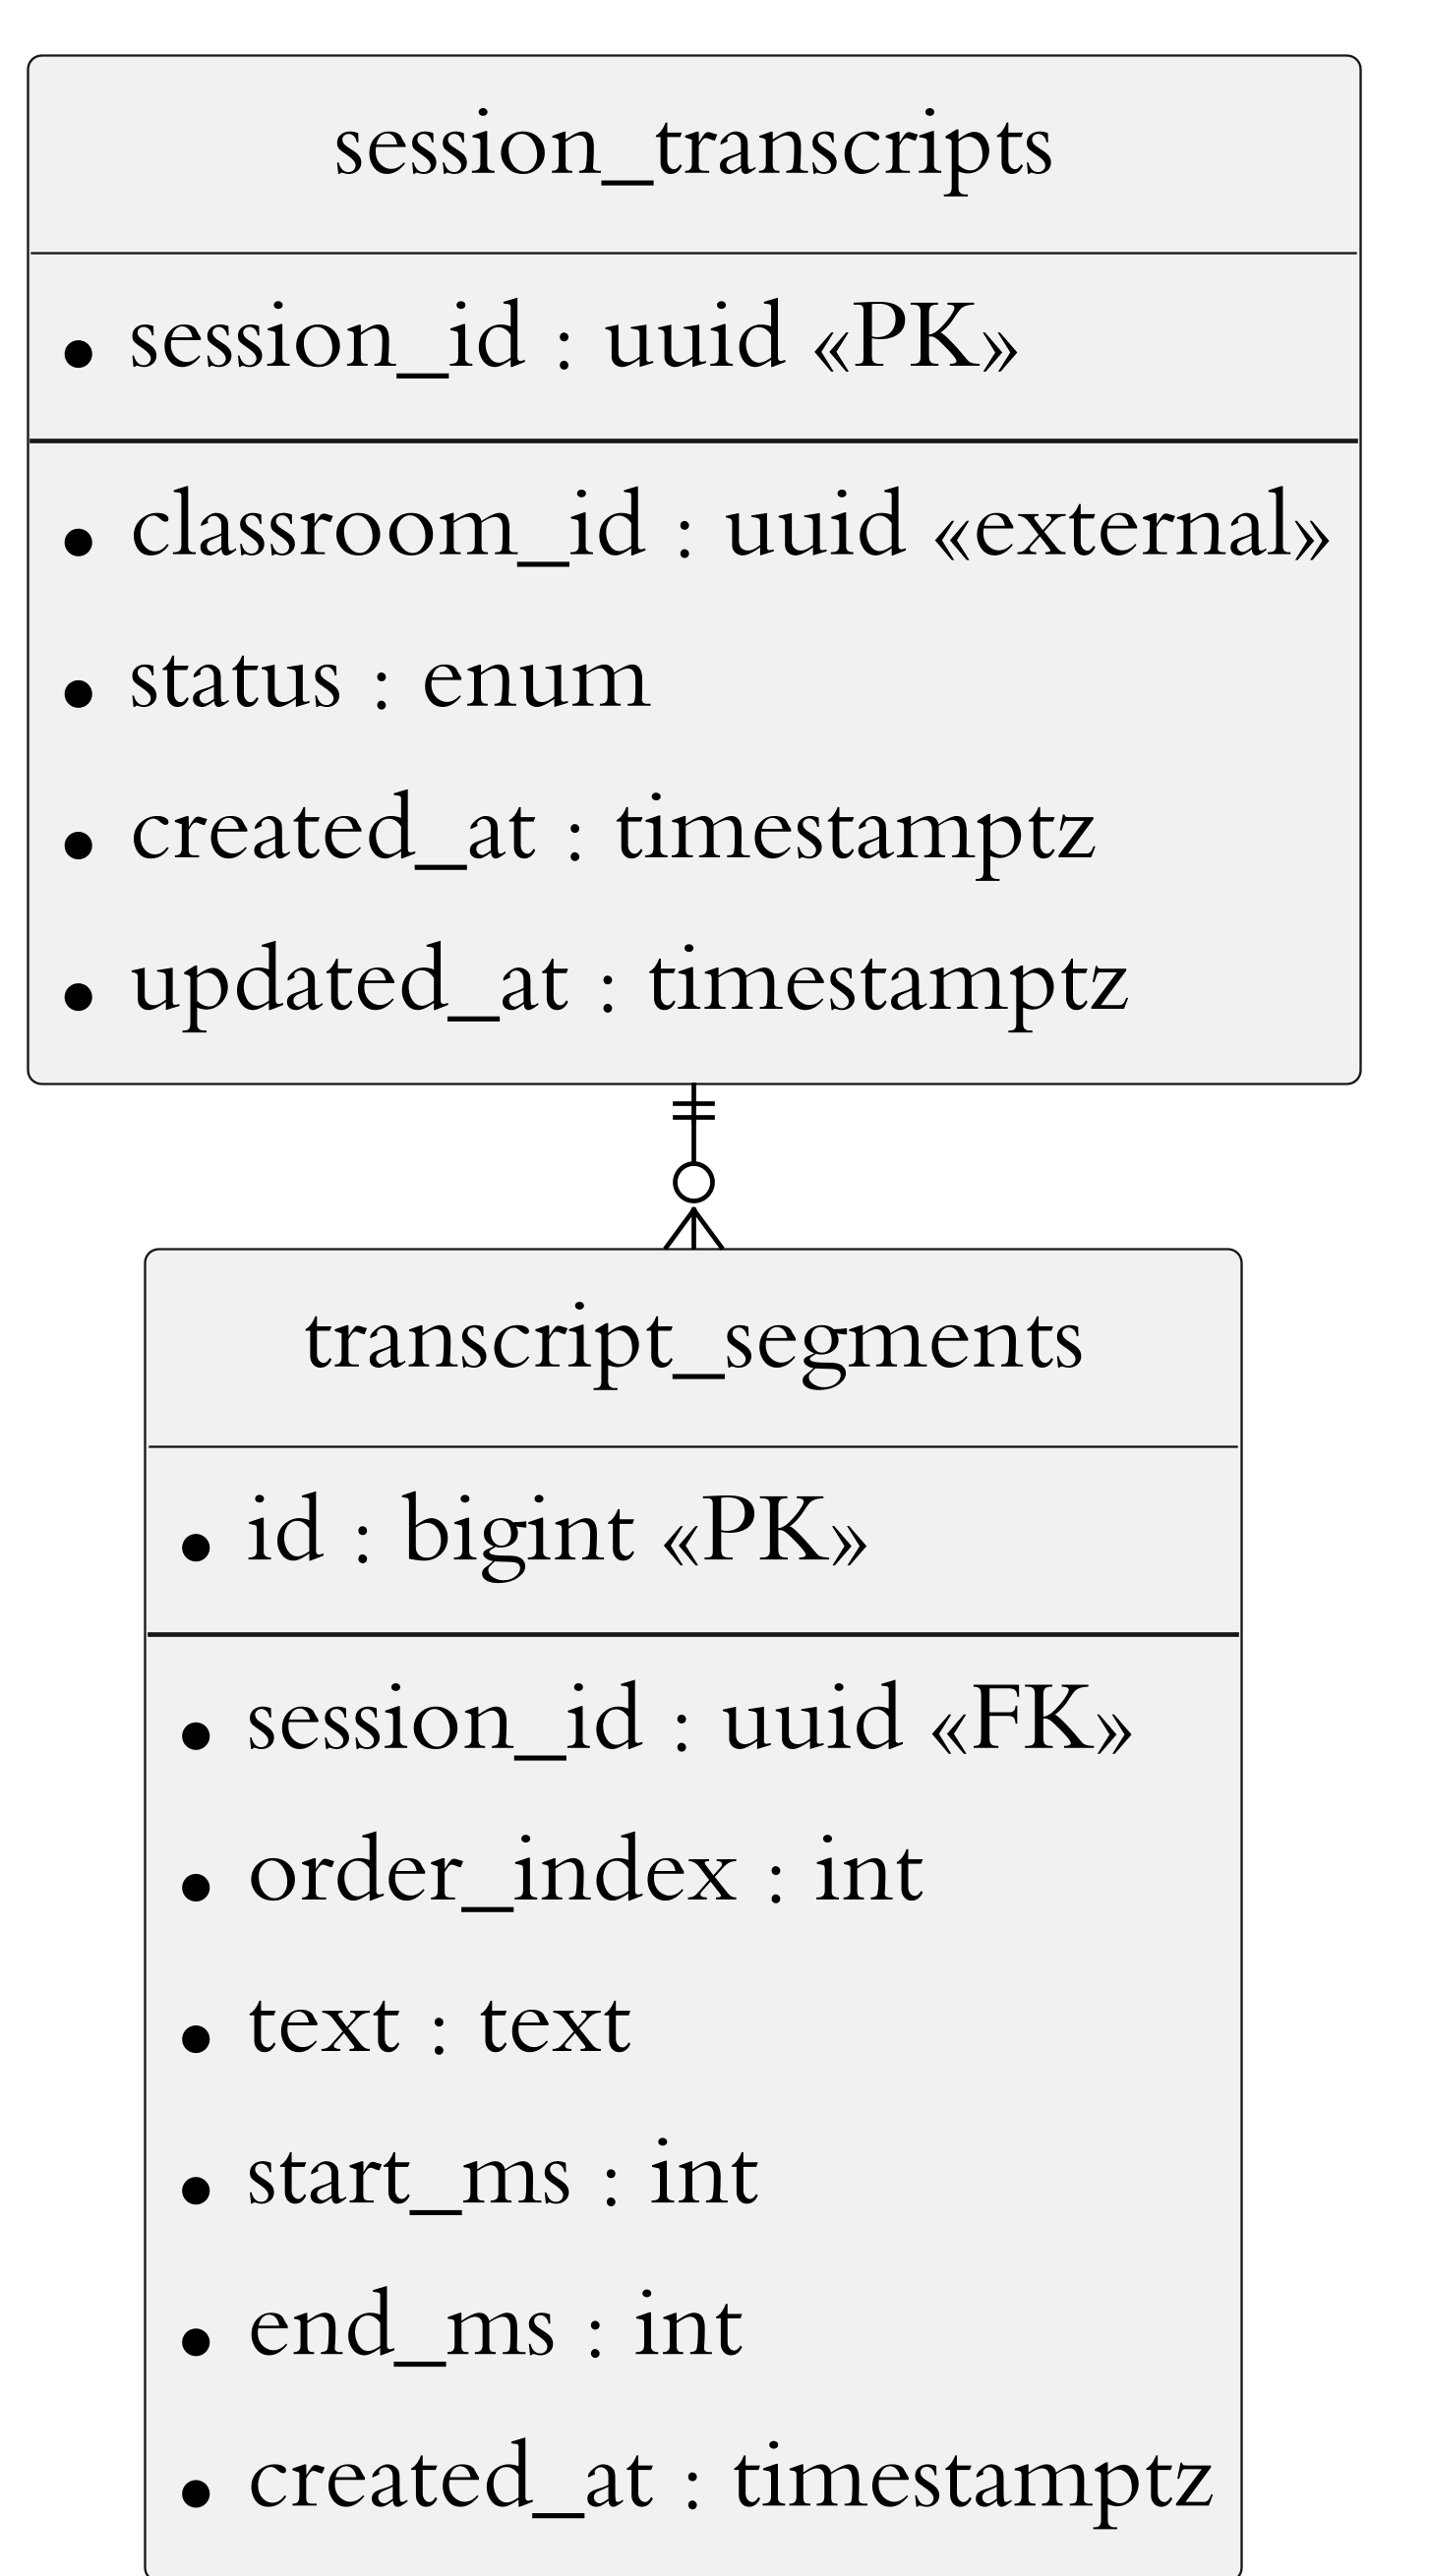
\includegraphics[width=\textwidth,height=0.8\textheight,keepaspectratio]{figures/erd-05-live-assistant.png}
  \caption{مخطط الكيانات والعلاقات لخدمة المساعد المباشر.}
  \label{fig:erd-05}
\end{figure}

ويضبط قيدُ فرادة مركّب على الزوج (\en{session\_id}, \en{order\_index}) تسلسلَ المقاطع داخل الجلسة ويمنع تكرار الرقم نفسه، في حين يؤدّي حذف الترويسة إلى حذف مقاطعها تتابعيًّا.

